% -*- Mode:TeX -*-

%% IMPORTANT: The official thesis specifications are available at:
%%            http://libraries.mit.edu/archives/thesis-specs/
%%
%%            Please verify your thesis' formatting and copyright
%%            assignment before submission.  If you notice any
%%            discrepancies between these templates and the 
%%            MIT Libraries' specs, please let us know
%%            by e-mailing thesis@mit.edu

%% The documentclass options along with the pagestyle can be used to generate
%% a technical report, a draft copy, or a regular thesis.  You may need to
%% re-specify the pagestyle after you \include  cover.tex.  For more
%% information, see the first few lines of mitthesis.cls. 

%\documentclass[12pt,vi,twoside]{mitthesis}
%%
%%  If you want your thesis copyright to you instead of MIT, use the
%%  ``vi'' option, as above.
%%
%\documentclass[12pt,twoside,leftblank]{mitthesis}
%%
%% If you want blank pages before new chapters to be labelled ``This
%% Page Intentionally Left Blank'', use the ``leftblank'' option, as
%% above. 

\documentclass[12pt,twoside]{mitthesis}
\usepackage{lgrind}
%% These have been added at the request of the MIT Libraries, because
%% some PDF conversions mess up the ligatures.  -LB, 1/22/2014
\usepackage{cmap}
\usepackage[T1]{fontenc}
\usepackage{tikz}
\usepackage[subpreambles=true]{standalone}
\usepackage[shortlabels]{enumitem}
\usetikzlibrary{shapes, arrows, decorations.markings}
\usepackage{amsmath,bm,times}
\usepackage{verbatim}
\usepackage{amsfonts}
\usepackage{etex}
\usetikzlibrary{calc,through,intersections}
\usepackage[many]{tcolorbox}
\usepackage{array}
\usepackage{amsthm}
\usepackage{booktabs}
\usepackage{cite}
\usepackage{url}
\usetikzlibrary{shadows.blur,shadings}
\pgfdeclarelayer{bg}    % declare background layer
\pgfsetlayers{main,bg}  % set the order of the layers (main is the standard layer)
%-------------------------------------------------MACROS--------------------------------------------------------------------------------
%%--------------------------------------------DEMOS-------------------------------------

\newcommand{\mb}{\mathbb}
\newcommand{\tb}[1]{\tilde{\mathbb{#1}}}
\newcommand{\mr}{\mathrm}
\newcommand{\mc}{\mathcal}
\newcommand{\tc}[1]{\tilde{\mathcal{#1}}}
\newcommand{\mbf}{\mathbf}
\newcommand{\msf}{\mathsf}
\newcommand{\Ch}{\mathsf{Ch}}
\newcommand{\mcP}{\mathcal{P}}
\newcommand{\A}{\mathcal{A}}
\newcommand{\Pol}{\mathcal{P}}
\newcommand{\negl}{\mathsf{negl}}
\newcommand{\poly}{\mathsf{poly}}
\newcommand{\la}{\lambda}
\newcommand{\bin}[2]{#1_{n-1}\cdots#1_{#2}}
\newcommand{\Si}{\mathcal{S}}

\newcommand{\set}[1]  {\left\{#1\right\}}
\newcommand{\abs}[1]  {\left|#1\right|}
\newcommand{\odds}[1] {\mathsf{odds}\left(#1\right)}
\newcommand{\floor}[1]{\lfloor #1\rfloor}
\newcommand{\ceil} [1]{\lceil #1\rceil}

\newcommand{\pick} [1] {\overset{#1}{\leftarrow}}
\newcommand{\Adv}{\mathsf{Adv}}
\newcommand{\bind}{\mathsf{bind}}
\newcommand{\hide}{\mathsf{hide}}


\newcommand{\param}{\mathsf{Param}}
\newcommand{\DL}{\mathsf{Dlog}}
\newcommand{\pk}{\mathsf{pk}}
\newcommand{\sk}{\mathsf{sk}}
\newcommand{\Gen}{\mathsf{Gen}}
\newcommand{\Enc}{\mathsf{Enc}}
\newcommand{\Dec}{\mathsf{Dec}}
\newcommand{\accept}{\mathsf{accept}}
\newcommand{\reject}{\mathsf{reject}}
\newcommand{\Sig}{\mathsf{Sig}}
\newcommand{\GenBP}{\mathsf{Gen}_{\mathsf{bp}}}
\newcommand{\Opt}{\mathsf{Opt}}

\newcommand{\VerSig}{\mathsf{Ver}_{\mathsf{sig}}}

%commitment
\newcommand{\Com}  {\mathsf{Com}}
\newcommand{\ck}{\mathsf{ck}}
\newcommand{\Ver}{\mathsf{Ver}}

\newcommand{\view}{\mathsf{view}}



\renewcommand{\vec}[1]{\mathbf{#1}}
\newcommand{\vect}[1]{\overset{\rightarrow}{#1}}

\newcommand{\eatitemspace}{}

\newcommand{\putbox}{\hspace*{\fill}$\Box$}



\newcommand{\Prob}{\mbox{\( \mathbf{ Prob } \)}}

\def\squareforqed{\hbox{\(\blacksquare\)}}
\def\qed{\ifmmode\squareforqed\else{\unskip\nobreak\hfill\penalty50\hskip1em\null\nobreak\hfil\squareforqed\parfillskip=0pt\finalhyphendemerits=0\endgraf}\fi}
\setlength\belowrulesep{0pt}
\setlength\aboverulesep{-1.3pt}
\newcommand{\thickhline}{\midrule[1.2pt]}
\newcommand{\bad}{\mathsf{bad}}


\DeclareMathAlphabet\mathbfcal{OMS}{cmsy}{b}{n}
\newcommand{\VS}{\mathbfcal{VS}}
\newcommand{\VCr}{\mathbfcal{VC}}
\newcommand{\EA}{\mathsf{EA}}
\newcommand{\BB}{\mathsf{BB}}
\newcommand{\BDS}{\mathsf{BDS}}
\newcommand{\VSD}{\mathsf{VSD}}
\newcommand{\ASD}{\mathsf{ASD}}
\newcommand{\VC}{\mathsf{VC}}
\newcommand{\CD}{\mathsf{CD}}
\newcommand{\Admin}{\mathsf{Admin}}
\newcommand{\info}{\mathsf{info}}
\newcommand{\aux}{\mathsf{aux}}
\newcommand{\st}{\mathsf{st}}
\newcommand{\vid}{\mathsf{vid}}
\newcommand{\ch}{\mathsf{Ch}}

\newcommand{\cala}{\mathcal{A}}
\newcommand{\calb}{\mathcal{B}}
\newcommand{\calc}{\mathcal{C}}
\newcommand{\cals}{\mathcal{S}}
\newcommand{\calr}{\mathcal{R}}
\newcommand{\calm}{\mathcal{M}}
\newcommand{\calk}{\mathcal{K}}
\newcommand{\calx}{\mathcal{X}}
\newcommand{\caly}{\mathcal{Y}}
\newcommand{\calf}{\mathcal{F}}
\newcommand{\Z}{\mathcal{Z}}
\newcommand{\calp}{\mathcal{P}}
\newcommand{\calv}{\mathcal{V}}
\newcommand{\call}{\mathcal{L}}
\newcommand{\calo}{\mathcal{O}}
\newcommand{\calu}{\mathcal{U}}
\newcommand{\calt}{\mathcal{T}}

\newcommand{\ZZ}{\mathbb{Z}}
\newcommand{\GF}{\mathbb{GF}}
\newcommand{\GG}{\mathbb{G}}

\newcommand{\Open}{\mathsf{Open}}
\newcommand{\SXDH}{\mathsf{sxdh}}
\newcommand{\Sim}{\mathsf{Sim}}
\newcommand{\td}{\mathsf{td}}
\newcommand{\Prov}{\mathsf{Prov}}
\newcommand{\Vrfy}{\mathsf{Vrfy}}
\newcommand{\crs}{\mathsf{crs}}
%\newcommand{\ch}{\mathsf{ch}}
\newcommand{\opt}{\mathsf{opt}}
\newcommand{\rec}{\mathsf{rec}}
\newcommand{\eid}{\mathsf{eid}}
%\newcommand{\hash}{\mathsf{hash}}



\newcommand{\NIZK}{\mathsf{NIZK}}

\newcommand{\name}{PoWorK}
\newcommand{\steps}{\msf{Steps}}


\newcommand{\Setup}{\mathbf{Setup}}
\newcommand{\Cast}{\mathbf{Cast}}
\newcommand{\Tally}{\mathbf{Tally}}
\newcommand{\Result}{\mathbf{Result}}
\newcommand{\Verify}{\mathbf{Verify}}

\newcommand{\blt}{\mathbf{blt}}
\newcommand{\ta}{\mathbf{ta}}

%%%%%%%%%%%%%%%%%%%%%%%%%%%%%%%%%%%%%%%%%%%%
%-------------------------ENVIRONMENTS---------------------------------------------------

\newenvironment{proofsketch}{\noindent\textit{Proof sketch:}}{\putbox}
\newenvironment{PhDproof}{\noindent {\em Proof:}}{\putbox}
%
\newenvironment{boxfig}[2]{%
     \begin{figure}[h!]
     \newcommand{\FigCaption}{#1}
     \newcommand{\FigLabel}{#2}
%     \vspace{-0.25cm}
     \begin{center}
       \begin{small}
         \begin{tabular}{@{}|@{~~}l@{~~}|@{}}
           \hline
           \rule[-1.5ex]{0pt}{1ex}\begin{minipage}[b]{.9\linewidth}
             \vspace{1ex}
             \smallskip
             }{%
           \end{minipage}\\
           \hline
         \end{tabular}
       \end{small}
%       \vspace{-0.25cm}
      \caption{\FigCaption}
%       \figlab{\FigLabel}
     \end{center}
     \vspace{-0.5cm}
   \end{figure}
}
%
%
\newtcolorbox{phdshadebox}[1][]{
  enhanced, %drop shadow east,
  boxrule=1.5pt,arc=.3em,boxsep=-1mm,
  left=.5em,right=.5em,top=5pt,bottom=5pt,
  colback=white,#1
}
%
\newenvironment{shadowfig}[2]{%
     \begin{figure}[H]
     \newcommand{\FigCaption}{#1}
     \newcommand{\FigLabel}{#2}
     \begin{phdshadebox}
%
\begin{center}
\begin{small}
\begin{minipage}{0.95\linewidth}
\medskip
%
}{
%
\smallskip
\end{minipage}
\end{small}
\end{center}
\end{phdshadebox}
\smallskip
  \caption{\FigCaption}
    \label{\FigLabel}
\end{figure}
}


\newenvironment{experiment}{
%\medskip
\begin{center}\begin{boxedminipage}{\linewidth}}{\end{boxedminipage}\end{center}
%\medskip
}

%
\newtcolorbox{shadebox}[1][]{
  enhanced,drop shadow shouthwest,
  boxrule=1pt,arc=1pt,boxsep=0pt,
  left=.5em,right=.5em,top=1ex,bottom=1ex,
  colback=white,#1
}
%
%
\newtcolorbox{eqbox}[1][]{
  enhanced, %drop shadow east,
  boxrule=1pt,arc=2mm, outer arc=2mm,boxsep=-1mm,colframe=mygray!20!black,
  left=.5em,right=.5em,top=10pt,bottom=10pt,halign=center,fuzzy shadow={2pt}{-2pt}{0pt}{0.2pt}{mygray},%drop large lifted shadow,
  colback=white, attach boxed title to top center={yshift=-0.8mm},#1
}
%
\newtcolorbox{stepbox}[1][]{
  enhanced,%drop shadow shouthwest,
  boxrule=0.75pt,arc=1pt,boxsep=0mm,
  left=.25em,right=.25em,top=10pt,bottom=10pt, attach boxed title to top center={yshift=-0.8mm},
  colback=white,#1
}

\tikzset{% 
    trustee/.style={%
        draw,align = center, text width = 32pt, text height = 20pt,line width=1.2pt,rounded corners=2pt,fill = white, 
        blur shadow={shadow xshift=2pt}
        }
}

\tikzset{% 
    voter/.style={%
        draw,circle,align = center, text width = 18pt, line width=1.2pt,fill = white, blur shadow={shadow xshift=1pt}
    }
}
\tikzset{% 
    human/.style={%
        draw,circle,align = center, text width = 16pt, line width=1.2pt,fill = white, drop shadow={shadow xshift=2.5pt, shadow yshift=-1.5pt, fill=mygray}
    }
}

\tikzset{% 
    SD/.style={%
        draw,align = center, text width = 27pt, text height = 15pt,line width=1.2pt,rounded corners=2pt,fill = white, 
       drop shadow={shadow xshift=2.5pt, shadow yshift=-1.5pt, fill=mygray}
        }
}
\tikzset{
sarrow/.style={
  draw,
  double arrow,
  text width=15pt,
  text height=10pt,
  fill=black
  }}
%%extractor
\newcommand{\Ext}{\mathsf{Ext}}
\newcommand{\pok}{\mathit{PoK}}
\newcommand{\pow}{\mathit{PoW}}

%%puzzle
\newcommand{\true}{\mathsf{true}}
\newcommand{\false}{\mathsf{false}}
\newcommand{\puz}{\mathsf{puz}}
\newcommand{\soln}{\mathsf{soln}}
\newcommand{\PuzSys}{\mathsf{PuzSys}}
\newcommand{\GenP}{\mathsf{GenPuz}}
\newcommand{\SolveP}{\mathsf{Solve}}
\newcommand{\Sample}{\mathsf{Sample}}
\newcommand{\SampleP}{\mathsf{SampleSol}}
\newcommand{\VerP}{\mathsf{Verify}}
\newcommand{\PuzzleS}{\mathcal{PS}}
\newcommand{\HardS}{\mathcal{HS}}
\newcommand{\SolutionS}{\mathcal{SS}}
\newcommand{\Params}{\mathsf{params}}
\newcommand{\LSB}{\mathsf{LSB}}
\newcommand{\CS}{\mathcal{CS}}

\newcommand{\AAA}{\mathcal{A}}
\newcommand{\BBB}{\mathcal{B}}
\newcommand{\EEE}{\mathsf{E}}
\newcommand{\FFF}{\mathcal{F}}
\newcommand{\CCC}{\mathcal{C}}
\newcommand{\DDD}{\mathcal{D}}
\newcommand{\III}{\mathcal{I}}
\newcommand{\RRR}{\mathcal{R}}
\newcommand{\LLL}{\mathcal{L}}
\newcommand{\KKK}{\mathcal{K}}
\newcommand{\PPP}{\mathsf{P}}
\newcommand{\VVV}{\mathsf{V}}
\newcommand{\SSS}{\mathcal{S}}
\newcommand{\XXX}{\mathcal{X}}
\newcommand{\ZZZ}{\mathcal{Z}}

\newcommand{\Pone}{\mathsf{P1}}
\newcommand{\Ptwo}{\mathsf{P2}}
\newcommand{\KK}{\mathsf{K}}
%\newcommand{\B}{\mathcal{B}}

\newcommand{\ignore}[1]{\relax} 
%------------------NOTES-----------------------------
\newif\ifNotes
%\Notestrue
\Notesfalse
\newcommand{\note}[1]{\ifNotes\textcolor{blue}{\textsc{Note}: #1}\else{}\fi}
%

\renewcommand{\figurename}{\textsc{Figure}}
\renewcommand{\tablename}{\textsc{Table}}
\newcolumntype{M}[1]{>{\centering\arraybackslash}m{#1}}
\DeclareMathOperator{\vsd}{VSD}
\DeclareMathOperator{\exec}{EXEC}
\DeclareMathOperator{\asd}{ASD}
\DeclareMathOperator{\ea}{EA}
\DeclareMathOperator{\bb}{BB}
\DeclareMathOperator{\voc}{VC}
\DeclareMathOperator{\T}{T}
\definecolor{mygray}{RGB}{200,200,200}
\definecolor{lightgray}{RGB}{220,220,220}
\definecolor{darkgray}{RGB}{100,100,100}
\definecolor{ultradarkgray}{RGB}{30,30,30}
\definecolor{ultralightgray}{RGB}{230,230,230}

\usepackage{todonotes}
\usepackage[normalem]{ulem}
\newcommand{\thomas}[1] {\todo[author=\textbf{Tom},inline, color=red!10]{\small #1}}
\newcommand{\thomasside}[1] {\todo[author=\textbf{Tom}, color=red!10]{\small #1}}
\usepackage{cancel}
\newcommand{\fix}[2]{\sout{#1}$\rightarrow$\textcolor{red}{#2}}
\theoremstyle{definition}
\newtheorem{definition}{Definition}[section]
 \newtheorem{theorem}{Theorem}
 \newtheorem{corollary}{Corollary}[theorem]
\theoremstyle{remark}
\newtheorem*{remark}{Remark}
\pagestyle{plain}

\tikzset{% 
    SD/.style={%
        draw,align = center, text width = 27pt, text height = 15pt,line width=1.2pt,rounded corners=2pt,fill = white, 
       drop shadow={shadow xshift=2.5pt, shadow yshift=-1.5pt, fill=mygray}
        }
}
\tikzset{% 
    human/.style={%
        draw,circle,align = center, text width = 16pt, line width=1.2pt,fill = white, drop shadow={shadow xshift=2.5pt, shadow yshift=-1.5pt, fill=mygray}
    }
}
\pgfdeclarelayer{background}
\pgfdeclarelayer{foreground}
\pgfsetlayers{background,main,foreground}
\tikzstyle{sensor}=[draw, text width=2em, 
    text centered, minimum height=2.5em]
 \tikzstyle{s}=[draw, text width=6em, 
    text centered, minimum height=5em]
 \tikzstyle{sim}=[draw, text width=8em, 
    text centered, minimum height=6em]
\tikzstyle{ann} = [above, text width=5em]
\tikzstyle{a} = [sensor, text width=6em,
    minimum height=8em, rounded corners]
 \tikzstyle{v} =[circle, thick, minimum size=0.8cm, draw=black]
  \tikzstyle{vv} =[circle, thick,  dashed,draw=black!50]
\def\blockdist{2.3}
\def\edgedist{2.5}

%% This bit allows you to either specify only the files which you wish to
%% process, or `all' to process all files which you \include.
%% Krishna Sethuraman (1990).

\typein [\files]{Enter file names to process, (chap1,chap2 ...), or `all' to
process all files:}
\def\all{all}
\ifx\files\all \typeout{Including all files.} \else \typeout{Including only \files.} \includeonly{\files} \fi

\begin{document}

% -*-latex-*-
% 
% For questions, comments, concerns or complaints:
% thesis@mit.edu
% 
%
% $Log: cover.tex,v $
% Revision 1.8  2008/05/13 15:02:15  jdreed
% Degree month is June, not May.  Added note about prevdegrees.
% Arthur Smith's title updated
%
% Revision 1.7  2001/02/08 18:53:16  boojum
% changed some \newpages to \cleardoublepages
%
% Revision 1.6  1999/10/21 14:49:31  boojum
% changed comment referring to documentstyle
%
% Revision 1.5  1999/10/21 14:39:04  boojum
% *** empty log message ***
%
% Revision 1.4  1997/04/18  17:54:10  othomas
% added page numbers on abstract and cover, and made 1 abstract
% page the default rather than 2.  (anne hunter tells me this
% is the new institute standard.)
%
% Revision 1.4  1997/04/18  17:54:10  othomas
% added page numbers on abstract and cover, and made 1 abstract
% page the default rather than 2.  (anne hunter tells me this
% is the new institute standard.)
%
% Revision 1.3  93/05/17  17:06:29  starflt
% Added acknowledgements section (suggested by tompalka)
% 
% Revision 1.2  92/04/22  13:13:13  epeisach
% Fixes for 1991 course 6 requirements
% Phrase "and to grant others the right to do so" has been added to 
% permission clause
% Second copy of abstract is not counted as separate pages so numbering works
% out
% 
% Revision 1.1  92/04/22  13:08:20  epeisach

% NOTE:
% These templates make an effort to conform to the MIT Thesis specifications,
% however the specifications can change.  We recommend that you verify the
% layout of your title page with your thesis advisor and/or the MIT 
% Libraries before printing your final copy.
\title{Exploring boundaries of privacy in E2E verifiable e-voting systems}

\author{Tamara Finogina}
% If you wish to list your previous degrees on the cover page, use the 
% previous degrees command:
%       \prevdegrees{A.A., Harvard University (1985)}
% You can use the \\ command to list multiple previous degrees
%       \prevdegrees{B.S., University of California (1978) \\
%                    S.M., Massachusetts Institute of Technology (1981)}
\department{Department of Computational Science and Engineering}

% If the thesis is for two degrees simultaneously, list them both
% separated by \and like this:
% \degree{Doctor of Philosophy \and Master of Science}
\degree{Master of Science in Computer Science and Engineering}

% As of the 2007-08 academic year, valid degree months are September, 
% February, or June.  The default is June.
\degreemonth{May}
\degreeyear{2017}
\thesisdate{May 11, 2017}

%% By default, the thesis will be copyrighted to MIT.  If you need to copyright
%% the thesis to yourself, just specify the `vi' documentclass option.  If for
%% some reason you want to exactly specify the copyright notice text, you can
%% use the \copyrightnoticetext command.  
%\copyrightnoticetext{\copyright IBM, 1990.  Do not open till Xmas.}

% If there is more than one supervisor, use the \supervisor command
% once for each.
\supervisor{Stamatis Lefkimmiatis}{Assistant Professor}

% This is the department committee chairman, not the thesis committee
% chairman.  You should replace this with your Department's Committee
% Chairman.
\chairman{Arthur C. Smith}{Chairman, Department Committee on Graduate Theses}

% Make the titlepage based on the above information.  If you need
% something special and can't use the standard form, you can specify
% the exact text of the titlepage yourself.  Put it in a titlepage
% environment and leave blank lines where you want vertical space.
% The spaces will be adjusted to fill the entire page.  The dotted
% lines for the signatures are made with the \signature command.
\maketitle

% The abstractpage environment sets up everything on the page except
% the text itself.  The title and other header material are put at the
% top of the page, and the supervisors are listed at the bottom.  A
% new page is begun both before and after.  Of course, an abstract may
% be more than one page itself.  If you need more control over the
% format of the page, you can use the abstract environment, which puts
% the word "Abstract" at the beginning and single spaces its text.

%% You can either \input (*not* \include) your abstract file, or you can put
%% the text of the abstract directly between the \begin{abstractpage} and
%% \end{abstractpage} commands.

% First copy: start a new page, and save the page number.
%\cleardoublepage
% Uncomment the next line if you do NOT want a page number on your
% abstract and acknowledgments pages.
% \pagestyle{empty}
\setcounter{savepage}{\thepage}
\begin{abstractpage}
% $Log: abstract.tex,v $
% Revision 1.1  93/05/14  14:56:25  starflt
% Initial revision
% 
% Revision 1.1  90/05/04  10:41:01  lwvanels
% Initial revision
% 
%
%% The text of your abstract and nothing else (other than comments) goes here.
%% It will be single-spaced and the rest of the text that is supposed to go on
%% the abstract page will be generated by the abstractpage environment.  This
%% file should be \input (not \include 'd) from cover.tex.
In an electronic voting (e-voting) execution, the voters engage in an interaction with the system by providing sensitive data such as their vote preference, authentication passwords, or personal data used for election auditing. All collected data should be processed in a way that election integrity and voter privacy are preserved at the best possible level. \\
Voter privacy suggests that voters are capable of casting their votes secretly and freely without letting adversarial parties to learn any information about their preferences. On the other hand, integrity is traditionally captured by  the end-to-end (E2E) verifiability notion \fix{}{which} states that the voter can obtain a receipt at the end of the ballot casting procedure \fix{that is}{too many ``that"s...} used for verifying that his vote was (1) cast as intended, (2) recorded as cast, and (3) tallied as recorded. Furthermore, anyone should be able to verify that the election procedure is executed properly. It has been observed that voter privacy and E2E verifiability requirements inherently contradict each other at some point. Therefore, there should exist limits of privacy that is possible to achieve in any E2E verifiable e-voting system.\\
In this work, we perform a thorough and formal study on 'locating' the critical contradiction point in the voter privacy-E2E verifiability tradeoff. As part of this analysis, we introduce a strong privacy definition where voters are corrupted but an adversary is still unable to break privacy, denoted as  strict \fix{}{voter} privacy. We formally define strict voter privacy via a Voter Privacy game that is played between an adversary  A and a challenger  C . According to the game rules, an adversary is allowed to define the election parameters, corrupt a number of entities, and act on behalf of all voters. As for \fix{E2E verifiability, }we apply the \fix{E2E verifiability} definition given by Kiayias et al. \cite{Kiayias2015}, according to which even when all election administrators are corrupted, they can not manipulate the results without a high detection probability.\\
Under this framework, we prove that strict privacy is the weakest level of privacy that contradicts end-to-end verifiability. Namely, any meaningful relaxation of the strict privacy definition, leads to a notion of privacy that is feasible by some E2E verifiable e-voting system.\\
Also, we have developed and implemented an e-voting scheme that is based on blind signature scheme approach for illustrating privacy limitations.

\end{abstractpage}

% Additional copy: start a new page, and reset the page number.  This way,
% the second copy of the abstract is not counted as separate pages.
% Uncomment the next 6 lines if you need two copies of the abstract
% page.
% \setcounter{page}{\thesavepage}
% \begin{abstractpage}
% % $Log: abstract.tex,v $
% Revision 1.1  93/05/14  14:56:25  starflt
% Initial revision
% 
% Revision 1.1  90/05/04  10:41:01  lwvanels
% Initial revision
% 
%
%% The text of your abstract and nothing else (other than comments) goes here.
%% It will be single-spaced and the rest of the text that is supposed to go on
%% the abstract page will be generated by the abstractpage environment.  This
%% file should be \input (not \include 'd) from cover.tex.
In an electronic voting (e-voting) execution, the voters engage in an interaction with the system by providing sensitive data such as their vote preference, authentication passwords, or personal data used for election auditing. All collected data should be processed in a way that election integrity and voter privacy are preserved at the best possible level. \\
Voter privacy suggests that voters are capable of casting their votes secretly and freely without letting adversarial parties to learn any information about their preferences. On the other hand, integrity is traditionally captured by  the end-to-end (E2E) verifiability notion \fix{}{which} states that the voter can obtain a receipt at the end of the ballot casting procedure \fix{that is}{too many ``that"s...} used for verifying that his vote was (1) cast as intended, (2) recorded as cast, and (3) tallied as recorded. Furthermore, anyone should be able to verify that the election procedure is executed properly. It has been observed that voter privacy and E2E verifiability requirements inherently contradict each other at some point. Therefore, there should exist limits of privacy that is possible to achieve in any E2E verifiable e-voting system.\\
In this work, we perform a thorough and formal study on 'locating' the critical contradiction point in the voter privacy-E2E verifiability tradeoff. As part of this analysis, we introduce a strong privacy definition where voters are corrupted but an adversary is still unable to break privacy, denoted as  strict \fix{}{voter} privacy. We formally define strict voter privacy via a Voter Privacy game that is played between an adversary  A and a challenger  C . According to the game rules, an adversary is allowed to define the election parameters, corrupt a number of entities, and act on behalf of all voters. As for \fix{E2E verifiability, }we apply the \fix{E2E verifiability} definition given by Kiayias et al. \cite{Kiayias2015}, according to which even when all election administrators are corrupted, they can not manipulate the results without a high detection probability.\\
Under this framework, we prove that strict privacy is the weakest level of privacy that contradicts end-to-end verifiability. Namely, any meaningful relaxation of the strict privacy definition, leads to a notion of privacy that is feasible by some E2E verifiable e-voting system.\\
Also, we have developed and implemented an e-voting scheme that is based on blind signature scheme approach for illustrating privacy limitations.

% \end{abstractpage}

%\cleardoublepage

\section*{Acknowledgments}

I would like to thank all the people who contributed in some way to the work described in this thesis. Foremost, I would like to express my sincere gratitude to  Dr. Thomas Zacharias for the continuous support of my MS study and research, for his patience, motivation, enthusiasm, and immense knowledge. His guidance helped me in all the time of research and writing of this thesis.\\

My thanks appreciations also goes to Prof. Aggelos Kiayias for his unending support, advises and effort to make this study possible.\\

I offer my sincerest gratitude to my supervisor, Prof. Stamatios Lefkimmiatis, who has supported me throughout my thesis with his patience and knowledge whilst allowing me the room to work in my own way.\\

My sincere thanks also goes to Jordi Puiggal\'i, Sandra Guasch and Nuria Costa for offering me the summer internship at Scytl and for their valuable comments and support.  I would also like to thank all the members of Scytl R\&D team for their continued support and encouragement.\\

Furthermore I would like to thank Prof. Panagiotis Karras for introducing me to the topic as well for the support on the way. \\

I would like to thank Skoltech and its stuff for all opportunities that you gave me.\\

Last but not the least, I would like to thank my loved ones, who have supported me throughout entire process. I will be grateful forever for your love.\\

Thanks for all your encouragement!\\



%%%%%%%%%%%%%%%%%%%%%%%%%%%%%%%%%%%%%%%%%%%%%%%%%%%%%%%%%%%%%%%%%%%%%%
% -*-latex-*-

% Some departments (e.g. 5) require an additional signature page.  See
% signature.tex for more information and uncomment the following line if
% applicable.
% \include{signature}
\pagestyle{plain}
\tableofcontents
%% This is an example first chapter.  You should put chapter/appendix that you
%% write into a separate file, and add a line \include{yourfilename} to
%% main.tex, where `yourfilename.tex' is the name of the chapter/appendix file.
%% You can process specific files by typing their names in at the 
%% \files=
%% prompt when you run the file main.tex through LaTeX.
\chapter{Introduction}

Electronic voting (e-voting) is a term used to describe the act of voting using electronic systems. Generally, the term e-voting is applicable for two different types of electronic voting scenarios:  1) 'Remote e-voting' \fix{voting}{where voting is carried out} over the Internet via personal gadgets (laptops, smartphones, etc.) at any place outside the polling station and  2) 'Polling place e-voting' -- \fix{voting}{where voting takes place} inside a polling station or similar premises controlled by electoral staff. In this work, both meanings are used.\\

Electronic voting has been in the centre of researchers attention for over the last twenty years. Up to now, many e-voting schemes with quite strong security guarantees have been proposed. Perhaps the most well known and studied system is Helios designed by Ben Adida \cite{Adida2008}.  Helios is an open-source purely cryptographic voting protocol which does not rely on paper. Other examples of purely electronic systems are Demos-2 \cite{Kiayias2015} and Civitas \cite{Clarkson2008}.  Another subclass of e-voting systems is so-called hybrid systems where paper ballots are used for computing tally or ensuring the integrity of an election. Demos \cite{Kiayias2015a}, ThreeBallot \cite{Rivest2006}, Pr\^{e}t-\`a-Voter \cite{Ryan2006} and Scantegrity \cite{Chaum2009} are examples of hybrid systems.  \\

Nowadays, some countries allow their citizens who are living or staying abroad to vote remotely\fix{}{the term for such citizens is ``expatriates"}. However, only a few countries allow external voters to cast their votes electronically. For the last sixty years e-voting (including remote e-voting) has been conducted at least once only in the following countries Australia, Belgium, Brazil, Canada, Estonia, France, Germany, India, Italy, the Netherlands (Rijnland Internet Election System), Norway, Peru, Romania, Switzerland, the UK, Venezuela, and the Philippines (according to Wikipedia \cite{wiki})\fix{}{avoid Wikipedia citation if possible}.\\

Benefits of using electronic voting  are significant:
\begin{enumerate}
\item Voting is easier and more convenient;
\item E-voting system can be completely auditable. Therefore elections are completely transparent;
\item Results are announced faster;
\item Increased engagement and turnout; 
\item Increased accessibility;
\item Voting is provably secure.
 \end{enumerate}

However, all of the potential benefits are moot if we can not trust the election results. Some argue that electronic voting is not secure because of issues with the technology, vast possibilities of fraud, and protection of voters privacy.  To eliminate the security risks a number of security requirements for e-voting systems were developed: ensuring one vote per voter, voters eligibility, maintaining voter anonymity, the accuracy of tallying and prevention of fraud.\fix{}{we have to discuss this paragraph it does not read very well...}\\
 
Among the security properties that have been identified for e-voting, there are two highly desirable properties that are considered to be crucial and has been investigated extensively: E2E Verifiability and Voter Privacy.\\

 E2E Verifiability means that it is possible to verify the correctness of the election outcome based on feedbacks from voters and examination of the public election transcript. Informally the E2E verifiable property means that any voter can detect that the election outcome has been manipulated.  Formally, E2E verifiability is defined as the ability of a voter  to verify that: 1) his vote was properly cast, 2) recorded as cast and 3) tallied into the election result as recorded. \fix{}{I would not use ``Formally" here. There is no definition.}\\
 
 Voter Privacy can be described as follows: the e-voting system should not reveal how a particular voter voted. Voter privacy can be divided into tree levels of \fix{different}{} strength (in increasing order):
\begin{enumerate}
\item Ballot privacy: A set of ballots \fix{would}{do} not reveal  voters' choices to anyone \cite{Bernhard2015}. 
\item Receipt-freeness: An honest voter cannot prove to an adversary that he voted in a certain way \cite{Kremer}.
\item Coercion resistance: A \fix{corrupted}{what do you mean by corrupted? A corrupted voter is part of the adversary.}
 voter cannot prove to an adversary that he voted in a certain way \cite{Delaune2006}.
\end{enumerate}

\fix{}{Write this paragraph a bit longer and label it as ``contributions"}It has been observed that voter privacy and E2E verifiability requirements inherently contradict each other at some point. In this work, we perform a thorough and formal study on privacy in E2E verifiable e-voting systems to analyse those restrictions and define the privacy limits. We suggest a stronger privacy definition, that does not impose restrictions on an adversarial behaviour. Also, we define a notion of strict privacy and prove in simulation-based settings that it contradicts E2E Verifiability. At the final chapter of this work, we present a blind signature scheme, that captures the idea of voting anonymously, and prove that the whole class of such systems is not E2E Verifiable.  

\section{Preliminaries}
Through this \fix{paper}{thesis}, security parameter is denoted as $\lambda$. The notion $negl(\lambda)$ is used to denote a negligible function in $\lambda$, i.e., it always holds that $negl(\lambda) < \frac{1}{\lambda^c}$ for any $0<c \in \mathbb{Z}$ for sufficient large $\lambda$. \\

Let $\Pi$ be an e-voting system and $\mathcal{P} = \{P_1,\dots,P_m\}$ be a set of $m$ candidates. Voters $\mathcal{V} = \{V_1,\dots,V_n\}$ use $\Pi$ to vote for some allowed subset of candidates selections from the collection of allowed selections $\mathcal{U}$ (including 'blank' option as well). \\
 
 In this modelling, the election system involves five types of entities, the voters $V_1, \dots , V_n$, possibly equipped with the voting supporting device ($\vsd$) and the auditing supporting device ($\asd$), the election authority ($\ea$), the vote collector ($\voc$), the trustee ($\T$), and the bulletin board ($\bb$) \fix{whose}{whose? continue the sentence...} . 
\begin{enumerate}
\item $\bb$ is completely passive and provides storage for the election transcript for the verification purpose. It is writeable by the $\voc$, $\T$ and $\ea$ and readable by anyone. 
\item Voters submit their votes by starting the \textbf{Cast} protocol with $\vsd$ and providing their credentials and preferences as input. The main restriction is that voters are not allowed to interact with each other. 
\item $\voc$ only role is to collect votes and write them to $\bb$
\item $\T$ is responsible for computing the tally and announcing the election result.
\item $\ea$ - prepares all the election setup information and distributes the voters' ballots.
\end{enumerate}

In many election systems, the $\ea$ and $\T$ are implemented by more than a single authority.  However, we consider an entity to be malicious as a whole, therefore, for simplicity in the syntax, we assume that both $\ea$ and $\T$ are single entities. 

\section{Syntax and Correctness} 
\begin{figure}
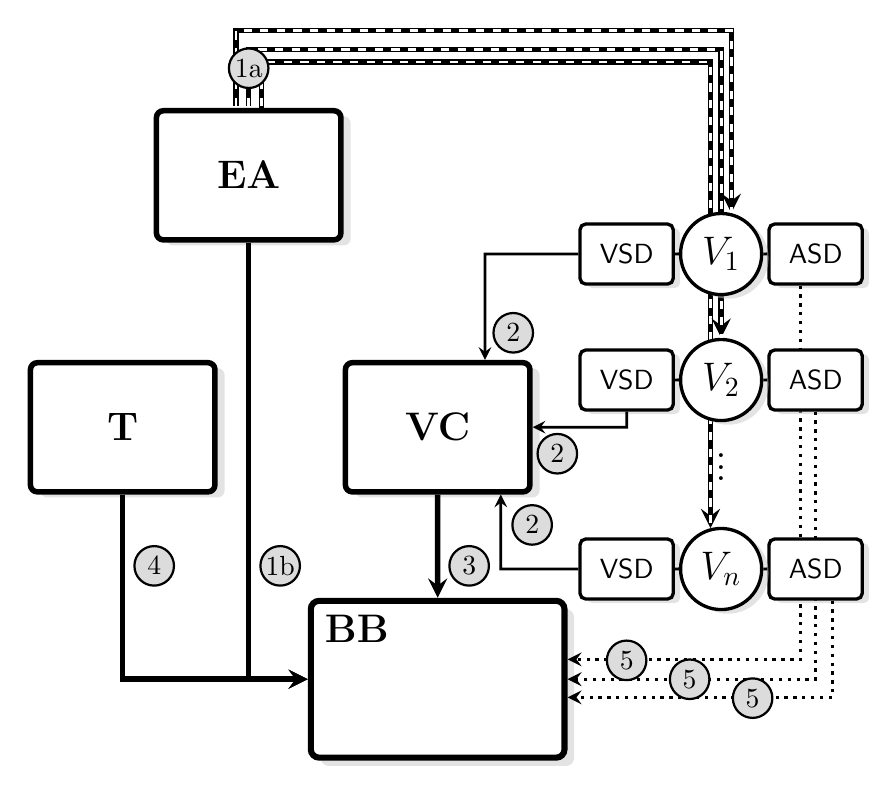
\begin{tikzpicture}[scale=0.8]
  %\draw[step=10pt,gray,very thin] (0,0) grid (30,30);
  
  %\draw[step=1pt,thick] (25,15) rectangle (28,16.5) ;
  \node[draw, align = center, text width = 60pt, text height=40pt,rounded corners=2.5pt,line width=2pt,fill = white, drop shadow={shadow xshift=3.5pt, shadow yshift=-2pt, fill=mygray}]  (EA) at (7,24) {};
  
    \node[draw, align = center, text width = 60pt, text height=40pt,rounded corners=2.5pt,line width=2pt,fill = white, drop shadow={shadow xshift=3.5pt, shadow yshift=-2pt, fill=mygray}]  (VC) at (10,20) {};
    
      \node[draw, align = center, text width = 60pt, text height=40pt,rounded corners=2.5pt,line width=2pt,fill = white, drop shadow={shadow xshift=3.5pt, shadow yshift=-2pt, fill=mygray}]  (T) at (5,20) {};
    
  \node at (EA) {\Large{\textbf{EA}}};
 \node at (VC) {\Large{\textbf{VC}}};
  \node at (T) {\Large{\textbf{T}}};
%



 %
% \node (CD) at (11,23.5) {};

 
\node[draw, fill =white, align = center, text width = 85pt,text height=50pt,rounded corners=3pt,line width=2.2pt, drop shadow={shadow xshift=3.5pt, shadow yshift=-3pt, fill=mygray}] (BB) at (10,16) {}; 

 \node[below right, inner sep=6pt] at (BB.north west) {\Large{\textbf{BB}}};
 
  \draw[->,>=stealth,line width=2pt] (VC)--(BB) ;
    \draw[->,>=stealth,line width=2pt] (EA.south) |- (BB.west);
    \draw[->,>=stealth,line width=2pt] (T.south) |- (BB.west);

 
 %
  \node[SD](VSD1) at (13,22.75) {};
        \node[SD](VSD2) at (13,20.75) {};
     \node[SD](VSDn) at (13,17.75) {};
   
      \node[SD](V-ASD1) at (16,22.75) {};
   \draw[->,>=stealth,dotted,very thick] ([xshift=-80pt]V-ASD1)|-([yshift=25pt]BB);
      \node[SD](V-ASD2) at (16,20.75) {};     
      \draw[->,>=stealth,dotted, very thick] (V-ASD2)|-(BB);      
           \node[SD](V-ASDn) at (16,17.75) {};
         \draw[->,>=stealth,dotted, ,very thick] ([xshift=40pt]V-ASDn)|-([yshift=-25pt]BB);
         
         
     \node[align = center, text width = 22pt, thick]  (Vdots) at (14.5,19.5) {\Large{$\vdots$}}  ; 
     %
         %
    \node[human]  (Vn) at (14.5,17.75) {\Large{$V_n$}}  ;      
   \node at (VSDn) {{\textsf{VSD}}};
   \node at (V-ASDn) {{\textsf{ASD}}};
   \draw[->,>=stealth,line width=2pt] (7.2,25)--(7.2,25.8) -|([xshift=-60pt]Vn) ;
 \draw[-,>=stealth,dashed,line width=1pt,color=white] (7.2,25.1)--(7.2,25.8) -|([xshift=-60pt,yshift=-25pt]Vn) ;

         %         
    \node[human]  (V2) at (14.5,20.75) {\Large{$V_2$}}  ; 
   \node at (VSD2) {{\textsf{VSD}}};
   \node at (V-ASD2) {{\textsf{ASD}}};
  \draw[->,>=stealth,line width=2pt] (7,25.1)--(7,26) -|(V2) ;
    \draw[-,>=stealth,dashed,line width=1pt,color=white] (7,25.1)--(7,26) -|([yshift=-25pt]V2) ;
%         
   \node[human]  (V1) at (14.5,22.75) {{\Large{$V_1$}}}  ; 
   \node at (VSD1) {{\textsf{VSD}}};  
   \node at (V-ASD1) {{\textsf{ASD}}};
   \draw[->,>=stealth,line width=2pt] (6.8,25.1)--(6.8,26.3) -|([xshift=25pt]V1) ;
  \draw[-,>=stealth,dashed,line width=1pt,color=white] (6.8,25.1)--(6.8,26.3) -|([xshift=25pt,yshift=-25pt]V1) ;

 %

   %
\draw [->,>=stealth,line width=1pt] (V-ASD1)--(V1) -- (VSD1)-|([xshift=55pt]VC) ;
\draw [->,>=stealth,line width=1pt] (V-ASD2)--(V2) -- (VSD2)|-(VC) ;
\draw [->,>=stealth,line width=1pt] (V-ASDn)--(Vn)-- (VSDn)-|([xshift=60pt]VC) ;

 \node[draw,circle,text width=6pt,line width=0.8pt,fill = lightgray] (C1b) at (7.5,17.8) {};
 \node at (C1b) {1b} ;
 %
  \node[draw,circle,text width=6pt,line width=0.8pt,fill = lightgray] (C1a) at (7,25.7) {};
 \node at (C1a) {1a} ;
 %
  \node[draw,circle,text width=6pt,line width=0.8pt,fill = lightgray] (C3) at (5.5,17.8) {};
 \node at (C3) {4} ;
  %
  \node[draw,circle,text width=6pt,line width=0.8pt,fill = lightgray] (C2b) at (10.5,17.8) {};
 \node at (C2b) {3} ;
 %
  \node[draw,circle,text width=6pt,line width=0.8pt,fill = lightgray] (C41) at (13,16.3) {};
 \node at (C41) {5} ;
 %
  \node[draw,circle,text width=6pt,line width=0.8pt,fill = lightgray] (C42) at (14,16) {};
 \node at (C42) {5} ;
 %
  \node[draw,circle,text width=6pt,line width=0.8pt,fill = lightgray] (C4n) at (15,15.7) {};
 \node at (C4n) {5} ;
 
   \node[draw,circle,text width=6pt,line width=0.8pt,fill = lightgray] (C21) at (11.2,21.5) {};
 \node at (C21) {2} ;
 %
  \node[draw,circle,text width=6pt,line width=0.8pt,fill = lightgray] (C22) at (11.9,19.58) {};
 \node at (C22) {2} ;
 %
  \node[draw,circle,text width=6pt,line width=0.8pt,fill = lightgray] (C2n) at (11.5,18.45) {};
 \node at (C2n) {2} ;
\end{tikzpicture}
    \caption{The interaction among the entities in an e-voting execution. The dotted lines denote read-only access to the BB. The dashed arrows denote channels for voters' private inputs distribution. Annotation: (1a): distribution of voter's private inputs; (1b): posting pre-election BB data; (2): vote casting; (3): writing votes to BB; (4) posting post-election BB data and the election results; (5): auditing.}
        \label{interaction}
\end{figure}
An e-voting system $\Pi$ is a quintuple of algorithms and protocols  \textbf{(Setup, Cast, Tally, Result, Verify)}, that takes  voters' preferences as an input and aims to return a tally, the protocols specified as follows:
\begin{enumerate}
\item The interactive protocol \textbf{Setup} is executed by the $\ea$ and $\T$. During the setup phase, $\ea$ generates $\Pi$'s public parameters $Pub$ (which include $P, V, U$) and the voters' secrets $s_1, \dots , s_n$. The part of the interactive protocol during which $\ea$ distributes secrets among voters is defined as \textbf{Registration}. At the same time, $\T$ generates pre-election $\bb$ data and posts it on $\bb$.
\item The interactive protocol \textbf{Cast} is executed between three parties, the voter $V_l$, the $\bb$ and the $\voc$. During this interaction, the voter uses $\vsd$, his secret $s_l$ and an option $U_l$ to generate the ballot $b_l$ and sends this ballot to $\voc$. Upon successful termination, $\voc$ posts ballot $b_l$ to $\bb$ and the voter $V_l$ receives a receipt $\alpha_l$.
\item The interactive protocol \textbf{Tally}\fix{}{You have forgotten to write Tally.}
\item The algorithm \textbf{Result} is executed by $\T$ and outputs the result $\tau$ for the election or returns $\perp$ if result is undefined.
\item  The algorithm \textbf{Verify} on input $\alpha,\tau$ outputs a bit that determine whether the verification was successful or not.  $\alpha$ is a voter receipt obtained after the \textbf{Cast} protocol execution.
\end{enumerate}
In some e-voting systems \textbf{Registration} part is omitted and voters are expected to receive their credentials via a secure channel such as post mail, polling place etc.
\begin{definition}[Correctness of e-voting system by Kiayias et al. \cite{Kiayias2015}]
It is said that a system $\Pi$ has (perfect) correctness, if for any honest execution of any subset of not abstained voters that results in a public transcript $\tau$, where the voters $V_1, . . . , V_n$ cast votes for options $U_1, . . . , U_n$, it holds that $Result(\tau) = f(U_1,...,U_n)$, where $f(U_1,...,U_n)$ is the m-vector \fix{whose}{which} i-th location is equal to the number of times a candidate $P_i \in \{P_1,\dots, P_m\}$ was chosen in the candidate selections $U_1, . . . , U_n$.
\end{definition}
\section{Election process}
Any electronic voting procedure can be split into three general stages: Pre-election, Election and Post-election. For some specific e-voting schemes, the first or the last stage can be omitted.\fix{}{I can not see how you can completely eliminate Setup (pre-election) or Tally (post-election}
\begin{enumerate}
\item Pre-election: $\ea$ generates public pre-election data and posts it on the $\bb$. Also, $\ea$ creates and distributes envelopes with private voters' information among all eligible voters. Meanwhile, $\T$ obtains secret data that would be used for producing the result and posts its own pre-election data to the $\bb$.
\item Election: this stage typically is split into two parts:
\begin{enumerate}
\item Registration: A voter and $\ea$ engaged in an interaction during which the voter proofs to the $\ea$ his identity and obtains credentials for vote casting. In some e-voting systems, the registration part is omitted, and voters receive their credentials in envelopes via some secure channel. 
\item Vote casting: A voter starts an interaction with $\vsd$ using his credentials as proof of his eligibility to cast a vote for preferred candidates. Upon successful termination, $\voc$ receives a ballot from $\vsd$ and posts it on the $\bb$. 
\end{enumerate}
\item Post-election: After the election is closed, the election result is computed and announced by $\T$.  If verification is supported, anyone may check the validity of the election procedure. 
\end{enumerate}

\section{E2E Verifiability}
\label{e2e}
E2E verifiability is a very strong level of security that allows voters  to detect that a malicious e-voting system tries to misrepresent the election outcome. Three aspects of verifiability are usually distinguished:
\begin{enumerate}
\item \textit{Individual verifiability}: a voter can check that his ballot is counted correctly \cite{Chaum1981}.
\item \textit{Universal verifiability}: anyone can check that the election outcome is obtained from the ballots published on the $\bb$ \cite{Sako1995}.
\item \textit{End-to-end verifiability}: a voter can check that his vote was cast-as-intended and recorded-as-cast, also anyone can check that the ballots were tallied-as-recorded \cite{Neff2004},\cite{Chaum2004}.
\end{enumerate}

 In this work, we use the E2E-verifiability definition by Kiayias et al. \cite{Kiayias2015a},\cite{Kiayias2015}, \fix{the definition is listed}{which is presented} in Figure \ref{sec:e2e}. 
According to the definition, an adversary $\mathcal{A}$ can control all $\vsd$'s, $\ea$, $\voc$ and some fraction of voters, however, it still can not manipulate the results without a high detection probability.  The entities involved are $\bb$, $\vsd$ and $\ea$ that can be split on $\ea$, that involved on pre-election stage only, and $\T$ that computes the results. The algorithm \textbf{Cast} is run interactively between tree parties the $\bb$, the voter $V_l$ and $\T$ that uses $\vsd$ with the following inputs: public parameters $Pub$, voter's secret $s_l$ and voter's choice $\mathcal{U}_l$. Upon successful termination, $V_l$ obtains a receipt $\alpha_l$. The algorithm \textbf{Verify}($\tau,\alpha_l$) outputs a bit, based on voter's receipt $\alpha_l$ and the public transcript $\tau$. The algorithm \textbf{Result}($\tau$) given the public transcript $\tau$  outputs the result for the election or $\bot$ if the result is undefined.\\
\begin{figure}[h!]
 \fbox{\parbox{\textwidth}{
\underline{ E2E Verifiability Game $G^{\mathcal{A},\mathcal{E},d,\theta}_{E2E-Ver}(1^{\lambda},m,n)$}:
\begin{enumerate}
\item  $\mathcal{A}$ chooses a list of candidates $\mathcal{P} = \{P_1,\dots,P_m\}$, a set of voters $\mathcal{V} = \{V_1,\dots,V_n\}$ and the set of allowed candidate selections $\mathcal{U}$. It provides $\mathcal{C}$ with the sets $\mathcal{P}$,$\mathcal{V}$,$\mathcal{U}$ along with information $Pub$ and voter credentials $\{s_{l \in [n]}\}$. Throughout the game, $\mathcal{C}$ plays the role of the $\bb$.
\item  The adversary $\mathcal{A}$ and the challenger $\mathcal{C}$ engages in an interaction where  $\mathcal{A}$ schedules the \textbf{Cast} protocols of all voters. For each voter $V_l$  $\mathcal{A}$ can either completely control the voter or allow $\mathcal{C}$ to operate on their behalf, in which case $\mathcal{A}$ provides a candidate selection $\mathcal{U}_l$ to $\mathcal{C}$. Then, $\mathcal{C}$ engages with the adversary $\mathcal{A}$ in the \textbf{Cast} protocol so that  $\mathcal{A}$ plays the role of $\ea$. Provided the protocol terminates successfully, $\mathcal{C}$ obtains the receipt $\alpha_l$ on behalf of $V_l$.\\
 Let $\tilde{\mathcal{V}}$ be the set of honest voters (i.e., those controlled by $\mathcal{C}$) that terminated successfully. 
\item Finally, $\mathcal{A}$ posts the election transcript $\tau$ to the $\bb$.
\end{enumerate}
The game returns a bit which is 1 if and only if the following conditions hold true: \\
(i)  $|\tilde{\mathcal{V}}| \geq \theta$, (i.e., at least $\theta$ honest voters terminated).\\
(ii). $\forall l \in  [n]$: if $V_l \in  \tilde{\mathcal{V}}$, then \textbf{Verify}($\tau,\alpha_l$)=1 (i.e., the voters in $\tilde{\mathcal{V}}$ verify their ballot successfully).\\
and either one of the following two conditions: \\
~~~~(iii-a). If $\bot \ne \rangle \mathcal{U}_l \rangle _{V_l \in \mathcal{V}\setminus \tilde{\mathcal{V}}} \leftarrow \mathcal{E}(\tau, \{\alpha_l\} _{V_l \in   \tilde{\mathcal{V}}})$,\\
~~~~~~~then $d_1$(\textbf{Result}($\tau$),$f(\langle U_1,\dots,U_n \rangle)) \geq d$. \\
~~~~(iii-b). $\bot \leftarrow \mathcal{E}(\tau, \{\alpha_l\} _{V_l \in   \tilde{\mathcal{V}}})$.
 }}
\caption{E2E-verifiability by Kiayias et al.}
 \label{sec:e2e}
 \end{figure}
 We prefer the definition by Kiayias et al over the one given by K\"{u}sters et al \cite{Kusters2010}, because it is given in game-based settings. Moreover, this definition of E2E Verifiability does not require any additional assumptions, except for the existence of the $\bb$, therefore it is achievable in the standard model. Furthermore, there is an ideal functionality that captures the essential aspects of the E2E Verifiability \cite{idfunc}.  \thomas{This is comparison is not correct. We can discuss about it}
 
 \section{The Universal Composability Framework}
 \label{uc}
The Universal Composability (UC) is a framework for representing cryptographic protocols and analysing their security \cite{Canetti2001}. UC provides very  strong security guarantees and allows to specify security requirements in a unified and systematic way. There are just tree entities involved: a protocol, an adversary and an environment that captures everything else that goes beyond the protocol execution. The best explanation what does UC mean is given by Jens Groth: "In the UC framework, an execution of a multi-party computation protocol is compared to an execution where a trusted ideal functionality handles the data and produces the output. A protocol is said to be secure if an adversary operating in a real-life model can be simulated in the ideal process model with the ideal functionality. In the case of voting, the ideal functionality takes as input the votes and outputs the result of the election. This ideal functionality corresponds to the old method of voters marking their choice on paper and putting the ballot in a box, which is opened once the election is over."\cite{Groth2004}.\\

Originally UC considers the execution of an unbounded number of concurrent protocols in the arbitrary environment, controlled by an adversary. Even though UC seems to be the most realistic level of security, it cannot be achieved in general without some trusted setup assumptions \cite{Lin2009}. The stand-alone setting on the other hand only allows the execution of a single instance of the protocol at a time and guarantees the security under sequential composition, namely if a protocol is secure in the stand-along model it maintains its security in sequential runs, where each execution concludes before the next one begins.  Sequential composition does not imply security in the concurrent composition, however, it provides reasonably high-security guarantees.\\ 

In the stand-alone model, an adversary is restricted from communicating with the environment during the protocol execution. The stand-alone model enables one to design a protocol using calls to an ideal functionality, which is secure by design,  and check whether a real protocol properly implements this ideal protocol. This makes security analysis significantly more simple. A protocol is said to be secure if, for all adversaries, there exists a simulator so that real and ideal executions are indistinguishable for and any environment \cite{Lindell2016}. \fix{}{I do not see the reason to include UC as a big separate section. In addition, one can not exclude the feasibility of UC security assuming a consistent BB.}
\section{Random Oracle}
\label{rom}
Random Oracle Model was invented as an artificial  way to construct formal security proofs for certain types of cryptographic protocols \cite{Bellare1993}. The model can be described as a black box with a perfectly random function we know nothing about . We can input some new date into the box (ask quires) and receive an uniformly distributed random output. However, if given an already seen input, the box outputs whatever it returned the last time. \\

Basically, Random Oracle is an perfect hash function i.e. a \textit{random function} with memory. Unfortunately, random functions are impractical -- it is just an model, that can not be implemented in the real life. There exist signature and encryption schemes that are secure in the Random Oracle Model, but for which any implementation of the random oracle results in insecure schemes. Therefore, for constructing security proofs in Random Oracle model, we pretend that some real implementation of the hash function is perfectly random, even though it is decidedly not random. The problem with this approach is that it is unclear what security guarantees it buy us in the real world. Canetti et al. \cite{Canetti2004} prove that there are protocols that secure in Random Oracle model, but any implementation of such protocols results in insecure schemes. \fix{However, despite everything}{Despite this negative result}, security proofs in Random Oracle model are much better than no proofs at all and this model was wildly used for proving security of RSA, ElGamal etc.\fix{In addition, the Random Oracle model often yields to more efficient constructions, applicable in real-world scenarios.}\\

Definitions are given in the Standard and Random Oracle models are incomparable. The Standard model implies that security relies on the standard cryptographic assumptions, while in Random Oracle we assume that our implementation of the hash function is perfectly random, even thought it is not. 
%% This is an example first chapter.  You should put chapter/appendix that you
%% write into a separate file, and add a line \include{yourfilename} to
%% main.tex, where `yourfilename.tex' is the name of the chapter/appendix file.
%% You can process specific files by typing their names in at the 
%% \files=
%% prompt when you run the file main.tex through LaTeX.
\chapter{Privacy}

Voter privacy implies that a voter is capable of casting his own vote secretly and freely without letting others' parties, namely an adversary, to learn some information about his preferences or interfere in it.\\

In general, the goal of the adversary who attacks voter privacy is to learn some information about the candidate selections of the honest voters. Similarly to \cite{Kiayias2015}, we define an attack against voters privacy as successful, if there is an election result*, for which an adversary is capable of distinguishing how the honest voters voted while it can observe the whole e-voting network, except for untrappable channels, and corrupt some part of honest voters and some entities and also has access to honest voters' receipts. \\

*Obviously, it doesn't include trivial election results, where all voters voted for the same option. \\

During the election process, a voter uses his credentials to cast a vote for some option by running the \textbf{Cast} protocol on a $\vsd$. Since voters are not allowed to have or share a secret that would have helped them to preserve their privacy in case of a corrupted e-voting system, their privacy relies on the trusted entities of the system. There are two wildly known classes of e-voting systems: code-based system and encryption-based systems. The former relies on crypto that is run by the trusted administrator in advance, the latter places its safety on crypto performed inside $\vsd$ during the \textbf{Cast} protocol execution. From a voter point of view, it means that his privacy is protected by trusted administrator and pre-calculated credentials, that would not reveal any sensitive information even if the choice is sent in a plain text, or by trusted $\vsd$ and crypto performed inside it. \\

The approach that we used in this thesis is the following: an honest voter is allowed to have  \textbf{only one} perfectly hidden from an adversarial eyes interaction and at the end, he provides the adversary with the real and simulated view of the result of this interaction. $\mathcal{A}$ is allowed to observe a network trace of all interactions and play on behalf of corrupted entities and voters. This one perfectly private interaction can be either an act of actually entering voter's preference into $\vsd$ or while a voter receives his credentials. If $\mathcal{A}$  has no advantage in distinguishing real and simulated view over a coin flip, the system is considered private. \\

We formally define the voter privacy via a Voter Privacy game, denotes as $G_{t-priv,<honest~entities>}^{\mathcal{A}, Sim}(1^{\lambda})$, that is played between an adversary $\mathcal{A}$ and a challenger $\mathcal{C}$, that takes as input the security parameter $\lambda$ and returns 1 or 0 depending on whether the adversary wins.  Also, $\mathcal{A}$ is  allowed to corrupt some entities. The choice of the corrupted parties splits the Voter Privacy game into two different scenarios: (1) entities ($\ea$, $\T$) are honest and (2) $\vsd$ is honest. \\

 \section{$\ea$ and $\T$ are honest: $G_{t-priv,\ea,\T}^{\mathcal{A}, Sim}(1^{\lambda})$}
  \begin{figure}
 \includestandalone[mode=buildnew]{figures/figure1}
        \caption{  $G_{t-priv,\ea,\T}^{\mathcal{A}, Sim}(1^{\lambda},n,m)$}
\end{figure}our 

The $\mathcal{C}$'s strategy  in the  $G_{strict,\ea,\T}^{\mathcal{A}, Sim}(1^{\lambda},n,m)$ game captures the ability of an honest voter to lie about his vote in code-based e-voting schemes. Suppose, an adversary $\mathcal{A}$ makes a voter $V$ to vote for an option $U_{\mathcal{A}}$.  However, $V$ disobeys and votes for his intent $U_{V}$. If $V$ can fake his credentials  and convince $\mathcal{A}$ that he voted for $U_{\mathcal{A}}$, $V$'s privacy is preserved. This approach is similar to \textit{Demos Privacy} \cite{Kiayias2015}, however instead of faking voter's internal view of the \textbf{Cast} protocol, we fake credentials in a way that would produce a fake internal view of the \textbf{Cast} protocol.\\

We compare \textit{Demos Privacy} and the \textit{Voter Privacy} defined here as follows. Under \textit{Demos Privacy} framework a voter $V$ provides $\mathcal{A}$  with a fake internal view of the \textbf{Cast} protocol and the actual receipt as a proof of obedience but keeps the original credentials in secret. If $\mathcal{A}$ accesses the voter's original credentials, it would immediately detect the lie. Under our \textit{Voter Privacy} definition, a voter $V$ gives $\mathcal{A}$ a fake view, actual receipt and fake credentials. If $\mathcal{A}$ can not distinguish real and fake credentials, it has no way to find out whether $V$ lies or not. \\
 
In the game $G_{t-priv,\ea,\T}^{\mathcal{A}, Sim}(1^{\lambda},n,m)$, an adversary $\mathcal{A}$ interacts with the challenger $\mathcal{C}$ on behalf of all corrupted voters, $\voc$ and $\vsd$. $\mathcal{C}$ plays the role of honest voters, $\ea$ and $\T$. $\bb$ is completely passive and represents a publicly viewed database. \\

 1)  $\mathcal{A}$ picks and sends two options $U_i^0,U_i^1$ to the challenger $\mathcal{C}$. The first option $U_i^0$ is its intent, the other -- the option that the challenger would use in order to produce an indistinguishable from the intent's ballot and receipt view*. 2) After sending options, $\mathcal{A}$ schedules the   \textbf{Registration} protocol with $\mathcal{C}$ on behalf of some voter $V_i$. 3) $\mathcal{C}$ creates fake credentials $\tilde{s_i}$ and generates real credentials $s_i$ for the voter $V_i$. 4) $\mathcal{C}$ responds $\mathcal{A}$ with a pair of credentials $s_i^0,s_i^1$, where one of the credentials are real and the other were generated using the simulator $Sim$ in a such way, that if $\mathcal{A}$ guesses right and uses the real credentials to cast a vote for $U_i^0$, the produced ballot and internal view of the \textbf{Cast} protocol would be real, otherwise generated ballot would correspond to the option $U_i^1$ and the returned view would be fake. 5) If $\mathcal{A}$ chooses to post the ballot $b_i$ to $\bb$, 6) $\mathcal{C}$  posts exactly the same ballot** to $\bb$. 7) When $\mathcal{A}$ stops the election, $\mathcal{C}$ posts the tally $\tau$ ***. \\\\
\textit{Remarks}:\\
Denote the list of honest voters for which $\mathcal{A}$ chooses to post produced ballot and uses credentials $s_i^0$  as $ \tilde{\mathcal{V}}^0$ and the similar list but for credentials $s_i^1$ as $ \tilde{\mathcal{V}}^1$. \\\\
*If  $\mathcal{C}$ succeeds, $\mathcal{A}$ wouldn't be able to say whether it voted for option $U_i^0$ or $U_i^0$ and $\bb$ would contain both ballots (one for the option $U_i^0$ ,the other for the option $U_i^1$) so the tally wouldn't reveal any information. Example: if $\mathcal{A}$  picks real credential then it casts a vote for the option  $U_i^0$ on behalf of a voter $V_i$, at the same time exactly the same ballot posted by $\mathcal{C}$ would correspond to the fake credentials and the option $U_i^1$. In this case, $\mathcal{A}$ indeed voted for $U_i^0$ as it intended. Else if $\mathcal{A}$ picks the fake credentials and votes for the option $U_i^0$,  its ballot corresponds to the real credentials and  the option $U_i^1$. At the same time, exactly the same ballot posted by $\mathcal{C}$ corresponds to the fake credentials  and the option $U_i^0$. In the last case $\mathcal{A}$ actually voted for $U_i^1$ while thinking it casts vote for $U_i^0$. If this privacy holds,  $\mathcal{A}$ has no idea what option voter $V_i$ voted for. \\\\
** $\mathcal{C}$ should post to the $\bb$ a ballot for the remaining candidate and since $\mathcal{C}$ does not control $\vsd$, it can only post the identical ballot, but \textbf{Tally} it as if it was generated with fake credentials. If  $\mathcal{A}$  voted for $U_i^0$, $\mathcal{C}$ should vote for the $U_i^1$ and vice versa. Otherwise  $\mathcal{A}$  would guess the coin $a$ by simply checking the result of an election. $\mathcal{A}$ is allowed to pick any two options $U_i^0,U_i^1$  and play as many rounds as it likes. Since lists $\langle \mathcal{U}^0_i \rangle _{V_i \in \tilde{\mathcal{V}}^0} $ and  $\langle \mathcal{U}^1_i \rangle _{V_i \in \tilde{\mathcal{V}}^1} $  not necessarily produce the same result as lists  $\langle \mathcal{U}^0_i \rangle _{V_i \in \tilde{\mathcal{V}}^1} $ and  $\langle \mathcal{U}^1_i \rangle _{V_i \in \tilde{\mathcal{V}}^0} $, the adversary would trivially break privacy. To prevent this, we add challenger's ballots to the $\bb$ and compute the combined tally, namely $f(\langle \mathcal{U}^0_i \rangle _{V_i \in \tilde{\mathcal{V}}^0} ) + f(\langle \mathcal{U}^1_i \rangle _{V_i \in \tilde{\mathcal{V}}^0} )+ f(\langle \mathcal{U}^0_i \rangle _{V_i \in \tilde{\mathcal{V}}^1} ) +  f(\langle \mathcal{U}^1_i \rangle _{V_i \in \tilde{\mathcal{V}}^1} )$. However, if lists $\langle \mathcal{U}^0_i \rangle _{V_i \in \tilde{\mathcal{V}}^0}, \langle \mathcal{U}^1_i \rangle _{V_i \in \tilde{\mathcal{V}}^1}$ and $\langle \mathcal{U}^1_i \rangle _{V_i \in \tilde{\mathcal{V}}^0}, \langle \mathcal{U}^0_i \rangle _{V_i \in \tilde{\mathcal{V}}^1}$ sums to the same result $f(\langle \mathcal{U}^0_i \rangle _{V_i \in \tilde{\mathcal{V}}^0} ) + f(\langle \mathcal{U}^1_i \rangle _{V_i \in \tilde{\mathcal{V}}^1} ) =  f(\langle \mathcal{U}^0_i \rangle _{V_i \in \tilde{\mathcal{V}}^1} ) +  f(\langle \mathcal{U}^1_i \rangle _{V_i \in \tilde{\mathcal{V}}^0} )$, we remove the challenger's ballots  and compute the actual tally. \\\\
*** The tally $\tau$ is posted only if, for every correctly formed adversarial ballot, there is a corresponding challenger's ballot posted on the $\bb$. $\mathcal{A}$ may not post some ballots, however, if it does, then the corresponding challenger's ballot must be posted as well. Otherwise, $\mathcal{A}$ wins the \textit{Voter Privacy} game by simply checking the announced result.  All $\mathcal{A}$'s ballots are tallied based on real credentials, all  $\mathcal{C}$'s ones -- based on fake credentials.   $\mathcal{C}$ removes all its  ballots and computes tally for the adversarial ballots if and only if  lists $\langle \mathcal{U}^0_i \rangle _{V_i \in \tilde{\mathcal{V}}^0}, \langle \mathcal{U}^1_i \rangle _{V_i \in \tilde{\mathcal{V}}^1}$ and $\langle \mathcal{U}^1_i \rangle _{V_i \in \tilde{\mathcal{V}}^0}, \langle \mathcal{U}^0_i \rangle _{V_i \in \tilde{\mathcal{V}}^1}$ are summed up to the same result i.e. $f(\langle \mathcal{U}^0_i \rangle _{V_i \in \tilde{\mathcal{V}}^0} ) + f(\langle \mathcal{U}^1_i \rangle _{V_i \in \tilde{\mathcal{V}}^1} ) =  f(\langle \mathcal{U}^0_i \rangle _{V_i \in \tilde{\mathcal{V}}^1} ) +  f(\langle \mathcal{U}^1_i \rangle _{V_i \in \tilde{\mathcal{V}}^0} )$. In this case, the announced tally would be $f(\langle \mathcal{U}^0_i \rangle _{V_i \in \tilde{\mathcal{V}}^0} ) + f(\langle \mathcal{U}^1_i \rangle _{V_i \in \tilde{\mathcal{V}}^1} )$ if challenger's coin $a=0$ or  $f(\langle \mathcal{U}^0_i \rangle _{V_i \in \tilde{\mathcal{V}}^1} ) +  f(\langle \mathcal{U}^1_i \rangle _{V_i \in \tilde{\mathcal{V}}^0} )$ otherwise.\\

 $G_{t-priv,\ea,\T}^{\mathcal{A}, Sim}(1^{\lambda},n,m)$ defined as follows:\\
\begin{enumerate}
\item $\mathcal{A}$ on input $1^{\lambda},n,m$ defines a set of voters  $\mathcal{V} = \{V_1,...,V_n\}$, chooses a list of candidates  $\mathcal{P} = \{P_1,...,P_m\}$ and the set of allowed candidates' selections $\mathcal{U}$.  It provides $\mathcal{C}$ with $\mathcal{V}, \mathcal{P}, \mathcal{U}$.
\item $\mathcal{C}$ flips a coin $a \leftarrow \{0,1\}$ to define an order according to which real and simulated credentials would be returned to $\mathcal{A}$, and starts the election on behalf of $\ea$. 
\item The adversary $\mathcal{A}$ picks two option $U^0_i,U^1_i \in \mathcal{U}$, where $U^0_i$ is its intent and $U^1_i$ is an option that $\mathcal{C}$ would use in order to fool $\mathcal{A}$.  After that, $\mathcal{A}$  and $\mathcal{C}$ engage in an interaction where $\mathcal{A}$ schedules the \textbf{Registration} protocols, during which all voters receive their credentials and forward them to  $\mathcal{A}$. For each voter $V_i \in \mathcal{V}$, the adversary chooses whether $V_i$ is corrupted:
\begin{enumerate}
\item[] -- If $V_i$ is corrupted, then $\mathcal{C}$ provides $\mathcal{A}$ with the real credentials $s_i$, and then they engage in a \textbf{Cast} protocol where the $\mathcal{A}$  vote on behalf of $V_i$ and  $\mathcal{C}$ plays the role of $\ea$.
\item[] --  If $V_i$ is not corrupted, then $\mathcal{C}$ generates real credentials $s_i$  and fake credentials $\tilde{s_i}$ using $Sim$.  $\mathcal{C}$  responds  $\mathcal{A}$ with a pair of simulated and real credentials $(s_0,s_1)$ in order defined by the coin a:\\
$ \begin{cases}
 \text{if} ~~a =0,~~ (s^0_i,s^1_i) = (\tilde{s_i},s_i)  \\ 
 \text{else}~~  (s^0_i,s^1_i) = (s_i,\tilde{s_i})
\end{cases}$
 \item[] -- An honest voter $V_i$ forwards both credentials $s^0_i,s^1_i$ to $\mathcal{A}$
\item[] -- Using one of the credentials $\mathcal{A}$ schedules the \textbf{Cast} protocol execution to vote for an option $U^0_i$ and sends the produced ballot to $\bb$ in the entry that corresponds to the voter $V_i$. As a result of the \textbf{Cast} protocol execution, $\mathcal{A}$ would obtain receipt $r_i$, ballot $b_i$ and the view of the internal state of the voter $V_i$ $view_i$.  During the \textbf{Tally} protocol execution this ballot would be treated as if it was generated with real credentials $s_i$. So, if  $\mathcal{A}$ indeed picked the real credentials, $b_i$ would correspond to the option   $U^0_i$  and $view_i$ would be real. Otherwise, $b_i$ would be a ballot for the option  $U^1_i$ and $view_i$ would be fake. 
\item[] --  If  $\mathcal{A}$ posts a ballot on $\bb$, $\mathcal{C}$ posts exactly the same ballot. During the \textbf{Tally} protocol execution, this ballot would be treated as if it was generated with fake credentials, which means that whatever option in reality $\mathcal{A}$ voted for, $\mathcal{C}$ picked the other option.  
\end{enumerate}
\item Denote the list of honest voter for which $\mathcal{A}$ chooses to post produced ballot and uses credentials $s_i^0$  as $ \tilde{\mathcal{V}}^0$ and the similar list but for credentials $s_i^1$ as $ \tilde{\mathcal{V}}^0$.  If  lists $\langle \mathcal{U}^0_i \rangle _{V_i \in \tilde{\mathcal{V}}^0}, \langle \mathcal{U}^1_i \rangle _{V_i \in \tilde{\mathcal{V}}^1}$ and $\langle \mathcal{U}^1_i \rangle _{V_i \in \tilde{\mathcal{V}}^0}, \langle \mathcal{U}^0_i \rangle _{V_i \in \tilde{\mathcal{V}}^1}$ are summed up to the same result i.e. $f(\langle \mathcal{U}^0_i \rangle _{V_i \in \tilde{\mathcal{V}}^0} ) + f(\langle \mathcal{U}^1_i \rangle _{V_i \in \tilde{\mathcal{V}}^1} ) =  f(\langle \mathcal{U}^0_i \rangle _{V_i \in \tilde{\mathcal{V}}^1} ) +  f(\langle \mathcal{U}^1_i \rangle _{V_i \in \tilde{\mathcal{V}}^0} )$, $\mathcal{C}$ removes all its ballots and executes the \textbf{Tally} protocol on the cleared $\bb$ with real credentials. Otherwise, $\mathcal{C}$ executes the \textbf{Tally} protocol on the $\bb$ that contains both adversarial and challenger's ballots and uses real credentials for adversarial ballots and fake ones for its own. 
\item Finally, $\mathcal{A}$ using all information collected above (including the contents of the BB) outputs a bit $a^*$
\item Denote the set of corrupted voters as $\mathcal{V}_{corr}$ and the set of honest voters as $\hat{\mathcal{V}}= \mathcal{V} \backslash \mathcal{V}_{corr}$. The game returns a bit which is 1 if and only if the following hold true:
\begin{enumerate}
 \item $a = a^*$
 \item $|\mathcal{V}_{corr}| \leq t$ (i.e., the number of corrupted voters is bounded by $t$).
\end{enumerate} 
\end{enumerate}

\textbf{Remark:}\\
$Sim$ works in such a way that fake credentials satisfy both of the following rules: 
\begin{enumerate}
 \item The real credentials and $U_i^0$ option  should give ballot and receipt, which are identical to ballot and receipt produced for the fake credentials and  $U_i^1$ option.
 \item The fake credentials and $U_i^0$ option  should give ballot and receipt, which are identical to ballot and receipt produced for the real credentials and  $U_i^1$ option.
 \end{enumerate}

To understand the logic behind the \textit{Voter Privacy} defined above, consider the following toy examples.\\\\
\textbf{Example 1}\\
We have three voters $V_1,V_2,V_3$ and three possible options $op_1,op_2,op_3$. Challenger's coin $a=0$, so, during the game, the fake credentials are always the first credentials in the credentials pair.
Suppose  $\mathcal{A}$' schedules three vote casting protocols for voters $V_1,V_2,V_3$: \\\\
1)$\boxed{V_1}$:  $\mathcal{A}$ chooses $U^0_1 = op_3, U^1_1 = op_1$ and picks the second credentials for generating the ballot $b_1$ for $op_3$. Since  $\mathcal{A}$ picked the real credentials, the ballot $b_1$ in the \textbf{Tally} process would correctly result in a vote for $op_3$. Meanwhile, $\mathcal{C}$ posts identical to the ballot $b_1$ ballot $\tilde{b_1}$ that corresponds to an option $op_1$.\\
2)$\boxed{V_2}$: $\mathcal{A}$ chooses $U^0_2 = op_1, U^1_2 = op_2$ and picks the first credentials for generating the ballot $b_2$ for $op_1$. Since  $\mathcal{A}$ picked the fake credentials, the ballot $b_2$ in the \textbf{Tally} protocol would result in a vote for $op_2$. Meanwhile, $\mathcal{C}$ posts identical to the ballot $b_2$ ballot $\tilde{b_2}$ that corresponds to an option $op_1$.\\
3)$\boxed{V_3}$:  $\mathcal{A}$ chooses $U^0_3 = op_3, U^1_3 = op_1$ and picks the first credentials for generating the ballot $b_3$ for $op_3$. Since  $\mathcal{A}$ picked the fake credentials, the ballot $b_3$ in the \textbf{Tally} process would  result in a vote for $op_1$. Meanwhile, $\mathcal{C}$ posts identical to the ballot $b_3$ ballot $\tilde{b_3}$ that corresponds to an option $op_3$.\\

At the end of this mini election,  $\mathcal{A}$ would get the following result $op_1 = 3, op_2 = 1, op_3 = 2$. Even though  $\mathcal{A}$'s intention was  to vote for options $op_3,op_1,op_3$, his real choices are $op_3,op_2,op_1$. If privacy holds, $\mathcal{A}$  is unable to understand whether he voted for $U_i^0$ and the challenger for an option $U_i^1$ or vice versa. \\\\
\textbf{Example 2}\\
$\mathcal{C}$'s coin $a=0$, $\mathcal{A}$ sent the challenger options $U_i^0,U_i^1$ and picked the credentials $s_i^0$ for voters $V_0,V_3,V_5$ and the credentials $s_i^1$ for the remaining voters $V_1,V_2,V_4$ to vote for an option $U_i^0$ for all $i \in [0,5]$. Since the coin $a=0$, the left credentials $s_i^0$ are fake. That means, adversarial ballots are actually for options $U_0^1,U_1^0,U_2^0,U_3^1,U_4^0,U_5^1$ instead of $U_0^0,U_1^0,U_2^0,U_3^0,U_4^0,U_5^0$ as it wanted. On the other hand, challenger's ballots are for options $U_0^0,U_1^1,U_2^1,U_3^0,U_4^1,U_5^0$. Suppose that  the sum of all challenger's ballots is denoted as $\tau_c = f(U_0^0) + f(U_1^1) + f(U_2^1) + f(U_3^0) + f(U_4^1) + f(U_5^0)$ and adversarial ones as $\tau_a =  f(U_0^1) + f(U_1^0) + f(U_2^0) + f(U_3^1) + f(U_4^0) + f(U_5^1)$. If $\tau_c$ and $\tau_a$ both give the same result, we can remove all challenger's ballots and compute the election result as  an output of the \textbf{Result} protocol over $\tau_a$. In this case $\mathcal{C}$ would not leak the coin $a$. Equivalence of $\tau_c$ and $\tau_a$ means that $f(\langle \mathcal{U}^0_i \rangle _{V_i \in \tilde{\mathcal{V}}^0} ) + f(\langle \mathcal{U}^1_i \rangle _{V_i \in \tilde{\mathcal{V}}^1} ) =  f(\langle \mathcal{U}^0_i \rangle _{V_i \in \tilde{\mathcal{V}}^1} ) +  f(\langle \mathcal{U}^1_i \rangle _{V_i \in \tilde{\mathcal{V}}^0} )$.
\begin{definition}[Privacy: $\ea$ and $\T$ are honest]
The e-voting system $\Pi$ achieves voter privacy in case of honest $\T$ and $\ea$  for at most $t$ corrupted voters if there is a PPT simulator $Sim$ such that for any PPT adversary $\mathcal{A}$:\\\\
 $|\Pr[G_{t-priv,\ea,\T}^{\mathcal{A}, Sim}(1^{\lambda},n,m) = 1] - \frac{1}{2}| = negl(\lambda)$
 \end{definition}
 %%%%%%%%%
\section{$\vsd$ and $\T$ are honest: $G_{t-priv,\vsd,\T}^{\mathcal{A},Sim}(1^{\lambda})$}
     \begin{figure}[h!]
 \includestandalone[mode=buildnew]{figures/figure2}
        \caption{ $G_{t-priv,\vsd}^{\mathcal{A},Sim}(1^{\lambda},n,m)$}
\end{figure}
Even though it is possible to achieve voter privacy for trusted $\vsd$ \textbf{only}  (by making the $\T$ unable to decrypt individual votes), such case is rather extreme. The definition of voter privacy below is given for trusted $\vsd$ and $\T$. However, we identify changes that would transform the given definition into \textbf{only} $\vsd$ is trusted case.\\

 In the game $G_{t-priv,\vsd,\T}^{\mathcal{A}, Sim}(1^{\lambda},n,m)$, an adversary $\mathcal{A}$  operates on behalf of the all corrupted voters and all corrupted entities, such as  $\ea$ and $\voc$.  $\mathcal{C}$ plays on behalf of $\vsd$, $\T$ and all honest voters. $\bb$ is completely passive and represents a publicly accessible database.\\
 
 1)  $\mathcal{A}$ picks and sends options $U_i^0, U_i^1$ to the challenger $\mathcal{C}$.  After that $\mathcal{A}$ provides a voter $V_i$ with credentials $s_i$ and 2) schedules the \textbf{Cast} protocol with $\mathcal{C}$ on behalf of $V_i$. 3) $\mathcal{C}$ generates a real ballot, receipt and view and uses $Sim$ to create the fake ones.  4) At the end $\mathcal{C}$ responses with two ballots, receipts and views $b_i^0,r_i^0,view_i^0,b_i^1,r_i^1,view_i^1$, where the order of real and fake output is determined according to a coin $a$. 5) If $\mathcal{A}$ posts a ballot on the $\bb$, $\mathcal{C}$ posts the other ballot*. 6)  When $\mathcal{A}$ stops the election, $\mathcal{C}$ posts the tally $\tau$ ** \\\\
\textit{Remarks:}\\
Denote the list of honest voters for which $\mathcal{A}$ chooses to post the left ballot $b_i^0$  as $ \tilde{\mathcal{V}}^0$ and the similar list but for the right one $b_i^1$ as $ \tilde{\mathcal{V}}^1$. \\\\
*$\mathcal{C}$ should post to the $\bb$ the remaining ballot, otherwise  $\mathcal{A}$  would guess the coin $a$ by simply checking the result of an election. $\mathcal{A}$ is allowed to pick any ballot form the pair $b_i^0,b_i^1$  and play as many rounds as it likes. Since lists $\langle \mathcal{U}^0_i \rangle _{V_i \in \tilde{\mathcal{V}}^0} $ and  $\langle \mathcal{U}^1_i \rangle _{V_i \in \tilde{\mathcal{V}}^1} $  not necessarily  sums to  the same result as lists  $\langle \mathcal{U}^0_i \rangle _{V_i \in \tilde{\mathcal{V}}^1} $ and  $\langle \mathcal{U}^1_i \rangle _{V_i \in \tilde{\mathcal{V}}^0} $, the adversary would trivially break privacy. To prevent it, we add the challenger's ballots to the $\bb$ and compute the combined tally, namely $f(\langle \mathcal{U}^0_i \rangle _{V_i \in \tilde{\mathcal{V}}^0} ) + f(\langle \mathcal{U}^1_i \rangle _{V_i \in \tilde{\mathcal{V}}^0} )+ f(\langle \mathcal{U}^0_i \rangle _{V_i \in \tilde{\mathcal{V}}^1} ) +  f(\langle \mathcal{U}^1_i \rangle _{V_i \in \tilde{\mathcal{V}}^1} )$. However, if lists $\langle \mathcal{U}^0_i \rangle _{V_i \in \tilde{\mathcal{V}}^0}, \langle \mathcal{U}^1_i \rangle _{V_i \in \tilde{\mathcal{V}}^1}$ and $\langle \mathcal{U}^1_i \rangle _{V_i \in \tilde{\mathcal{V}}^0}, \langle \mathcal{U}^0_i \rangle _{V_i \in \tilde{\mathcal{V}}^1}$ are summed up to the same result i.e. $f(\langle \mathcal{U}^0_i \rangle _{V_i \in \tilde{\mathcal{V}}^0} ) + f(\langle \mathcal{U}^1_i \rangle _{V_i \in \tilde{\mathcal{V}}^1} ) =  f(\langle \mathcal{U}^0_i \rangle _{V_i \in \tilde{\mathcal{V}}^1} ) +  f(\langle \mathcal{U}^1_i \rangle _{V_i \in \tilde{\mathcal{V}}^0} )$, we remove the challenger's ballots and compute the actual tally. \\\\
*** The tally $\tau$ is posted only if, for every correctly formed adversarial ballot, there is a corresponding challenger's ballot posted on the $\bb$. $\mathcal{A}$ may not post some ballots, however, if it does, then the corresponding challenger's ballot must be posted as well. Otherwise, $\mathcal{A}$ wins the \textit{Voter Privacy} game by simply checking the announced result.  All $\mathcal{A}$'s ballots are tallied based on real credentials, all  $\mathcal{C}$'s ones -- based on fake credentials.   $\mathcal{C}$ removes all its ballots and computes tally for the adversarial ballots if and only if  lists $\langle \mathcal{U}^0_i \rangle _{V_i \in \tilde{\mathcal{V}}^0}, \langle \mathcal{U}^1_i \rangle _{V_i \in \tilde{\mathcal{V}}^1}$ and $\langle \mathcal{U}^1_i \rangle _{V_i \in \tilde{\mathcal{V}}^0}, \langle \mathcal{U}^0_i \rangle _{V_i \in \tilde{\mathcal{V}}^1}$ produce the same result $f(\langle \mathcal{U}^0_i \rangle _{V_i \in \tilde{\mathcal{V}}^0} ) + f(\langle \mathcal{U}^1_i \rangle _{V_i \in \tilde{\mathcal{V}}^1} ) =  f(\langle \mathcal{U}^0_i \rangle _{V_i \in \tilde{\mathcal{V}}^1} ) +  f(\langle \mathcal{U}^1_i \rangle _{V_i \in \tilde{\mathcal{V}}^0} )$. In this case, the announced result would be $f(\langle \mathcal{U}^0_i \rangle _{V_i \in \tilde{\mathcal{V}}^0} ) + f(\langle \mathcal{U}^1_i \rangle _{V_i \in \tilde{\mathcal{V}}^1} )$ if challenger's coin $a=0$ or  $f(\langle \mathcal{U}^0_i \rangle _{V_i \in \tilde{\mathcal{V}}^1} ) +  f(\langle \mathcal{U}^1_i \rangle _{V_i \in \tilde{\mathcal{V}}^0} )$ otherwise.\\

 
The game $G_{t-priv, \vsd,\T}^{\mathcal{A},Sim}(1^{\lambda},n,m)$ is defined as follows:
\begin{enumerate} 
\item $\mathcal{A}$ on input $1^{\lambda},n,m$ defines a set of voters  $\mathcal{V} = \{V_1,...,V_n\}$, chooses a list of candidates  $\mathcal{P} = \{P_1,...,P_m\}$ and the set of allowed candidates' selections $\mathcal{U}$.  $\mathcal{A}$ starts an election using $\mathcal{V}, \mathcal{P}, \mathcal{U}$ as input parameters.
\item $\mathcal{C}$ flips a coin $a \leftarrow \{0,1\}$ to define an order according to which real and simulated ballots and receipts would be returned to $\mathcal{A}$.
\item   $\mathcal{A}$ sends to  $\mathcal{C}$ options $U_i^0, U_i^1 \in  \mathcal{U}$, where $U_i^0$ is an option for the real ballot and receipt and $U_i^1$ is an option for the fake ones.  After that, $\mathcal{A}$ and $\mathcal{C}$ engage in an interaction where $\mathcal{A}$ schedules the \textbf{Cast}   protocols of all voters which may run concurrently. For each voter $V_i \in \mathcal{V}$, the adversary chooses whether $V_i \in \mathcal{V}$ is corrupted: 
\begin{enumerate}
\item[] -- If $V_i$ is corrupted, then $\mathcal{C}$ provides $\mathcal{A}$ with the real ballot and receipt $(b_i,r_i)$.
\item[] --  If $V_i$ is not corrupted, $\mathcal{C}$  provides $\mathcal{A}$ with both simulated and real ballots, receipts and views $(b_i^0, r_i^0,view_i^0) (b_i^1, r_i^1,view_i^1)$ s.t.:\\
$ \begin{cases}
 \text{if} ~~a =0,~~ (b_i^0,r_i^0,view_i^0) = (\tilde{b_i},\tilde{r_i},fake\_view_i) ~~ \text{and} ~~  (b_i^1,r_i^1,view_i^1) = (b_i,r_i,view_i)   \\ 
 \text{else}~~ (b_i^0,r_i^0,view_i) =(b_i,r_i,view_i)~~  \text{and} ~~  (b_i^1,r_i^1,view_i^1) =(\tilde{b_i},\tilde{r_i},fake\_view_i)
\end{cases}$\\ 
where the pair $(b_i, r_i)$ is the ballot and receipt for an adversarial option $U_i^0$ and $(\tilde{b_i},\tilde{r_i})$ is the ballot and receipt for  $U_i^1$ option generated via the simulator $Sim$.
\item[] --  If  $\mathcal{A}$ posts a ballot on $\bb$, $\mathcal{C}$ posts the remaining ballot. 
\end{enumerate}
\item Denote the list of honest voters for which $\mathcal{A}$ chooses to post the ballot  $b_i^0$  as $ \tilde{\mathcal{V}}^0$ and the similar list but for ballots $b_i^1$ as $ \tilde{\mathcal{V}}^0$.  If  lists $\langle \mathcal{U}^0_i \rangle _{V_i \in \tilde{\mathcal{V}}^0}, \langle \mathcal{U}^1_i \rangle _{V_i \in \tilde{\mathcal{V}}^1}$ and $\langle \mathcal{U}^1_i \rangle _{V_i \in \tilde{\mathcal{V}}^0}, \langle \mathcal{U}^0_i \rangle _{V_i \in \tilde{\mathcal{V}}^1}$ are summed up to the same result i.e. $f(\langle \mathcal{U}^0_i \rangle _{V_i \in \tilde{\mathcal{V}}^0} ) + f(\langle \mathcal{U}^1_i \rangle _{V_i \in \tilde{\mathcal{V}}^1} ) =  f(\langle \mathcal{U}^0_i \rangle _{V_i \in \tilde{\mathcal{V}}^1} ) +  f(\langle \mathcal{U}^1_i \rangle _{V_i \in \tilde{\mathcal{V}}^0} )$, $\mathcal{C}$ removes all its ballots and executes the \textbf{Tally} protocol on the cleared $\bb$. Otherwise, $\mathcal{C}$ executes the \textbf{Tally} protocol on the $\bb$ that contains ballots for options $U_i^0$ and $U_i^1$. 
\item Finally, $\mathcal{A}$ using all information collected above (including the contents of the BB) outputs a bit $a^*$
\item Denote the set of corrupted voters as $\mathcal{V}_{corr}$ and the set of honest voters as $\tilde{\mathcal{V}}= \mathcal{V} \backslash \mathcal{V}_{corr}$. The game returns a bit which is 1 if and only if the following hold true:
\begin{enumerate}
 \item $a = a^*$
 \item $|\mathcal{V}_{corr}| \leq t$ (i.e., the number of corrupted voters is bounded by $t$).
\end{enumerate}
\end{enumerate}
\begin{remark}
$\mathcal{A}$ can control $\T$ and perform \textbf{Tally} procedure. However, in such case, it should be impossible for $\T$ to learn the underline vote for any individual ballot or compute the result for $\bb$ that does not contain all ballots $b_i^0,b_i^1$. The only exception is the case when lists  $\langle \mathcal{U}^0_i \rangle _{V_i \in \tilde{\mathcal{V}}^0} $ and  $\langle \mathcal{U}^1_i \rangle _{V_i \in \tilde{\mathcal{V}}^1} $ sums up to the same tally as lists  $\langle \mathcal{U}^0_i \rangle _{V_i \in \tilde{\mathcal{V}}^1} $ and  $\langle \mathcal{U}^1_i \rangle _{V_i \in \tilde{\mathcal{V}}^0} $, for this situation $\mathcal{A}$ may perform \textbf{Tally} operation without challenger's ballots. 
\end{remark}
\begin{definition}[Privacy: $\vsd$ and $\T$ are honest]
The e-voting system $\Pi$ achieves voter privacy in case of honest $\vsd$ and $\T$, for at most $t$ corrupted voters , if there is a PPT simulator $Sim$ such that for any PPT adversary $\mathcal{A}$:\\\\
 $|\Pr[G_{t-priv,\vsd,\T}^{\mathcal{A},Sim}(1^{\lambda},n,m) = 1] - \frac{1}{2}| = negl(\lambda)$
 \end{definition}
 \section{Comparison with existing definitions}
The right to an anonymous vote is one of the main requirement for any e-voting system. However, not all information related to an election is considered to be private. For example, some data is collected for public purposes: voter's name and address, whether he participated in elections for the last decade or not etc.  One thing that is universally private everywhere is the content of the ballot, namely how you voted.\\

 Privacy of votes was the subject of great attention in last decades. There are many different approaches that try to capture privacy of voters. A strong security definition can be given  as 1) an ideal functionality, 2) based on the entropy or 3) in the game-based form. The first approach, while being very powerful, results in quite difficult security proofs for real protocols. The second approach implies a weaker security since for it to be secure, the secret's distribution should possess high entropy at least from an adversary's view. The third approach provides the good security guarantees and allows to construct relatively simple security proofs compared to the first simulation-based approach.\\
 
Typically the game-based security definitions are specified as an interaction between  an "adversary" ($\mathcal{A}$) and a "challenger" ($\mathcal{C}$). All honest entities are controlled by $\mathcal{C}$, the rest is played by $\mathcal{A}$. The adversarial goal is to correctly guess a particular piece of hidden information, usually a bit. The game normally specifies what $\mathcal{A}$ can do and what $\mathcal{C}$'s response would be.  The security is defined in the form of the following statement: for all adversaries, the probability of winning the game does not exceed some fixed threshold.\\

A highly helpful survey on game-based privacy definitions has been done by Bernhard et al. in \cite{Bernhard2015}, where they analyse weaknesses of all existing definitions and propose their notion for privacy BPRIV. Based on the results of this survey we compare our privacy definition only with Helios ballot privacy, BPRIV and Demos Privacy definitions. 
 \subsection{Helios. Ballot privacy.}
 Ballot privacy attempts to capture the idea that during its execution a secure protocol does not reveal information about the cast votes, beyond what the result of the election leaks. In some works, ballot privacy defined even stronger: "a voter's vote is not revealed to anyone" \cite{Bernhard2011}. However, in most cases ballot privacy targets specifically vote-casting procedure  and nothing else.\\ 
  
Informally, ballot privacy is satisfied if an adversary in control of arbitrarily many voters cannot distinguish between real ballots and fake ballots, where ballots are replaced by ballots for some fixed vote $\epsilon$ chosen by the adversary. The adversary $\mathcal{A}$ has read access to public $\bb$ and may observe communication channels between the honest parties and $\bb$. Note, that $\mathcal{A}$  is not allowed to corrupt any entities. \\

\theoremstyle{definition}
\begin{definition}[Ballot privacy for Helios \cite{Bernhard2011}]
The challenger $\mathcal{C}$ starts by flipping a coin $a$, which defines in what world the game between $\mathcal{C}$ and an adversary  $\mathcal{A}$ would take place.  If $a=0$, the world is real, otherwise -- fake. Also, $\mathcal{C}$  maintains two bulletin boards $\bb,\bb'$ initialized via the setup algorithm, where $\bb'$ always contains ballots for the real votes.  The adversary $\mathcal{A}$ is always given access $\bb$ and can issue two types of queries: \textbf{vote} and \textbf{ballot}.  In the real world, a \textbf{vote} query causes a ballot for the given vote to be placed on the both $\bb$: hidden $\bb'$ and public $\bb$. In the fake one, the same query causes a ballot for the given vote to be placed on the $\bb'$ and a ballot for $\epsilon$  to be placed on $\bb$. A \textbf{ballot} query always causes the submitted ballot to be processed on both boards. At some point, the adversary $\mathcal{A}$ asks to see the result. The challenger computes tally based on $\bb'$. The adversarial goal is to determine whether the world is real or fake.\\
\end{definition}

The Ballot privacy for Helios contradicts verifiability notion by nature. Intuitively, verifiability means that it's possible to check that a vote was cast as intended, recorded as cast, tallied as recorded and if the tally is encrypted, the final result was decrypted correctly. The definition states that an adversary can not distinguish real and fake world, assuming that he observes communications channels and has access to the public $\bb$ only. In general case, $\bb$ and $\bb'$ contain different sets of votes, though tallying is always done using $\bb'$. The result of an election corresponds to evaluating an arbitrary function $\rho$ that takes a list of votes as input and returns the election result on the underlying votes. Suppose, that there is a proof $\pi$ that the result was tallied as recorded. $\pi$ guarantees that tallying procedure was performed on the given $\bb$ and non-vote has been modified or excluded. If there is such proof, an adversary against ballot privacy could easily check that produced result, even if decrypted correctly, was computed for some other $\bb$ and therefore guess the challenger's coin $a$ with an overwhelming probability. \\

To defend against this attack, $\mathcal{C}$ should be able to fake proof $\pi$. Suppose there is a simulator that can fake the proof $\pi$ without using a global setup. That would mean that secure schemes would not satisfy tally uniqueness since simulator allows any result to be accepted as the valid one. So, the same $\bb$ would have multiple valid election results, which contradicts verifiability. \\ 

A slightly modified privacy definition was given by Bernhard et al in their later work \cite{Bernhard2015}. The extended to global setups version of BPRIV gives a simulator control over the fake global setup, so when an adversary calls to the global setup the simulator is in charge of answering them. The ballot privacy definition BPRIV implies that election results should not contain hidden auxiliary data. The simulated setup grant to a simulator additional powers that are useful in producing valid looking proofs for false statements. However, this approach contradicts the notion of end-to-end verifiability in the standard model \cite{Kiayias2015a}, where all entities can be malicious but still the final result can not be manipulated without a high probability of been caught. Suppose is BPRIV private, then no one can distinguish whether a global setup is fake or real, which means the malicious $\ea$ can generate global setup with a trapdoor and cook up any proofs it likes. 

 \subsection{Demos privacy}
 The only game-based definition we are aware of that compatible with E2E Verifiability in the standard model is \textit{Demos Voter Privacy} defined by Kiayias et al. in\cite{Kiayias2015a}. \\
 
 \textit{Demos Voter Privacy} definition resembles witness indistinguishability of interactive proof system. An adversary's challenge is to distinguish between two pre-defined by the adversary  $\mathcal{A}$ lists of candidate selection that are summed up  to the same tally. \\
 
 The game between an adversary $\mathcal{A}$ and a challenger $\mathcal{C}$ are defined as follows: The adversary defines election parameters: voters, candidates and selects two lists of candidates' selections $\mathcal{L} = <U_l^0, U_l^1>$  that sums up to the same tally. The challenger flips a coin $b$ and starts an election. During the game,   $\mathcal{A}$ schedules all \textbf{Cast} protocols selecting corrupted voters adaptively ($\mathcal{A}$ allowed to corrupt $t$ voters at most). For all honest voters,  $\mathcal{A}$ provides $\mathcal{C}$ with two candidates selections $U_l^0, U_l^1$. $\mathcal{C}$ selects $U_l^b$ as the voting option, runs the \textbf{Cast}  protocol and returns to the adversary (i) the receipt $r_l$ obtained from the protocol, and (ii) if $b = 0$ current view obtained from the protocol or if $b =1$, a simulated view produced by a simulator $\mathcal{S}$. \\
 
 According to the game, for a voter $V_l$, if $b = 0$ $\mathcal{A}$ receives back a receipt $r_l$ the first candidates' selection $U_l^0$ and the current real view of the internal state of the voter obtained from the \textbf{Cast} protocol. Otherwise, for $b = 1$,  $\mathcal{A}$ gets back a receipt $r_l$ the second candidates' selection $U_l^1$ and the simulated view generated by a simulator $\mathcal{S}$. The e-voting scheme $\Pi$ with at most t corrupted voters achieves voter privacy if there exist a simulator $\mathcal{S}$ such that $\mathcal{A}$  has a negligible advantage over a random coin flipping in guessing $b$.\\
 
\begin{definition}[Demos privacy definition.]
The game $G_{DEMOS,t-priv}^{*\mathcal{A}, \mathcal{S}}(1^{\lambda},n,m)$ defined as follows \cite{Kiayias2015a}:\\
  
 During the game $\mathcal{C}$ plays the role of honest voters, $\T$ and $\ea$. $\mathcal{A}$ operates on behalf of corrupted voters and $\vsd$. 
\begin{enumerate}
\item $\mathcal{A}$ on input $1^{\lambda},n,m$ defines a set of voters  $\mathcal{V} = \{V_1,...,V_n\}$, chooses a list of candidates  $\mathcal{P} = \{P_1,...,P_m\}$ and the set of allowed candidates' selections $\mathcal{U}$.  It provides $\mathcal{C}$ with $\mathcal{V}, \mathcal{P}, \mathcal{U}$.
\item $\mathcal{C}$ flips a coin $b\in \{0,1\}$ and perform the \textbf{Setup} protocol on input $1^{\lambda},\mathcal{V}, \mathcal{P}, \mathcal{U}$ to obtain $msk,s_1,...,s_n, Pub$; it provides  $\mathcal{A}$ with $Pub$. 
\item The adversary $\mathcal{A}$  and $\mathcal{C}$ engage in an interaction where $\mathcal{A}$ schedules the \textbf{Cast} protocols of all voters which may run concurrently. For each voter  $V_i \in \mathcal{V}$ the adversary chooses whether $V_i$ is corrupted:
\begin{enumerate}
\item[] -- If $V_i$ is corrupted, then $\mathcal{C}$ provides $s_l$ to $\mathcal{A}$, and then they engage in a  \textbf{Cast} protocol where $\mathcal{A}$ plays the role of $V_i$ and  $\mathcal{C}$ plays the role of $\ea$ and $\bb$.
\item[] --  If $V_i$ is not corrupted, $\mathcal{A}$ provides two candidates selections $\langle \mathcal{U}^0_l , \mathcal{U}^1_l \rangle$ to the challenger $\mathcal{C}$. $\mathcal{C}$ operates on $V_l$'s behalf, using  $\mathcal{U}^b_l$ as the $V_l$'s input. The adversary  $\mathcal{A}$ is allowed to observe the network trace of the \textbf{Cast} protocol where  $\mathcal{C}$ plays the role of $V_l$, $\ea$ and $\bb$. When the  \textbf{Cast} protocol terminates, the challenger  $\mathcal{C}$ provides to $\mathcal{A}$: (i) the receipt $\alpha_l$ that voter $V_l$ obtains from the protocol, and (ii) if b = 0, the current view of internal state of the voter $V_l$, $view_l$ that the challenger obtains from the \textbf{Cast} protocol execution; or  a simulated view of the internal state of $V_l$ produced by $\mathcal{S}(view_l)$.
\end{enumerate}
\item $\mathcal{C}$ performs the  \textbf{Tally} protocol playing the role of $\ea$, $\T$  and $\bb$. $\mathcal{A}$ is allowed to observe the network trace of that protocol. 
\item Finally, $\mathcal{A}$ using all information collected above (including the contents of the BB) outputs a bit $b^*$
\end{enumerate}
Denote the set of corrupted voters as $\mathcal{V}_{corr}$ and the set of honest voters as $\tilde{\mathcal{V}}= \mathcal{V} \backslash \mathcal{V}_{corr}$. The game returns a bit which is 1 if and only if the following hold true:
\begin{enumerate}
 \item $b = b^*$
 \item $|\mathcal{V}_{corr}| \leq t$ (i.e., the number of corrupted voters is bounded by $t$).
 \item $f(\langle \mathcal{U}^0_l \rangle _{V_l \in \tilde{\mathcal{V}}} ) = f(\langle \mathcal{U}^0_l \rangle _{V_l \in \tilde{\mathcal{V}}})$ (i.e., the election result w.r.t. the set of voters  $\tilde{\mathcal{V}}$ does not leak b).
\end{enumerate} 
\end{definition}
To prove that Demos privacy implies a weaker level of privacy than we defined, we constructed an modified version of our privacy definition. The difference between the modified and original versions is that in the modified one it is mandatory for  $\mathcal{A}$ to fulfil the following requirement: lists $\langle \mathcal{U}^0_i \rangle _{V_i \in \tilde{\mathcal{V}}^0}$, $\langle \mathcal{U}^1_i \rangle _{V_i \in \tilde{\mathcal{V}}^1}$ and  $\langle \mathcal{U}^0_i \rangle _{V_i \in \tilde{\mathcal{V}}^1} $, $\langle \mathcal{U}^1_i \rangle _{V_i \in \tilde{\mathcal{V}}^0}$ that are summed up to the same tally.\\
 
\begin{definition}[Modified original privacy with res. to $\ea$ and $\T$ definition.]

The only difference between the original privacy definition and the modified version is that $\mathcal{A}$ picks its choices $U^0_i$ $U^1_i$ and credentials in a such way that $f(\langle \mathcal{U}^0_i \rangle _{V_i \in \tilde{\mathcal{V}}^0} ) + f(\langle \mathcal{U}^1_i \rangle _{V_i \in \tilde{\mathcal{V}}^1} ) =  f(\langle \mathcal{U}^0_i \rangle _{V_i \in \tilde{\mathcal{V}}^1} ) +  f(\langle \mathcal{U}^1_i \rangle _{V_i \in \tilde{\mathcal{V}}^0} )$, where $ \tilde{\mathcal{V}}^0$ is a list of honest voters for which $\mathcal{A}$ chooses to post produced ballot and uses credentials $s_i^0$ and  $ \tilde{\mathcal{V}}^1$ is a similar list but for credentials $s_i^1$. \\ 

$G_{mod\_ORIG,t-priv,\ea,\T}^{\mathcal{A}, Sim}(1^{\lambda},n,m)$ defined as follows:\\

\begin{enumerate}
\item $\mathcal{A}$ on input $1^{\lambda},n,m$ defines a set of voters  $\mathcal{V} = \{V_1,...,V_n\}$, chooses a list of candidates  $\mathcal{P} = \{P_1,...,P_m\}$ and the set of allowed candidates' selections $\mathcal{U}$.  It provides $\mathcal{C}$ with $\mathcal{V}, \mathcal{P}, \mathcal{U}$.
\item $\mathcal{C}$ flips a coin $a \leftarrow \{0,1\}$ to define an order according to which real and simulated credentials would be returned to $\mathcal{A}$, and starts the election on behalf of $\ea$.  
\item The adversary $\mathcal{A}$ picks two option $U^0_i,U^1_i \in \mathcal{U}$, where $U^0_i$ is its intent and $U^1_i$ is an option that $\mathcal{C}$ would use in order to fool $\mathcal{A}$.  After that, $\mathcal{A}$  and $\mathcal{C}$ engage in an interaction where $\mathcal{A}$ schedules the \textbf{Registration} protocols, during which all voters receive their credentials and forward them to  $\mathcal{A}$. For each voter $V_i \in \mathcal{V}$, the adversary chooses whether $V_i$ is corrupted:
\begin{enumerate}
\item[] -- If $V_i$ is corrupted, then $\mathcal{C}$ provides $\mathcal{A}$ with the real credentials $s_i$, and then they engage in a \textbf{Cast} protocol where $\mathcal{A}$  vote on behalf of $V_i$ and  $\mathcal{C}$ plays the role of $\ea$.
\item[] --  If $V_i$ is not corrupted, then $\mathcal{C}$ generates real credentials $s_i$ and fake credentials $\tilde{s_i}$ using $Sim$.  $\mathcal{C}$  responds  $\mathcal{A}$ with a pair of simulated and real credentials $(s_0,s_1)$ in order defined by the coin a:\\
$ \begin{cases}
 \text{if} ~~a =0,~~ (s^0_i,s^1_i) = (\tilde{s_i},s_i)  \\ 
 \text{else}~~  (s^0_i,s^1_i) = (s_i,\tilde{s_i})
\end{cases}$
 \item[] -- An honest voter $V_i$ forwards both credentials $s^0_i,s^1_i$ to $\mathcal{A}$
\item[] -- Using one of the credentials $\mathcal{A}$ schedules the \textbf{Cast} protocol execution to vote for an option $U^0_i$ and sends the produced ballot to $\bb$ in the entry that corresponds to the voter $V_i$. As a result of the \textbf{Cast} protocol execution, $\mathcal{A}$ would obtain receipt $r_i$, ballot $b_i$ and the view of the internal state of the voter $V_i$ $view_i$.  During the \textbf{Tally} protocol execution, this ballot would be treated as if it was generated with real credentials $s_i$. So, if  $\mathcal{A}$ indeed picked the real credentials, $b_i$ would correspond to the option   $U^0_i$  and $view_i$ would be real. Otherwise, $b_i$ would be a ballot for the option  $U^1_i$ and $view_i$ would be fake. 
\item[] -- $\mathcal{A}$ chooses whether to post the produced ballot $b_i$ to the $\bb$ or not. 
\end{enumerate}
\item $\mathcal{C}$ executes the \textbf{Tally} protocol on the $\bb$. 
\item Finally, $\mathcal{A}$ using all information collected above (including the contents of the BB) outputs a bit $a^*$
\item Denote the set of corrupted voters as $\mathcal{V}_{corr}$ and the set of honest voters as $\tilde{\mathcal{V}}= \mathcal{V} \backslash \mathcal{V}_{corr}$. The game returns a bit which is 1 if and only if the following hold true:
\begin{enumerate}
 \item $a = a^*$
 \item $|\mathcal{V}_{corr}| \leq t$ (i.e., the number of corrupted voters is bounded by $t$).
 \item $f(\langle \mathcal{U}^0_i \rangle _{V_i \in \tilde{\mathcal{V}}^0} ) + f(\langle \mathcal{U}^1_i \rangle _{V_i \in \tilde{\mathcal{V}}^1} ) =  f(\langle \mathcal{U}^0_i \rangle _{V_i \in \tilde{\mathcal{V}}^1} ) +  f(\langle \mathcal{U}^1_i \rangle _{V_i \in \tilde{\mathcal{V}}^0} )$ (i.e., the election result does not leak a), where  $ \tilde{\mathcal{V}}^0$ is the list of honest voters for which $\mathcal{A}$ chooses to post produced ballot and uses credentials $s_i^0$  and $ \tilde{\mathcal{V}}^1$ is the similar list but for credentials $s_i^1$. 
  \end{enumerate} 
\end{enumerate}
\end{definition}

\begin{definition}[Modified original privacy with res. to $\vsd$ and $\T$ definition.]
The game $G_{mod\_ORIG,t-priv, \vsd,\T}^{\mathcal{A},Sim}(1^{\lambda},n,m)$ is defined as follows:
\begin{enumerate} 
\item $\mathcal{A}$ on input $1^{\lambda},n,m$ defines a set of voters  $\mathcal{V} = \{V_1,...,V_n\}$, chooses a list of candidates  $\mathcal{P} = \{P_1,...,P_m\}$ and the set of allowed candidates' selections $\mathcal{U}$.  $\mathcal{A}$ starts an election using $\mathcal{V}, \mathcal{P}, \mathcal{U}$ as input parameters.
\item $\mathcal{C}$ flips a coin $a \leftarrow \{0,1\}$ to define an order according to which real and simulated ballots and receipts would be returned to $\mathcal{A}$.
\item   $\mathcal{A}$ sends to  $\mathcal{C}$ options $U_i^0, U_i^1 \in  \mathcal{U}$, where $U_i^0$ is an option for the real ballot and receipt and $U_i^1$ is an option for the fake ones.  After that, $\mathcal{A}$ and $\mathcal{C}$ engage in an interaction where $\mathcal{A}$ schedules the \textbf{Cast}   protocols of all voters which may run concurrently. For each voter $V_i \in \mathcal{V}$, the adversary chooses whether $V_i \in \mathcal{V}$ is corrupted: 
\begin{enumerate}
\item[] -- If $V_i$ is corrupted, then $\mathcal{C}$ provides $\mathcal{A}$ with the real ballot and receipt $(b_i,r_i)$.
\item[] --  If $V_i$ is not corrupted, $\mathcal{C}$  provides $\mathcal{A}$ with a pair of simulated and real ballot,receipt and view $(b_i^0, r_i^0,view_i^0) (b_i^1, r_i^1,view_i^1)$ s.t.:\\
$ \begin{cases}
 \text{if} ~~a =0,~~ (b_i^0,r_i^0,view_i^0) = (\tilde{b_i},\tilde{r_i},fake\_view_i) ~~ \text{and} ~~  (b_i^1,r_i^1,view_i^1) = (b_i,r_i,view_i)   \\ 
 \text{else}~~ (b_i^0,r_i^0,view_i) =(b_i,r_i,view_i)~~  \text{and} ~~  (b_i^1,r_i^1,view_i^1) =(\tilde{b_i},\tilde{r_i},fake\_view_i)
\end{cases}$\\ 
where the pair $(b_i, r_i)$ is the ballot and receipt for an adversarial option $U_i^0$ and $(\tilde{b_i},\tilde{r_i})$ is the ballot and receipt for  $U_i^1$ option generated via the simulator $Sim$.
\item[] --  If  $\mathcal{A}$ posts a ballot on $\bb$, $\mathcal{C}$ posts the remaining ballot. 
\end{enumerate}
\item $\mathcal{C}$ executes the \textbf{Tally} protocol on the $\bb$. 
\item Finally, $\mathcal{A}$ using all information collected above (including the contents of the BB) outputs a bit $a^*$
\item Denote the set of corrupted voters as $\mathcal{V}_{corr}$ and the set of honest voters as $\tilde{\mathcal{V}}= \mathcal{V} \backslash \mathcal{V}_{corr}$. The game returns a bit which is 1 if and only if the following hold true:
\begin{enumerate}
 \item $a = a^*$
 \item $|\mathcal{V}_{corr}| \leq t$ (i.e., the number of corrupted voters is bounded by $t$).
 \item $f(\langle \mathcal{U}^0_i \rangle _{V_i \in \tilde{\mathcal{V}}^0} ) + f(\langle \mathcal{U}^1_i \rangle _{V_i \in \tilde{\mathcal{V}}^1} ) =  f(\langle \mathcal{U}^0_i \rangle _{V_i \in \tilde{\mathcal{V}}^1} ) +  f(\langle \mathcal{U}^1_i \rangle _{V_i \in \tilde{\mathcal{V}}^0} )$, where  $ \tilde{\mathcal{V}}^0$ is the list of honest voters for which $\mathcal{A}$ chooses to post the left ballots $b_i^0$  and $ \tilde{\mathcal{V}}^1$ is the similar list but for right ballots $b_i^1$. 
\end{enumerate}
\end{enumerate}
\end{definition}
% Suppose, there exists an adversary $\mathcal{B}$ that can guess challenger's coin $b$ with probability more than one-half and therefore win the game against "Demos privacy". We will show that such adversary $\mathcal{B}$ can break the privacy defined in this article as well. So, that means that for any simulator $\mathcal{S}$, $\mathcal{B}$ is able to distinguish two lists of candidate selection that sums up to the same tally. \\
 
 %Consider an adversary $\mathcal{A}$ that plays against a challenger $\mathcal{C}$  of our privacy definition and exploits an adversary $\mathcal{B}$ against "Demos privacy".  Since  $\mathcal{B}$  can win the "Demos privacy" game against any simulator  $\mathcal{S}$, it can also win the privacy game against the simulator $\mathcal{S'}$ that the challenger of our privacy game uses for producing simulated credentials. Note, that simulated credentials $\tilde{s}$ are produced by  $\mathcal{S'}$ for the two known in advance options: $U_0, U_1$ in a way, that combination of simulated credentials and an option $U_a$ produces indistinguishable ballot and receipt from the ballot and receipt obtained for real credentials and the remaining $U_{1-a}$ option, where $a$ is a coin. For example, consider a code based e-voting system, where chosen voting code is a receipt and a voter can select from options 'YES', 'MAYBE' and 'NO'. Suppose $\mathcal{A}$ sends to $\mathcal{C}$  options $(U_0, U_1) = ('YES,'NO')$, then  a possible real ballot is "YES - 1, MAYBE - 5, NO - 2" and a fake one can be formed as "YES - 2, MAYBE - 3, NO - 1".  The fake credentials should have swapped voting codes for the selected by  $\mathcal{A}$ candidates comparing to the same options in the real credentials. $\mathcal{A}$ can pick one of the credentials and vote for the first option 'YES' and the produced ballot would always correspond to the other credentials and option 'NO'.\\
 
%  $\mathcal{A}$ forwards to $\mathcal{C}$ all setup parameters received from $\mathcal{B}$. For all corrupted voters $\mathcal{A}$ simply forwards all $\mathcal{B}$ requests to  $\mathcal{C}$  and returns back all  $\mathcal{C}$ 's responses. For an honest voter $V_l$, $\mathcal{A}$ forwards a pair $U_l^0, U_l^1$ to the challenger and receives a pair for credentials $s_0,s_1$, where $s_a$ is real credentials.  $\mathcal{A}$ always picks the first credentials $s_0$ and uses it to submit a vote for an option $U_l^0$.  $\mathcal{C}$ responses with a two pairs of ballots and receipts $(r_0,b_0)(r_1,b_1)$. If challenger's coin $a = 0$, then $s_0$ is real credentials and $r_0,b_0$ is the ballot and receipt for an option $U_l^0$. Otherwise, $s_0$ is fake credentials and cote casting procedure for an option $U_0$ produces ballot and receipt $r_0,b_0$ which is indistinguishable from the ballot and receipt obtained after voting with real credentials for an option $U_l^1$. Thus,  $\mathcal{A}$ always returns to $\mathcal{B}$ $r_0,b_0$, where $b_0$ is an internal view. In case, when $a=0$, $r_0,b_0$ are ballot and receipt for an option $U_l^0$ and, if $a=1$ $r_0,b_0$ corresponds to option $U_l^1$. At the end of the game, $\mathcal{A}$ outputs $\mathcal{B}$'s guess. 
 Suppose there exists an adversary $\mathcal{B}$ that wins the \textit{Demos Privacy} game with the probability more than one-half. We will show that it's possible to construct an adversary $\mathcal{A}$ that exploits $\mathcal{B}$ and breaks the modified original privacy. \\
 
Consider the \textit{Modified Voter Privacy} game in case when $\ea$ and $\T$ are trusted. We can construct an adversary $\mathcal{A}$, that exploits $\mathcal{B}$, and wins the game against \textit{Modified Voter Privacy}.\\
$\mathcal{B}$ -- $\mathcal{A}$ -- $\mathcal{C}$ (where $\mathcal{C}$ is the challenger against Modified original privacy) interaction: 
\begin{enumerate}
\item $\mathcal{B}$ on input $1^{\lambda},n,m$ defines a set of voters  $\mathcal{V} = \{V_1,...,V_n\}$, chooses a list of candidates  $\mathcal{P} = \{P_1,...,P_m\}$ and the set of allowed candidates' selections $\mathcal{U}$.  It provides $\mathcal{A}$ with $\mathcal{V}, \mathcal{P}, \mathcal{U}$.
 \item $\mathcal{A}$ forwards to $\mathcal{C}$  lists $\mathcal{V}, \mathcal{P}, \mathcal{U}$ defined by $\mathcal{B}$
 \item  $\mathcal{C}$ starts the election on behalf of $\ea$. Also, $\mathcal{C}$ flips a coin $a \leftarrow \{0,1\}$ to define an order according to which real and simulated credentials would be returned to $\mathcal{A}$. 
 \item The adversary $\mathcal{A}$  and $\mathcal{C}$ engage in an interaction where $\mathcal{A}$ schedules the \textbf{Registration} protocols, during which all voters receive their credentials and forward them to $\mathcal{A}$. At the same time, $\mathcal{A}$ simulates the challenger for demos privacy game for $\mathcal{B}$ and schedules the  \textbf{Cast}  protocol with $\mathcal{B}$. For each voter  $V_i \in \mathcal{V}$ the adversary $\mathcal{B}$  chooses whether $V_i$ is corrupted and $\mathcal{A}$ forwards this decision to $\mathcal{C}$ :
 \begin{enumerate}
\item[] -- If $V_i$ is corrupted, then $\mathcal{C}$ provides $s_i$ to $\mathcal{A}$,  $\mathcal{A}$ forwards $s_i$ to $\mathcal{B}$ and then they engage in a \textbf{Cast} protocol where  $\mathcal{B}$ plays the role of $V_i$ and  $\mathcal{C}$ plays the role of $\ea$ and $\bb$, while $\mathcal{A}$ simply transfers information from $\mathcal{B}$ to $\mathcal{C}$.
\item[] --  If $V_i$ is not corrupted, $\mathcal{B}$ provides two candidates selections $\langle \mathcal{U}^0_i , \mathcal{U}^1_i \rangle$ to $\mathcal{A}$. $\mathcal{A}$ forwards this pair to $\mathcal{C}$.  $\mathcal{C}$ generates real credentials $s_i$ and fake credentials $\tilde{s_i}$ using $Sim$. $\mathcal{A}$ receives a pair of simulated and real credentials $(s_0,s_1)$ in order defined by the coin a:
$ \begin{cases}
 \text{if} ~~a =0,~~ (s^0_i,s^1_i) = (\tilde{s_i},s_i)  \\ 
 \text{else}~~  (s^0_i,s^1_i) = (s_i,\tilde{s_i})
\end{cases}$\\
$\mathcal{A}$ always uses the first credentials $s^0_i$ to schedule the \textbf{Cast} protocol execution and vote for an option $U^0_i$. Since  $\mathcal{A}$  controls $\vsd$, it produces ballot $b_i$ and posts it to the $\bb$ in the entry that corresponds to the voter $V_i$. As a result of the \textbf{Cast} protocol execution, $\mathcal{A}$ would obtain: receipt $r_i$, ballot $b_i$ and the view of the internal state of the voter $V_i$ i.e. $view_i$.  During the \textbf{Tally} protocol execution this ballot would be treated as if it was generated with real credentials $s_i$. So, if  $\mathcal{A}$ indeed picked the real credentials, $b_i$ would correspond to the option   $U^0_i$  and $view_i$ would be real. Otherwise, $b_i$ would be a ballot for the option  $U^1_i$ and $view_i$ would be fake. The adversary  $\mathcal{B}$ is allowed to observe the network trace of the \textbf{Cast} protocol where  $\mathcal{A}$ plays the role of $V_l$ and $\vsd$ and  $\mathcal{C}$ plays on behalf of $\ea$. When the  \textbf{Cast} protocol terminates, $\mathcal{A}$ provides to $\mathcal{B}$: (i) the receipt $r_i$ that voter $V_i$ obtains from the protocol, and (ii) $view_i$ \end{enumerate}
\item $\mathcal{C}$ performs the \textbf{Tally} protocol playing the role of $\ea$, $\T$  and $\bb$. Since \textit{Demos Privacy} implies that  $f(\langle \mathcal{U}^0_l \rangle _{V_l \in \tilde{\mathcal{V}}} ) = f(\langle \mathcal{U}^0_l \rangle _{V_l \in \tilde{\mathcal{V}}})$ and  $\mathcal{A}$ always posts all ballots and always uses the first credentials $s_i^0$, then  $f(\langle \mathcal{U}^0_i \rangle _{V_i \in \tilde{\mathcal{V}}^0} ) + f(\langle \mathcal{U}^1_i \rangle _{V_i \in \tilde{\mathcal{V}}^1} ) =  f(\langle \mathcal{U}^0_i \rangle _{V_i \in \tilde{\mathcal{V}}^1} ) +  f(\langle \mathcal{U}^1_i \rangle _{V_i \in \tilde{\mathcal{V}}^0} )$, where $\tilde{\mathcal{V}}^1$ is empty.  $\mathcal{A}$ and  $\mathcal{B}$ are allowed to observe the network trace of that protocol. 
\item Finally, $\mathcal{B}$ using all information collected above (including the contents of the BB) outputs a bit $b^*$
\item $\mathcal{A}$ returns $1 - b^*$
 \end{enumerate} 
 
 If the challenger's  $\mathcal{C}$ coin $a=0$, then the first credentials $s^0_i$ are always fake. Since $\mathcal{A}$ always uses $s^0_i$ to schedule the \textbf{Cast} protocol execution with $\mathcal{C}$ and vote for an option $U^0_i$, as a result of the execution $\mathcal{A}$ would obtain receipt $r_i$, ballot $b_i$ that is actually a vote for $U^1_i$  and the fake view of the internal state of the voter $V_i$. This case corresponds to the coin $b=1$ in the Demos privacy game. \\
 
 Else if $\mathcal{C}$'s coin $a=1$, $s^0_i$ are always real credentials. As a result of the \textbf{Cast}  protocol execution $\mathcal{A}$ would obtain receipt $r_i$, ballot $b_i$ that is indeed a vote for $U^0_i$  and the real view of the internal state of the voter $V_i$. This case corresponds to the coin $b=0$ in the Demos privacy game.\\
 
By assumption, $\mathcal{B}$ has an advantage over a coin flipping in winning the demos privacy game. This means that  $\mathcal{B}$ is capable of guessing coin $b$ with probability more than one-half.  $\mathcal{A}$ returns $1-b^*$, where $b^*$ is the $\mathcal{B}$'s guess. The above states that $\mathcal{A}$ is capable of winning the modified privacy game against  the challenger $\mathcal{C}$ with probability more than random coin flipping, which means $\mathcal{A}$ breaks modified privacy definition. \\

So, if there is an adversary that breaks \textit{Demos Privacy}, there is an adversary that exploits it in order to  break \textit{Modified Voter Privacy} for the case of trusted $\ea$ and $\T$. \\

We will show, that \textit{Demos Privacy} is also weaker than  \textit{Modified Voter Privacy} for the case of trusted $\vsd$ and $\T$. Suppose there exists an adversary $\mathcal{B}$ that wins the \textit{Demos Privacy} game with the probability more than one-half. We will show that it's possible to construct an adversary $\mathcal{A}$ that exploits $\mathcal{B}$ and breaks the \textit{Modified Voter Privacy} in case of trusted $\vsd$ and $\T$.\\

$\mathcal{B}$ -- $\mathcal{A}$ -- $\mathcal{C}$ (where  $\mathcal{C}$ is the challenger against Modified original privacy) interaction: 
\begin{enumerate}
\item $\mathcal{B}$ on input $1^{\lambda},n,m$ defines a set of voters  $\mathcal{V} = \{V_1,...,V_n\}$, chooses a list of candidates  $\mathcal{P} = \{P_1,...,P_m\}$ and the set of allowed candidates' selections $\mathcal{U}$.  It provides $\mathcal{A}$ with $\mathcal{V}, \mathcal{P}, \mathcal{U}$.
 \item $\mathcal{A}$ starts the election on behalf of $\ea$.
 \item $\mathcal{C}$ flips a coin $a \leftarrow \{0,1\}$ to define an order according to which real and simulated credentials would be returned to $\mathcal{A}$. 
 \item The adversary $\mathcal{A}$  and $\mathcal{C}$ engage in an interaction where $\mathcal{A}$ schedules the \textbf{Cast} protocols. At the same time, $\mathcal{A}$ simulates the challenger for demos privacy game for $\mathcal{B}$ and schedules the  \textbf{Cast}  protocol with $\mathcal{B}$. For each voter  $V_i \in \mathcal{V}$ the adversary $\mathcal{B}$  chooses whether $V_i$ is corrupted and $\mathcal{A}$ forwards this decision to $\mathcal{C}$ :
 \begin{enumerate}
\item[] -- If $V_i$ is corrupted, then $\mathcal{A}$ provides $s_i$ to $\mathcal{B}$ and then they engage in a \textbf{Cast} protocol where  $\mathcal{B}$ plays the role of $V_i$ and  $\mathcal{C}$ plays the role of $\vsd$, while $\mathcal{A}$ simply transfers information from $\mathcal{B}$ to $\mathcal{C}$.
\item[] --  If $V_i$ is not corrupted, $\mathcal{B}$ provides two candidates selections $\langle \mathcal{U}^0_i , \mathcal{U}^1_i \rangle$ to $\mathcal{A}$. $\mathcal{A}$ forwards this pair to $\mathcal{C}$.  $\mathcal{C}$ returns $(r_i^0,b_i^0,view_i^0,r_i^1,b_i^1,view_i^1$ in order defined by the coin a:\\
$ \begin{cases}
 \text{if} ~~a =0,~~ (r_i^0,b_i^0,view_i^0,r_i^1,b_i^1,view_i^1) = (\tilde{r_i},\tilde{b_i},fake\_view_i,r_i,b_i,view_i)  \\ 
 \text{else}~~  (r_i^0,b_i^0,view_i^0,r_i^1,b_i^1,view_i^1) = (r_i,b_i,view_i,(\tilde{r_i},\tilde{b_i},fake\_view_i)
\end{cases}$\\
$\mathcal{A}$ always sends the first receipt and view $r^0_i,view_i^0$ to  $\mathcal{B}$.  If  $\mathcal{A}$ indeed picked the real pair, $r_i^0,b_i^0$ would correspond to the option  $U^0_i$  and $view_i^0$ would be real. Otherwise, $r_i^0,b_i^0$ would be the ballot and receipt for the option  $U^1_i$ and $view_i^0$ would be fake. The adversary  $\mathcal{B}$ is allowed to observe the network trace of the \textbf{Cast} protocol where $\mathcal{C}$ plays the role of $V_l$ and $\vsd$ and  $\mathcal{A}$ plays on behalf of $\ea$ and $\bb$. 
\item $\mathcal{C}$ performs the \textbf{Tally} protocol playing the role of $\T$. Since \textit{Demos Privacy} implies that  $f(\langle \mathcal{U}^0_l \rangle _{V_l \in \tilde{\mathcal{V}}} ) = f(\langle \mathcal{U}^0_l \rangle _{V_l \in \tilde{\mathcal{V}}})$ and  $\mathcal{A}$ always posts the first ballot, then  $f(\langle \mathcal{U}^0_i \rangle _{V_i \in \tilde{\mathcal{V}}^0} ) + f(\langle \mathcal{U}^1_i \rangle _{V_i \in \tilde{\mathcal{V}}^1} ) =  f(\langle \mathcal{U}^0_i \rangle _{V_i \in \tilde{\mathcal{V}}^1} ) +  f(\langle \mathcal{U}^1_i \rangle _{V_i \in \tilde{\mathcal{V}}^0} )$, where $\tilde{\mathcal{V}}^1$ is empty.  $\mathcal{A}$ and  $\mathcal{B}$ are allowed to observe the network trace of that protocol. 
\item Finally, $\mathcal{B}$ using all information collected above (including the contents of the BB) outputs a bit $b^*$
\item $\mathcal{A}$ returns $1 - b^*$
 \end{enumerate} 
  \end{enumerate} 
 
If the challenger's  $\mathcal{C}$ coin $a=0$, then the first values $r^0_i,b_i^0,view_i^0$ are always fake. Since $\mathcal{A}$ always uses $r^0_i,b_i^0,view_i^0$, $\mathcal{B}$ would obtain: receipt $r_i$, ballot $b_i$ that is actually a vote for $U^1_i$  and the fake view of the internal state of the voter $V_i$. This case corresponds to the coin $b=1$ in the \textit{Demos Privacy} game. \\

Else if $\mathcal{C}$'s coin $a=1$, values $r^0_i,b_i^0,view_i^0$ are always real. As a result of the \textbf{Cast}  protocol execution $\mathcal{B}$ would obtain: receipt $r_i$, ballot $b_i$ that is indeed a vote for $U^0_i$  and the real view of the internal state of the voter $V_i$. This case corresponds to the coin $b=0$ in the \textit{Demos Privacy} game.\\
 
By assumption, $\mathcal{B}$ has an advantage over a coin flipping in winning the demos privacy game. This means that  $\mathcal{B}$ is capable of guessing coin $b$ with probability more than one-half.  $\mathcal{A}$ returns $1-b^*$, where $b^*$ is the $\mathcal{B}$'s guess. The above states that $\mathcal{A}$ is capable of wining the modified privacy game against  the challenger $\mathcal{C}$ with probability more than random coin flipping, which means $\mathcal{A}$ breaks \textit{Modified Voter Privacy} definition.\\ 

We prove that if there exist a successful adversary agains \textit{Demos Privacy}, then there also exist an adversary who breaks the \textit{Modified Voter Privacy}. Therefore, \textit{Demos Privacy} implies weaker level of privacy than \textit{Modified Voter Privacy} for both cases of collision. On the other hand, \textit{Modified Voter Privacy} is the particular case of \textit{Voter Privacy}. This means that if \textit{Demos Privacy} is broken than \textit{Voter Privacy} is also would be broken.The \textit{Voter Privacy} game implies at least the \textit{Demos Privacy}.  
%% This is an example first chapter.  You should put chapter/appendix that you
%% write into a separate file, and add a line \include{yourfilename} to
%% main.tex, where `yourfilename.tex' is the name of the chapter/appendix file.
%% You can process specific files by typing their names in at the 
%% \files=
%% prompt when you run the file main.tex through LaTeX.
\chapter{Strict privacy notion}
\label{strict}
In this section, we introduce a strong privacy definition where \textbf{all} voters are corrupted but an adversary is still unable to break privacy, denoted as strict privacy. We formally define strict voter privacy via a \textit{Strict Voter Privacy} game , denoted as $G_{strict,<honest~entities>}^{\mathcal{A}, Sim}(1^{\lambda})$,  that is played between an adversary A and a challenger C.\\

According to the game rules, an adversary is allowed to define the election parameters, corrupt some entities, and act on behalf of all voters.  $\mathcal{C}$ plays role of honest parties and returns to the adversary simulated and real view of a voter in order defined by a pre-flipped coin $a$ (If $a=0$, $\mathcal{C}$ returns $(simulated\_view,real\_view)$ and  $(real\_view,simulated\_view)$ otherwise). During the interaction with  $\mathcal{C}$,  $\mathcal{A}$ would try to guess the coin $a$. The \textit{Strict Voter Privacy} game takes as input the security parameter $\lambda$, the number of candidates m and the number of voters n, where $n,m$ are polynomial in $\lambda$, and returns 1 or 0 depending on whether the adversary wins or not.\\

The only difference between Strict privacy and Privacy is the number of corrupted voters. In Strict privacy games \textbf{all} voters are corrupted and  $\mathcal{A}$ vote on their behalf. On the contrary, in the Privacy games at most t voters are corrupted and all other are honest. The crucial moment is that honest voters are able to verify that their vote was cast as intended, but an adversary can not since he does not know the intent and does not control all entities. Therefore, voters may lie about vote while an adversary have no ways to learn the truth and not to win the game $G_{t-priv,<honest~entities>}^{\mathcal{A}, Sim}(1^{\lambda})$. \\

 The specification of trusted entities splits the Voter Privacy into different scenarios. All meaningful cases of collusion fall into two scenarios: (1) EA and T are honest and (2) VSD and T are honest. It is possible to construct e-voting scheme, that is private with respect to only trusted VSD, however, most known schemes require trusted T as well. \\
 
We will show that the notion of strict privacy is the weakest level of privacy that contradicts end-to-end verifiability. To prove the contradiction we used the E2E verifiability definition given by Kiayias et al [1] in form of the ideal functionality \cite{idfunc} and considered a strict voter privacy case where all voters are corrupted but an adversary is still unable to break privacy. Under this framework, we prove that it is not possible to achieve E2E verifiability in any strictly private system. Moreover, any meaningful relaxation of the strict privacy definition, leads to a notion if privacy that is feasible by some E2E verifiable e-voting system.

\section{$\ea$ and $\T$ are honest: $G_{strict,\ea,\T}^{\mathcal{A}, Sim}(1^{\lambda},n,m)$}
\textit{Strict Voter Privacy} implies that even if all voters are corrupted,   an adversary $\mathcal{A}$ is still unable to break the individual privacy and learn the actual votes. The \textit{Strict Voter Privacy}  game is similar to the \textit{Voter Privacy} game, but instead of scheduling the \textbf{Registration} protocol for a voter $V$,  $\mathcal{A}$ starts the protocol itself. \\

In the game  $G_{strict,\ea,\T}^{\mathcal{A}, Sim}(1^{\lambda},n,m)$, an adversary $\mathcal{A}$ interacts with the challenger $\mathcal{C}$ on behalf of \textbf{all} voters, $\voc$ and $\vsd$. $\mathcal{C}$ plays the role of $\ea$ and $\T$. $\bb$ is completely passive and represents a publicly viewed database. \\

  \begin{figure}[h!]
 \includestandalone[mode=buildnew]{figures/figure6}
        \caption{$G_{strict,\ea,\T}^{\mathcal{A}, Sim}(1^{\lambda},n,m)$}
        \label{EAT is honest}
\end{figure}
1)  $\mathcal{A}$ picks and sends two options $U_i^0,U_i^1$ to the challenger $\mathcal{C}$. The first option $U_i^0$ is its intent, the other -- the option that the challenger would use in order to fool $\mathcal{A}$*. 2) After sending options, $\mathcal{A}$ runs the   \textbf{Registration} protocol with $\mathcal{C}$ on behalf of some voter $V_i$. 3) $\mathcal{C}$ creates fake credentials $\tilde{s_i}$ and generates real credentials $s_i$ for the voter $V_i$. 4) $\mathcal{C}$ responds to the $\mathcal{A}$ with a pair of credentials $s_i^0,s_i^1$, where one of the credentials are real and the other were generated using the simulator $Sim$ in a such way, that if $\mathcal{A}$ guesses right and uses the real credentials to cast a vote for $U_i^0$, the produced ballot and internal view of the \textbf{Cast} protocol would be real, otherwise generated ballot would correspond to the option $U_i^1$ and the returned view would be fake. 5) If $\mathcal{A}$ chooses to post the ballot $b_i$ to $\bb$, 6) $\mathcal{C}$ posts exactly the same ballot** to $\bb$. 7) When $\mathcal{A}$ stops the election, $\mathcal{C}$ posts the tally $\tau$ ***. \\\\
\textit{Remarks:}\\
Denote the list of voters for which $\mathcal{A}$ chooses to post produced ballot and uses credentials $s_i^0$  as $ \tilde{\mathcal{V}}^0$ and the similar list but for credentials $s_i^1$ as $ \tilde{\mathcal{V}}^1$. \\\\
*If  $\mathcal{C}$ succeeds, $\mathcal{A}$ wouldn't be able to say whether it voted for option $U_i^0$ or $U_i^1$ and $\bb$ would contain both ballots (one for the option $U_i^0$ ,the other for the option $U_i^1$) so the tally wouldn't reveal any information. Example: if $\mathcal{A}$  picks real credential then it casts a vote for the option  $U_i^0$ on behalf of a voter $V_i$, at the same time exactly the same ballot posted by $\mathcal{C}$ would correspond to the fake credentials and the option $U_i^1$. In this case, $\mathcal{A}$ indeed voted for $U_{i_1}$ as it intended. Else if $\mathcal{A}$ picks the fake credentials and votes for the option $U_i^0$,  its ballot corresponds to the real credentials and  the option $U_i^1$. At the same time, exactly the same ballot posted by $\mathcal{C}$ corresponds to the fake credentials  and the option $U_i^0$. So $\mathcal{A}$  voted for $U_i^0$. If this privacy holds,  $\mathcal{A}$ has no idea what option voter $V_i$ voted for. \\\\
** $\mathcal{C}$ should post to the $\bb$ a ballot for the remaining candidate. If  $\mathcal{A}$  voted for $U_i^0$, $\mathcal{C}$ should vote for the $U_i^1$ and vice versa. Otherwise  $\mathcal{A}$  would guess the coin $a$ by simply checking the result of an election.  $\mathcal{A}$ is allowed to pick any two options $U_i^0,U_i^1$  and play as many rounds as it likes. Since lists $\langle \mathcal{U}^0_i \rangle _{V_i \in \tilde{\mathcal{V}}^0} $ and  $\langle \mathcal{U}^1_i \rangle _{V_i \in \tilde{\mathcal{V}}^1} $  not necessarily produce the same result as lists  $\langle \mathcal{U}^0_i \rangle _{V_i \in \tilde{\mathcal{V}}^1} $ and  $\langle \mathcal{U}^1_i \rangle _{V_i \in \tilde{\mathcal{V}}^0} $, the adversary would trivially break privacy. To prevent it, we add the challenger's ballots to the $\bb$ and compute the combined tally, namely $f(\langle \mathcal{U}^0_i \rangle _{V_i \in \tilde{\mathcal{V}}^0} ) + f(\langle \mathcal{U}^1_i \rangle _{V_i \in \tilde{\mathcal{V}}^0} )+ f(\langle \mathcal{U}^0_i \rangle _{V_i \in \tilde{\mathcal{V}}^1} ) +  f(\langle \mathcal{U}^1_i \rangle _{V_i \in \tilde{\mathcal{V}}^1} )$. However, if lists $\langle \mathcal{U}^0_i \rangle _{V_i \in \tilde{\mathcal{V}}^0}, \langle \mathcal{U}^1_i \rangle _{V_i \in \tilde{\mathcal{V}}^1}$ and $\langle \mathcal{U}^1_i \rangle _{V_i \in \tilde{\mathcal{V}}^0}, \langle \mathcal{U}^0_i \rangle _{V_i \in \tilde{\mathcal{V}}^1}$ are summed to the same result $f(\langle \mathcal{U}^0_i \rangle _{V_i \in \tilde{\mathcal{V}}^0} ) + f(\langle \mathcal{U}^1_i \rangle _{V_i \in \tilde{\mathcal{V}}^1} ) =  f(\langle \mathcal{U}^0_i \rangle _{V_i \in \tilde{\mathcal{V}}^1} ) +  f(\langle \mathcal{U}^1_i \rangle _{V_i \in \tilde{\mathcal{V}}^0} )$, we remove the challenger's ballots and compute the actual tally. \\\\
*** The tally $\tau$ is posted only if, for every correctly formed adversarial ballot, there is a corresponding challenger's ballot posted on the $\bb$. $\mathcal{A}$ may not post some ballots, however, if it does, then challenger's ballot must be posted as well. Otherwise, $\mathcal{A}$ wins the \textit{Voter Privacy} game by simply checking the announced result.  All $\mathcal{A}$'s ballots are tallied based on real credentials, all  $\mathcal{C}$'s ones -- based on fake credentials.  $\mathcal{C}$ removes all its ballots and computes tally for the adversarial ballots if and only if lists $\langle \mathcal{U}^0_i \rangle _{V_i \in \tilde{\mathcal{V}}^0}, \langle \mathcal{U}^1_i \rangle _{V_i \in \tilde{\mathcal{V}}^1}$ and $\langle \mathcal{U}^1_i \rangle _{V_i \in \tilde{\mathcal{V}}^0}, \langle \mathcal{U}^0_i \rangle _{V_i \in \tilde{\mathcal{V}}^1}$ produce the same result, i.e $f(\langle \mathcal{U}^0_i \rangle _{V_i \in \tilde{\mathcal{V}}^0} ) + f(\langle \mathcal{U}^1_i \rangle _{V_i \in \tilde{\mathcal{V}}^1} ) =  f(\langle \mathcal{U}^0_i \rangle _{V_i \in \tilde{\mathcal{V}}^1} ) +  f(\langle \mathcal{U}^1_i \rangle _{V_i \in \tilde{\mathcal{V}}^0} )$. In this case, the result would be $f(\langle \mathcal{U}^0_i \rangle _{V_i \in \tilde{\mathcal{V}}^0} ) + f(\langle \mathcal{U}^1_i \rangle _{V_i \in \tilde{\mathcal{V}}^1} )$ if challenger's coin $a=0$ or  $f(\langle \mathcal{U}^0_i \rangle _{V_i \in \tilde{\mathcal{V}}^1} ) +  f(\langle \mathcal{U}^1_i \rangle _{V_i \in \tilde{\mathcal{V}}^0} )$ otherwise.\\

$G_{strict,\ea,\T}^{\mathcal{A}, Sim}(1^{\lambda},n,m)$ defined as follows:\\
\begin{enumerate}
\item $\mathcal{A}$ on input $1^{\lambda},n,m$ defines a set of voters  $\mathcal{V} = \{V_1,...,V_n\}$, chooses a list of candidates  $\mathcal{P} = \{P_1,...,P_m\}$ and the set of allowed candidates' selections $\mathcal{U}$.  It provides $\mathcal{C}$ with $\mathcal{V}, \mathcal{P}, \mathcal{U}$.
\item $\mathcal{C}$ flips a coin $a \leftarrow \{0,1\}$ to define an order according to which real and simulated credentials would be returned to $\mathcal{A}$, and starts the election on behalf of $\ea$. 
\item The adversary $\mathcal{A}$ picks two option $U^0_i,U^1_i \in \mathcal{U}$, where $U^0_i$ is its intent and $U^1_i$ is an option that $\mathcal{C}$ would use in order to fool $\mathcal{A}$. After that, $\mathcal{A}$  and $\mathcal{C}$ engage in an interaction where $\mathcal{A}$ runs the \textbf{Registration} protocols on behalf of all voters. For each voter $V_i \in \mathcal{V}$:
\begin{enumerate}
\item[] --  $\mathcal{C}$ generates real credentials $s_i$  and fake credentials $\tilde{s_i}$ using $Sim$.  $\mathcal{C}$  responds  $\mathcal{A}$ with a pair of simulated and real credentials $(s_0,s_1)$ in the order defined by the coin a:
$ \begin{cases}
 \text{if} ~~a =0,~~ (s^0_i,s^1_i) = (\tilde{s_i},s_i)  \\ 
 \text{else}~~  (s^0_i,s^1_i) = (s_i,\tilde{s_i})
\end{cases}$
\item[] -- Using one of the credentials $\mathcal{A}$ schedules the \textbf{Cast} protocol execution to vote for an option $U^0_i$ and sends the produced ballot to $\bb$. As a result of the \textbf{Cast} protocol execution, $\mathcal{A}$ would obtain receipt $r_i$, ballot $b_i$ and the view of the internal state of the voter $V_i$ i.e. $view_i$.  During the \textbf{Tally} protocol execution, this ballot would be treated as if it was generated with real credentials $s_i$. So, if  $\mathcal{A}$ indeed picked the real credentials, $b_i$ would correspond to the option   $U^0_i$  and $view_i$ would be real. Otherwise, $b_i$ would be a ballot for the option  $U^1_i$ and $view_i$ would be fake. 
\item[] --  If  $\mathcal{A}$ posts a ballot on $\bb$, $\mathcal{C}$ posts exactly the same ballot. During the \textbf{Tally} protocol execution this ballot would be treated as if it was generated with fake credentials, which means that whatever option, in reality, $\mathcal{A}$ voted for, $\mathcal{C}$ picked the other option.  
\end{enumerate}
\item Denote the list of voter for which $\mathcal{A}$ chooses to post produced ballot and uses credentials $s_i^0$  as $ \tilde{\mathcal{V}}^0$ and the similar list but for credentials $s_i^1$ as $ \tilde{\mathcal{V}}^1$.  If  lists $\langle \mathcal{U}^0_i \rangle _{V_i \in \tilde{\mathcal{V}}^0}, \langle \mathcal{U}^1_i \rangle _{V_i \in \tilde{\mathcal{V}}^1}$ and $\langle \mathcal{U}^1_i \rangle _{V_i \in \tilde{\mathcal{V}}^0}, \langle \mathcal{U}^0_i \rangle _{V_i \in \tilde{\mathcal{V}}^1}$ are summed to the same result $f(\langle \mathcal{U}^0_i \rangle _{V_i \in \tilde{\mathcal{V}}^0} ) + f(\langle \mathcal{U}^1_i \rangle _{V_i \in \tilde{\mathcal{V}}^1} ) =  f(\langle \mathcal{U}^0_i \rangle _{V_i \in \tilde{\mathcal{V}}^1} ) +  f(\langle \mathcal{U}^1_i \rangle _{V_i \in \tilde{\mathcal{V}}^0} )$, $\mathcal{C}$ removes all its ballots and executes the \textbf{Tally} protocol on the cleared $\bb$. Otherwise, $\mathcal{C}$ executes the \textbf{Tally} protocol on the $\bb$ that contains adversarial and its own ballots. 
\item Finally, $\mathcal{A}$ using all information collected above (including the contents of the BB) outputs a bit $a^*$
\item  The game returns a bit which is 1 if $a = a^*$ and 0 otherwise.
\end{enumerate}
\begin{remark}
$Sim$ works in such a way that fake credentials satisfy both of the following rules: 
\begin{enumerate}
 \item The real credentials and $U_i^0$ option  should give ballot and receipt, which are identical  to the ballot and receipt produced for the fake credentials and  $U_i^1$ option.
 \item The fake credentials and $U_i^0$ option  should give ballot and receipt, which are identical to the ballot and receipt produced for the real credentials and  $U_i^1$ option.
 \end{enumerate}
 \end{remark}
\begin{definition}[Strict privacy: $\ea$ and $\T$ are honest]
The e-voting system $\Pi$ achieves strict voter privacy in case of trusted $\ea$ and $\T$, if there is a PPT simulator $Sim$ such that for any PPT adversary $\mathcal{A}$:\\\\
 $|\Pr[G_{strict,\ea,\T}^{\mathcal{A}, Sim}(1^{\lambda},n,m) = 1]- \frac{1}{2} |= negl(\lambda)$
 \end{definition}
 
\section{$\vsd$ and $\T$ are honest: $G_{strict,\vsd,\T}^{\mathcal{A},Sim}(1^{\lambda},n,m)$}
  \begin{figure}[h!]
 \includestandalone[mode=buildnew]{figures/figure7}
        \caption{ $G_{strict,\vsd,\T}^{\mathcal{A},Sim}(1^{\lambda})$}
        \label{VSD is honest}
\end{figure}
%This case is meaningful for e-voting, only if there exists some entity, let us call it a trustee $\T$, which must participate in the $Tally$ protocol for an election transcript to be produced. If there is no such trusted entity, than an adversary, who corrupts $\ea$, has all necessary information for breaking everyone's privacy. It happens due to the following e-voting assumption: voters are not expected to collaborate in order to preserve privacy or integrity of an election. \\\\
%The following definition of strict privacy applies only to cases where $\ea$ is corrupted, $\vsd$ is honest and there is at least one trusted entity, which must participate in the $Tally$ protocol for producing an election tally. \\\\

In \textit{Strict Voter Privacy} game, we do not consider the case where privacy of voters relies on trusted $\vsd$ \textbf{only} since the case is rather extreme and rare. The definition of strict voter privacy below is given for trusted $\vsd$ and $\T$. However, we identify changes that would transform the given definition into \textbf{only} $\vsd$ is trusted case.\\

 In the game $G_{strict,\vsd,\T}^{\mathcal{A}, Sim}(1^{\lambda},n,m)$ there is no honest voters, instead an adversary $\mathcal{A}$ operates on behalf of the all voters, $\ea$ and $\voc$.  $\mathcal{C}$ plays on behalf of $\vsd$ and $\T$.  $\bb$ is completely passive and represents a publicly accessible database.\\
 
 1)  $\mathcal{A}$ picks and sends options $U_i^0, U_i^1$ to the challenger $\mathcal{C}$. 2) After that $\mathcal{A}$ runs the \textbf{Cast} protocol with $\mathcal{C}$. 3) $\mathcal{C}$ generates a real ballot, receipt and view for an option $U_i^0$ and uses $Sim$ and option $U_i^1$ to create the fake ones.  4) At the end $\mathcal{C}$ responses with a pair of ballots, receipts and views $b_i^0,r_i^0,view_i^0,b_i^1,r_i^1,view_i^1$, where the order of real and fake output is determined according a coin $a$. 5) If $\mathcal{A}$ posts a ballots on the $\bb$, $\mathcal{C}$ posts the other ballot*. 6)  When $\mathcal{A}$ stops the election, $\mathcal{C}$ posts the tally $\tau$ ** \\\\
\textit{Remarks:}\\
Denote the list of voters for which $\mathcal{A}$ chooses to post the left ballot $b_i^0$  as $ \tilde{\mathcal{V}}^0$ and the similar list but for the right one $b_i^1$ as $ \tilde{\mathcal{V}}^1$. \\\\
*$\mathcal{C}$ should post the remaining ballot to the $\bb$, otherwise  $\mathcal{A}$  would guess the coin $a$ by simply checking the result of an election.  $\mathcal{A}$ is allowed to pick any ballot form the pair $b_i^0,b_i^1$  and play as many rounds as it likes. Since lists $\langle \mathcal{U}^0_i \rangle _{V_i \in \tilde{\mathcal{V}}^0} $ and  $\langle \mathcal{U}^1_i \rangle _{V_i \in \tilde{\mathcal{V}}^1} $  not necessarily  sums to  the same result as lists  $\langle \mathcal{U}^0_i \rangle _{V_i \in \tilde{\mathcal{V}}^1} $ and  $\langle \mathcal{U}^1_i \rangle _{V_i \in \tilde{\mathcal{V}}^0} $, the adversary would trivially break privacy. To prevent it, we add the challenger's ballots to the $\bb$ and compute the combined tally, namely $f(\langle \mathcal{U}^0_i \rangle _{V_i \in \tilde{\mathcal{V}}^0} ) + f(\langle \mathcal{U}^1_i \rangle _{V_i \in \tilde{\mathcal{V}}^0} )+ f(\langle \mathcal{U}^0_i \rangle _{V_i \in \tilde{\mathcal{V}}^1} ) +  f(\langle \mathcal{U}^1_i \rangle _{V_i \in \tilde{\mathcal{V}}^1} )$. However, if lists $\langle \mathcal{U}^0_i \rangle _{V_i \in \tilde{\mathcal{V}}^0}, \langle \mathcal{U}^1_i \rangle _{V_i \in \tilde{\mathcal{V}}^1}$ and $\langle \mathcal{U}^1_i \rangle _{V_i \in \tilde{\mathcal{V}}^0}, \langle \mathcal{U}^0_i \rangle _{V_i \in \tilde{\mathcal{V}}^1}$ are summed up to the same result i.e. $f(\langle \mathcal{U}^0_i \rangle _{V_i \in \tilde{\mathcal{V}}^0} ) + f(\langle \mathcal{U}^1_i \rangle _{V_i \in \tilde{\mathcal{V}}^1} ) =  f(\langle \mathcal{U}^0_i \rangle _{V_i \in \tilde{\mathcal{V}}^1} ) +  f(\langle \mathcal{U}^1_i \rangle _{V_i \in \tilde{\mathcal{V}}^0} )$, we remove the challenger's ballots and compute the actual tally. \\\\
** The tally $\tau$ is posted only if, for every correctly formed adversarial ballot, there is a corresponding challenger's ballot posted on the $\bb$. $\mathcal{A}$ may not post some ballots, however, if it does, then the corresponding challenger's ballot must be posted as well. Otherwise, $\mathcal{A}$ wins the \textit{Voter Privacy} game by simply checking the announced result.  $\mathcal{C}$ removes all its ballots and computes tally for the adversarial ballots if and only if  lists $\langle \mathcal{U}^0_i \rangle _{V_i \in \tilde{\mathcal{V}}^0}, \langle \mathcal{U}^1_i \rangle _{V_i \in \tilde{\mathcal{V}}^1}$ and $\langle \mathcal{U}^1_i \rangle _{V_i \in \tilde{\mathcal{V}}^0}, \langle \mathcal{U}^0_i \rangle _{V_i \in \tilde{\mathcal{V}}^1}$ produce the same result $f(\langle \mathcal{U}^0_i \rangle _{V_i \in \tilde{\mathcal{V}}^0} ) + f(\langle \mathcal{U}^1_i \rangle _{V_i \in \tilde{\mathcal{V}}^1} ) =  f(\langle \mathcal{U}^0_i \rangle _{V_i \in \tilde{\mathcal{V}}^1} ) +  f(\langle \mathcal{U}^1_i \rangle _{V_i \in \tilde{\mathcal{V}}^0} )$. In this case, the announced result would be $f(\langle \mathcal{U}^0_i \rangle _{V_i \in \tilde{\mathcal{V}}^0} ) + f(\langle \mathcal{U}^1_i \rangle _{V_i \in \tilde{\mathcal{V}}^1} )$ if challenger's coin $a=0$ or  $f(\langle \mathcal{U}^0_i \rangle _{V_i \in \tilde{\mathcal{V}}^1} ) +  f(\langle \mathcal{U}^1_i \rangle _{V_i \in \tilde{\mathcal{V}}^0} )$ otherwise.\\



The game $G_{strict, \vsd}^{\mathcal{A},Sim}(1^{\lambda})$ is defined as follows:
\begin{enumerate} 
\item $\mathcal{A}$ on input $1^{\lambda},n,m$ defines a set of voters  $\mathcal{V} = \{V_1,...,V_n\}$, chooses a list of candidates  $\mathcal{P} = \{P_1,...,P_m\}$ and the set of allowed candidates' selections $\mathcal{U}$.  $\mathcal{A}$ starts an election using $\mathcal{V}, \mathcal{P}, \mathcal{U}$ as input parameters.
\item $\mathcal{C}$ flips a coin $a \leftarrow \{0,1\}$ to define an order according to which real and simulated ballots and receipts would be returned to $\mathcal{A}$.
\item   $\mathcal{A}$ sends to  $\mathcal{C}$ options $U_i^0, U_i^1 \in  \mathcal{U}$, where $U_i^0$ is an option for the real ballot and receipt and $U_i^1$ is an option for the fake ones.  After that, $\mathcal{A}$ and $\mathcal{C}$ engage in an interaction where $\mathcal{A}$ runs the \textbf{Cast} protocols of all voters which may run concurrently. For each voter $V_i \in \mathcal{V}$: 
\begin{enumerate}
\item[] -- $\mathcal{C}$  provides $\mathcal{A}$ with a pair of simulated and real ballot,receipt and view\\$(b_i^0, r_i^0,view_i^0) (b_i^1, r_i^1,view_i^1)$ s.t.:\\
$ \begin{cases}
 \text{if} ~~a =0,~~ (b_i^0,r_i^0,view_i^0) = (\tilde{b_i},\tilde{r_i},fake\_view_i) ~~ \text{and} ~~  (b_i^1,r_i^1,view_i^1) = (b_i,r_i,view_i)   \\ 
 \text{else}~~ (b_i^0,r_i^0,view_i) =(b_i,r_i,view_i)~~  \text{and} ~~  (b_i^1,r_i^1,view_i^1) =(\tilde{b_i},\tilde{r_i},fake\_view_i)
\end{cases}$\\ 
where the pair $(b_i, r_i)$ is the ballot and receipt for an adversarial option $U_i^0$ and $(\tilde{b_i},\tilde{r_i})$ is the ballot and receipt for  $U_i^1$ option generated via the simulator $Sim$.
\item[] --  If  $\mathcal{A}$ posts a ballot on $\bb$, $\mathcal{C}$ posts the remaining ballot. 
\end{enumerate}
\item Denote the list of honest voters for which $\mathcal{A}$ chooses to post the ballot  $b_i^0$  as $ \tilde{\mathcal{V}}^0$ and the similar list but for ballots $b_i^1$ as $ \tilde{\mathcal{V}}^0$.  If  lists $\langle \mathcal{U}^0_i \rangle _{V_i \in \tilde{\mathcal{V}}^0}, \langle \mathcal{U}^1_i \rangle _{V_i \in \tilde{\mathcal{V}}^1}$ and $\langle \mathcal{U}^1_i \rangle _{V_i \in \tilde{\mathcal{V}}^0}, \langle \mathcal{U}^0_i \rangle _{V_i \in \tilde{\mathcal{V}}^1}$ are summed up to the same result i.e. $f(\langle \mathcal{U}^0_i \rangle _{V_i \in \tilde{\mathcal{V}}^0} ) + f(\langle \mathcal{U}^1_i \rangle _{V_i \in \tilde{\mathcal{V}}^1} ) =  f(\langle \mathcal{U}^0_i \rangle _{V_i \in \tilde{\mathcal{V}}^1} ) +  f(\langle \mathcal{U}^1_i \rangle _{V_i \in \tilde{\mathcal{V}}^0} )$, $\mathcal{C}$ removes all its ballots and executes the \textbf{Tally} protocol on the cleared $\bb$. Otherwise, $\mathcal{C}$ executes the \textbf{Tally} protocol on the $\bb$ that contains ballots for options $U_i^0$ and $U_i^1$. 
\item Finally, $\mathcal{A}$ using all information collected above (including the contents of the BB) outputs a bit $a^*$
\item The game returns a bit which is 1 if $a = a^*$ and 0 otherwise
\end{enumerate}
\textbf{*Remark:}\\
$\mathcal{A}$ can control $\T$ and perform the \textbf{Tally} procedure. However, in such a case, it should be impossible for $\T$ to learn the underline vote for any individual ballot or compute the result for $\bb$ that does not contain all ballots $b_i^0,b_i^1$. The only exception is the case when lists  $\langle \mathcal{U}^0_i \rangle _{V_i \in \tilde{\mathcal{V}}^0} $ and  $\langle \mathcal{U}^1_i \rangle _{V_i \in \tilde{\mathcal{V}}^1} $  are summed up to the same tally as lists  $\langle \mathcal{U}^0_i \rangle _{V_i \in \tilde{\mathcal{V}}^1} $ and  $\langle \mathcal{U}^1_i \rangle _{V_i \in \tilde{\mathcal{V}}^0} $, for this situation $\mathcal{A}$ may perform \textbf{Tally} operation without challenger's ballots. \\\\
\begin{definition}[Strict privacy: $\vsd$ is honest]
The e-voting system $\Pi$ achieves strict voter privacy in case when $\vsd$ is trusted, if there is a PPT simulator $Sim$ such that for any PPT adversary $\mathcal{A}$:\\\\
 $|\Pr[G_{strict,\vsd}^{\mathcal{A},Sim}(1^{\lambda},n,m) = 1] - \frac{1}{2}| = negl(\lambda)$
 \end{definition}
Because \textit{Demos Privacy} implies the weaker security than \textit{Voter Privacy}, the same holds for strict privacy notion. We introduce \textit{Strict Version of Demos Privacy}, where $\mathcal{A}$ does not corrupt any entity, but operates on behalf of all voters. \\\\
 \textbf{Strict version of Demos Privacy}\\
 $G_{DEMOS,strict}^{*\mathcal{A}, \mathcal{S}}(1^{\lambda},n,m)$ defined as follows:\\
\begin{enumerate}
\item $\mathcal{A}$ on input $1^{\lambda},n,m$ defines a set of voters  $\mathcal{V} = \{V_1,...,V_n\}$, chooses a list of candidates  $\mathcal{P} = \{P_1,...,P_m\}$ and the set of the allowed candidates' selections $\mathcal{U}$.  It provides $\mathcal{C}$ with $\mathcal{V}, \mathcal{P}, \mathcal{U}$.
\item $\mathcal{C}$ flips a coin $b\in \{0,1\}$ and perform the \textbf{Setup} protocol on input $1^{\lambda},\mathcal{V}, \mathcal{P}, \mathcal{U}$ to obtain $msk,s_1,...,s_n, Pub$; it provides  $\mathcal{A}$ with $Pub$. 
\item The adversary $\mathcal{A}$  and $\mathcal{C}$ engage in an interaction where $\mathcal{A}$ runs the \textbf{Cast} protocols on behalf of all voters:
\begin{enumerate}
\item[] --  $\mathcal{A}$ provides two candidates selections $\langle \mathcal{U}^0_l , \mathcal{U}^1_l \rangle$ to the challenger $\mathcal{C}$ and plays on behalf $V_i$. $\mathcal{C}$ uses $\mathcal{U}^b_l$ as the $V_i$'s input. When the  \textbf{Cast} protocol terminates, the challenger  $\mathcal{C}$ provides to $\mathcal{A}$: (i) the receipt $\alpha_l$ and (ii) if b = 0, the real view of internal state of the voter $V_l$, $view_l$ obtained from the \textbf{Cast} protocol execution; or  a simulated view of the internal state of $V_l$ produced by $\mathcal{S}(view_l)$.
\end{enumerate}
\item $\mathcal{C}$ performs the  \textbf{Tally} protocol playing the role of $\ea$, $\T$  and $\bb$. $\mathcal{A}$ is allowed to observe the network trace of that protocol. 
\item Finally, $\mathcal{A}$ using all information collected above (including the contents of the BB) outputs a bit $b^*$
\item  The game returns a bit which is 1 if both conditions are true: 1) $b = b^*$ and 2) $f(\langle \mathcal{U}^1_i \rangle _{V_i \in \tilde{\mathcal{V}}} ) =  f(\langle \mathcal{U}^0_i \rangle _{V_i \in \tilde{\mathcal{V}}} )$ and 0 otherwise
\end{enumerate}
\begin{definition}[Strict Demos Privacy]
The e-voting system $\Pi$ achieves strict demos voter privacy, if there is a PPT simulator $Sim$ such that for any PPT adversary $\mathcal{A}$:\\\\
 $|\Pr[G_{DEMOS,strict}^{*\mathcal{A},Sim}(1^{\lambda},n,m) = 1] - \frac{1}{2}| = negl(\lambda)$
 \end{definition}
 %
%=============================================================================================================
%
\section{Strict privacy vs E2E Verifiability}
The Universal Composability (UC) is a framework for representing cryptographic protocols and analysing their security \cite{Canetti2001}. UC provides very  strong security guarantees and allows to specify security requirements in a unified and systematic way. There are just tree entities involved: a protocol, an adversary and an environment that captures everything else that goes beyond the protocol execution. The best explanation what does UC mean is given by Jens Groth: "In the UC framework, an execution of a multi-party computation protocol is compared to an execution where a trusted ideal functionality handles the data and produces the output. A protocol is said to be secure if an adversary operating in a real-life model can be simulated in the ideal process model with the ideal functionality. In the case of voting, the ideal functionality takes as input the votes and outputs the result of the election. This ideal functionality corresponds to the old method of voters marking their choice on paper and putting the ballot in a box, which is opened once the election is over."\cite{Groth2004}.\\

Originally UC considers the execution of an unbounded number of concurrent protocols in the arbitrary environment, controlled by an adversary. Even though UC seems to be the most realistic level of security, it cannot be achieved in general without some trusted setup assumptions \cite{Lin2009}. The stand-alone setting on the other hand only allows the execution of a single instance of the protocol at a time and guarantees the security under sequential composition, namely if a protocol is secure in the stand-along model it maintains its security in sequential runs, where each execution concludes before the next one begins.  Sequential composition does not imply security in the concurrent composition, however, it provides reasonably high-security guarantees.\\ 

In the stand-alone model, an adversary is restricted from communicating with the environment during the protocol execution. The stand-alone model enables one to design a protocol using calls to an ideal functionality, which is secure by design,  and check whether a real protocol properly implements this ideal protocol. This makes security analysis significantly more simple. A protocol is said to be secure if, for all adversaries, there exists a simulator so that real and ideal executions are indistinguishable for and any environment \cite{Lindell2016}. \\

In this section, we prove that "Any system $\Pi$ that satisfies the definition of strict privacy, is "receipt free" but not E2E Verifiable".\\

The Real and Ideal executions, in this case, are shown in figure 6.
 \begin{figure}
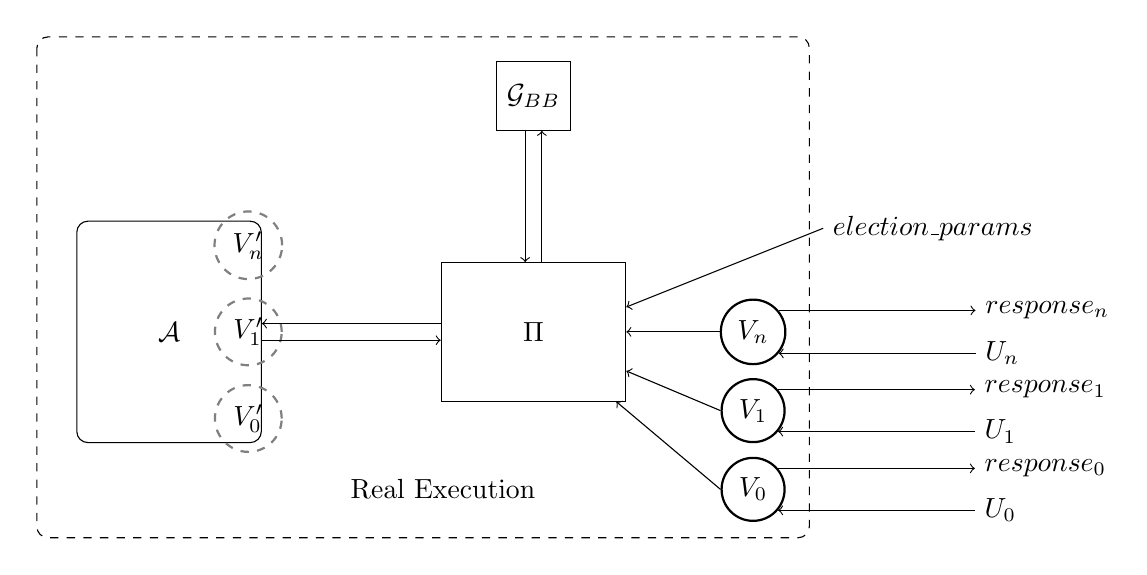
\begin{tikzpicture}
    \node (s) [a] {$\mathcal{A}$};
    \path (s.east)+(1.5*\blockdist,3) node (g) [sensor] {$\mathcal{G}_{BB}$};
    \path (s.east)+(1.5*\blockdist,0) node (system) [s] {$\Pi$};
    \path (system.east) +(0.7*\blockdist,-2) node (v0) [v] {$V_0$};
    \path (system.east) +(0.7*\blockdist,-1) node (v1) [v] {$V_1$};
     \path (system.east) +(0.7*\blockdist, 0) node (vn) [v] {$V_n$};
     \path (s.west) +(0.95*\blockdist,-1.1) node (v0') [vv] {$V_0'$};
      \path (s.west) +(0.95*\blockdist,0) node (v1') [vv] {$V_1'$};
       \path (s.west) +(0.95*\blockdist,1.1) node (vn') [vv] {$V_n'$};
    \path (s.east) +(\blockdist, -2) node (RE) {Real Execution};
    \draw[transform canvas={yshift=0.7ex},->] (system) -- (s);
    \draw[transform canvas={yshift=-0.7ex},<-] (system) -- (s);
    \draw[transform canvas={xshift=0.7ex},->] (system) -- (g);
    \draw[transform canvas={xshift=-0.7ex},<-] (system) -- (g);
     \path [draw, <-] (system) --  (v1.west);
      \path [draw, <-] (system) -- (v0.west);
      \path [draw, <-] (system) --  (vn.west);
    \draw [<-] (v0.-40)-- node [ann] {} + (\edgedist,0) 
        node[right] {$U_0$};
      \draw [<-] (v1.-40)-- node [ann] {} + (\edgedist,0) 
        node[right] {$U_1$};
     \draw [<-] (vn.-40)-- node [ann] {} + (\edgedist,0) 
        node[right] {$U_n$};
     \draw [->] (v0.40)-- node [ann] {} + (\edgedist,0) 
        node[right] {$response_0$};
      \draw [->] (v1.40)-- node [ann] {} + (\edgedist,0) 
        node[right] {$response_1$};
     \draw [->] (vn.40)-- node [ann] {} + (\edgedist,0) 
        node[right] {$response_n$};
        \draw [<-] (system.15) -- node [ann] {} + (\edgedist,1) 
        node[right] {$election\_params$};
    \begin{pgfonlayer}{background}
        \path (s.west |- g.north)+(-0.5,0.3) node (a) {};
        \path (v0.south -| v0.east)+(+0.3,-0.2) node (b) {};
        \path[rounded corners, draw=black, dashed]
            (a) rectangle (b);
    \end{pgfonlayer}
\end{tikzpicture}
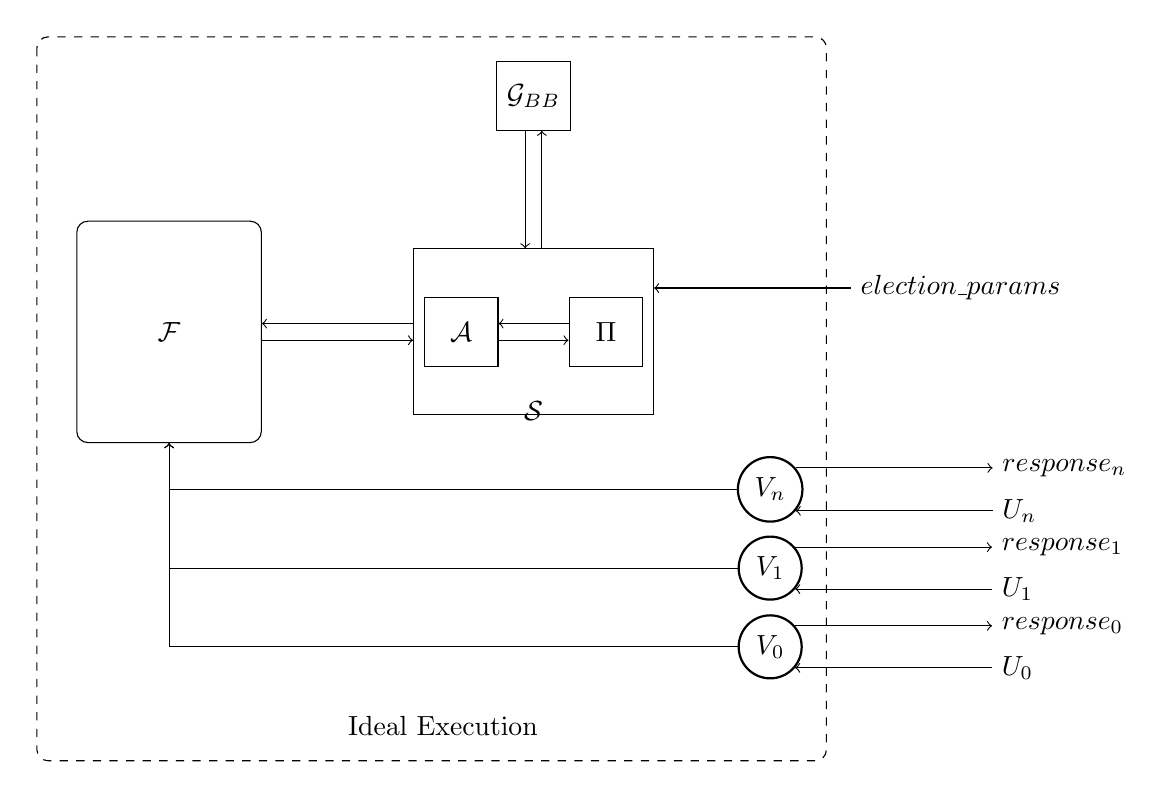
\begin{tikzpicture}
    \node (s) [a] {$\mathcal{F}$};
    \path (s.east)+(1.5*\blockdist,3) node (g) [sensor] {$\mathcal{G}_{BB}$};
    \path (s.east)+(1.5*\blockdist,0) node (system) [sim] {};
    \path (s.east)+(1.1*\blockdist,0) node (adv) [sensor] {$\mathcal{A}$};
     \path (s.east)+(1.9*\blockdist,0) node (ss) [sensor] {$\Pi$};
    \path (ss.east) +(0.7*\blockdist,-4) node (v0) [v] {$V_0$};
    \path (ss.east) +(0.7*\blockdist,-3) node (v1) [v] {$V_1$};
     \path (ss.east) +(0.7*\blockdist, -2) node (vn) [v] {$V_n$};
    \path (s.east) +(\blockdist, -5) node (RE) {Ideal Execution};
     \path (s.east) +(1.5*\blockdist, -1) node (ssimulator) {$\mathcal{S}$};
    \draw[transform canvas={yshift=0.7ex},->] (system) -- (s);
    \draw[transform canvas={yshift=-0.7ex},<-] (system) -- (s);
    \draw[transform canvas={xshift=0.7ex},->] (system) -- (g);
    \draw[transform canvas={xshift=-0.7ex},<-] (system) -- (g);
    \draw[transform canvas={yshift=0.7ex},->] (ss) -- (adv);
    \draw[transform canvas={yshift=-0.7ex},<-] (ss) -- (adv);
     \path [draw, <-] (s) |-  (v1.west);
      \path [draw, <-] (s) |- (v0.west);
      \path [draw, <-] (s) |-  (vn.west);
    \draw [<-] (v0.-40)-- node [ann] {} + (\edgedist,0) 
        node[right] {$U_0$};
      \draw [<-] (v1.-40)-- node [ann] {} + (\edgedist,0) 
        node[right] {$U_1$};
     \draw [<-] (vn.-40)-- node [ann] {} + (\edgedist,0) 
        node[right] {$U_n$};
     \draw [->] (v0.40)-- node [ann] {} + (\edgedist,0) 
        node[right] {$response_0$};
      \draw [->] (v1.40)-- node [ann] {} + (\edgedist,0) 
        node[right] {$response_1$};
     \draw [->] (vn.40)-- node [ann] {} + (\edgedist,0) 
        node[right] {$response_n$};
        \draw [<-] (system.20)-- node [ann] {} + (\edgedist,0) 
        node[right] {$election\_params$};
    \begin{pgfonlayer}{background}
        \path (s.west |- g.north)+(-0.5,0.3) node (a) {};
        \path (RE.south -| v0.east)+(+0.3,-0.2) node (b) {};
        \path[rounded corners, draw=black, dashed]
            (a) rectangle (b);
    \end{pgfonlayer}
\end{tikzpicture}
        \caption{Real and Ideal Execution}
        \label{ RI}
\end{figure}\\
Security requires the existence of some simulator program $\mathcal{S}$ such that the real and ideal executions are indistinguishable for and any environment  $\mathcal{Z}$. Unfortunately, as we are about to show, no such simulator exists.
\begin{theorem} 
For any system $\Pi$ that satisfies the definition of strict privacy, there is an adversary $\mathcal{A}$  such that for any simulator $\mathcal{S}$, there is an environment $\mathcal{Z}$ that distinguishes ideal and real executions $\exec_{\mathcal{Z}, \mathcal{S}}^{\mathcal{F}, \mathcal{G}_{BB}} \not \approx \exec_{\mathcal{Z},\mathcal{A}}^{\Pi, \mathcal{G}_{BB}}$ 
\end{theorem}

\section{Proof part 1: E2E Verifiability vs Strict privacy with respect to $\ea$ and $\T$.}
Suppose there is a system $\Pi$, which is strictly private in case ``$\ea$ is corrupted, but $\vsd$ and $\T$ are honest".\\
Consider the following attack against E2E Verifiability: \\
\fbox{\begin{minipage}{30em}
$\mathcal{A}$:\\
-- corrupts $\ea$ and $\vsd$s but doesn't corrupt $\asd$s.\\
-- corrupts $t$ voters $(t \leq n)$ , where $n$ is the total number of voters.\\ 
-- creates fake voters $\{V_0',V_1',\dots,V_n'\}$ and using its power substitutes some part $\gamma$ of honest voters with fake ones for the $U_a$ option.\\
-- fake voters vote for adversarial options according to a vote-casting procedure.\\
-- substituted honest voters receive receipts generated for fake voters.
\end{minipage}}\\\\
  \begin{figure}[h!]
 \includestandalone[mode=buildnew]{figures/attack}
        \caption{  $\mathcal{A}$}
\end{figure}\\
let $\mathcal{Z}$ be the environment that works as follows:\\\\
\fbox{\begin{minipage}{30em}
$\mathcal{Z}$:\\
--  defines an election setup information:\\ $election\_params = (\mathcal{C},\mathcal{V}, \mathcal{U}, params)$, where $\mathcal{C}$ - list of candidates, $\mathcal{V}$ - list of voters, $\mathcal{U}$ - list of allowed candidates' selections, $params$ - other required information.\\
-- instructs each voter $V_i$ to vote for the blank $'no~one'$ option.\\
-- stops the vote-casting phase.\\
-- asks $\mathcal{G}_{BB}$ for the election result $\tau$\\
--  asks every voter $V_i$ to verify his choice and return the result of verification - $response_i$, where $response_i$ equal to $(sid, verify\_responce, \tau')$  in case of successful verification and $\bot$ otherwise.\\
-- If the number of successful verification responses equal to the number of voters and in all responses provided by a voter tally $\tau'$ is equal to the $\mathcal{G}_{BB}$'s tally $\tau$ return 1. Otherwise return 0.
\end{minipage}}
\\\\
 Since $\Pi$ is strictly private, probability, that an adversary $\mathcal{D}$ engaging in the \textbf{Cast} protocol would distinguish real and simulated view and win the attack against the strict privacy $Pr[G_{strict,\vsd,\T}^{\mathcal{D},Sim}(1^{\lambda,n,m}) = 1] = \frac{1}{2} + \alpha$ where $\alpha$ is negligible. In case of corrupted $\ea$, $\mathcal{C}$ returns a real pair of ballot and receipt and a real view and also a simulated via $Sim$ pair and fake view. This means that in a strictly private system an adversary has a negligible chance to distinguish the ballot and receipt for his option and for some $U_a$ option. \\\\
During the Real Execution a voter can either accept or reject the cast ballot. Rejection is possible only if he detects that the returned receipt, ballot and view are faked. The probability that a voter distinguish the receipt and ballot for his option from for the `no-one' option and rejects is $\Pr[V_i~rejects] \leq  \alpha$, where $\alpha$ is negligible.\\\\
 By nature of the attack,  fake receipt is the perfectly valid receipt for the $U_a$ option and the cast ballot would always be successfully verified. Therefore in the Real Execution $\mathcal{Z}$ would get a successful verification response from all n voters and output 1 with the probability $\Pr[\exec_{\mathcal{Z},\mathcal{A}}^{\Pi, \mathcal{G}_{BB}} = 1] =  \Pr[all~V_i~accept] = \prod_{i=0}^n(1- \Pr[V_i~rejects] ) \geq (1 - \alpha)^n = 1 - n\alpha = 1- \beta$, where $\beta = n\alpha $ is negligible. Thus, $\Pr[\exec_{\mathcal{Z},\mathcal{A}}^{\Pi, \mathcal{G}_{BB}} = 0] = 1 - \Pr[\exec_{\mathcal{Z},\mathcal{A}}^{\Pi, \mathcal{G}_{BB}} = 1] \leq \beta$, where $\beta$ is negligible.\\\\
Suppose for the sake of contradiction that $\Pr[\exec_{\mathcal{Z},\mathcal{A}}^{\Pi, \mathcal{G}_{BB}} = 0] \geq  \beta$, where $\beta$ is non-negligible. This means that at least one voter rejects the receipt. We will show that this contradicts the definition of strict privacy. Consider an attacker $\mathcal{B}$ against strict privacy which exploits the environment  $\mathcal{Z}$. \\\\
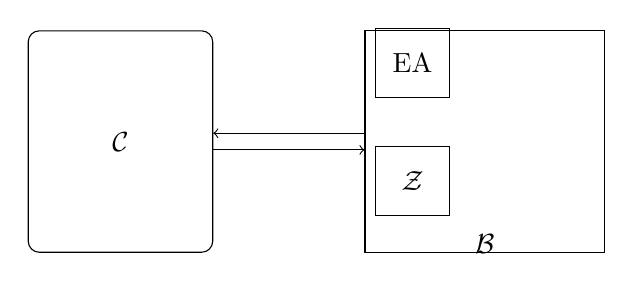
\begin{tikzpicture}
    \node (s) [a] {$\mathcal{C}$};
    \path (s.east)+(1.5*\blockdist,0) node (system) [draw, text width=8em, 
    text centered, minimum height=8em] {};
    \path (s.east)+(1.1*\blockdist,1) node (adv) [sensor] {$\ea$};
     \path (s.east)+(1.1*\blockdist,-0.5) node (ss) [sensor] {$\mathcal{Z}$};
     \path (s.east) +(1.5*\blockdist, -1.3) node (ssimulator) {$\mathcal{B}$};
    \draw[transform canvas={yshift=0.7ex},->] (system) -- (s);
    \draw[transform canvas={yshift=-0.7ex},<-] (system) -- (s);
\end{tikzpicture}

\fbox{\begin{minipage}{30em}
$\mathcal{B}$ interacts with the challenger in the strict privacy attack  $\mathcal{C}$ as follows: \\
-- $\mathcal{Z}$ defines an election parameters  $election\_params$, assign every voter to vote for the blank option $\{V_i,`no~one'\}$ and send this information to the $\mathcal{B}$.\\
-- $\mathcal{B}$ forwards received $election\_params$ to the $\ea$. \\
-- $\mathcal{B}$ corrupts the $\ea$.\\
-- $\ea$ starts the election.\\
-- $\mathcal{B}$ interacts with the challenger $\mathcal{C}$ provides  $(V_i,`no~one',U_{\mathcal{Z}_i})$ as the input.\\ 
--  $\mathcal{C}$ sends back to the $\mathcal{B}$ real and simulated view $(b_0,r_0), (b_1,r_1)$ in the order defined by the challenger's coin a. \\
-- $\mathcal{B}$ votes on behalf of all voters\\
-- $\mathcal{Z}$ stops the vote-casting phase.\\
--  $B$ computes the election's tally and proof of the tally's correctness.\\
-- $\mathcal{Z}$ asks $\mathcal{G}_{BB}$ for the election result $\tau$\\
-- $\mathcal{Z}$ requests every voter to verify his ballot correctness.\\
-- $\mathcal{B}$ will run the verification on behalf of all voters using ballots and receipts from $\{b_0,r_0\}$.\\
-- $\mathcal{Z}$ outputs 1 or 0 depending on the voters' verdict.\\
--$\mathcal{B}$ outputs whatever the $\mathcal{Z}$ outputs.
\end{minipage}}\\\\
The challenger $\mathcal{C}$  outputs simulated ballot and receipt as $(b_0,r_0)$, when the coin $a=0$ and as $(b_1,r_1)$ otherwise.\\\\
In case when $a=0, \mathcal{B}$'s behaviour is identical to the $\mathcal{A}$'s strategy and $\mathcal{B}$ wins if $\mathcal{Z}$ outputs 0, which happens if at least one voter rejects the simulated receipt.  By assumption $\Pr[\exec_{\mathcal{Z},\mathcal{A}}^{\Pi, \mathcal{G}_{BB}} = 0] \geq  \beta$, where $\beta$ is non-negligible. Therefore if $(b_0,r_0)$ is the set of simulated ballot and receipt, $\mathcal{B}$ wins with the probability $Pr[\mathcal{B} \rightarrow 0| a=0] = \Pr[\exec_{\mathcal{Z},\mathcal{A}}^{\Pi, \mathcal{G}_{BB}}~=~0] \geq \beta$, where $\beta$ is non-negligible. \\\\
On the other hand, when $a=1$, $\mathcal{B}$ plays honestly and the probability of $\mathcal{Z}$ outputting 1 is equal to probability that all voters successfully verify their votes in the honest execution, which is happens with overwhelming probability $1-negl(\lambda)$.\\\\ 
The probability of $\mathcal{B}$  winning the attack against the strict privacy is \\$\Pr[G_{strict}^{\mathcal{B}}(1^{\lambda})=1]= \Pr[\mathcal{B} \rightarrow 0| a=0]\Pr[a=0] + \Pr[\mathcal{B} \rightarrow 1| a=1]\Pr[a=1] =  \Pr[\exec_{\mathcal{Z},\mathcal{A}}^{\Pi, \mathcal{G}_{BB}}=0]\Pr[a=0]  + \Pr[\exec_{\mathcal{Z},honest}^{\Pi, \mathcal{G}_{BB}} =1]\Pr[a=1] \geq \frac{1}{2}\beta+ \frac{1}{2} - negl(\lambda)$ , where $\beta$ is not negligible. This implies that $\mathcal{B}$ wins the attack against strict privacy with the probability more than $\frac{1}{2} + negl(\lambda)$, which contradicts the assumption that the $\Pi$ is strictly private.\\\\
In the Ideal Execution any simulator $S$ can either:\\
1) post in $\mathcal{G}_{BB}$ the tally $\tau'$ generated by $\mathcal{A}$ or any other tally  $\tau' \neq \tau$\\ 
or\\
2) ignore the $\mathcal{A}$'s tally and post the actual tally $\tau$.\\\\
In the first case, the ideal functionality for E2E verifiability  $\mathcal{F}$  would always detect the tally deviation caused by $\mathcal{A}$ if such exists. And since  $\mathcal{A}$ doesn't corrupt $\asd$s, for all honest voters the ideal functionality $\mathcal{F}$ would block verification responses. This implies that in the Ideal Execution $\exec_{\mathcal{Z}, \mathcal{S}}^{\mathcal{F}, \mathcal{G}_{BB}}$ $\mathcal{Z}$ would get no response from honest voters. The total number of successful verifications would be equal to the number of corrupted voters, which is less (if not voters are corrupted) than the total number of voters -- $\mathcal{Z}$ outputs 0.  \\\\
In the second case, there exists a class of simulators which ignore $\mathcal{A'}$ actions and post the actual tally.  For those simulators consider an modified  environment $\tilde{\mathcal{Z}}$ that works as follows:\\\\
\fbox{\begin{minipage}{33em}
$\tilde{\mathcal{Z}}$:\\
Outputs a bit according to the following rules:\\
$ \begin{cases}
 \text{if} ~~\mathcal{Z}~~ \text{outputs 1 and the number of non-blank votes greater or equal}~~ \gamma \text{-- output 1} \\ 
 \text{else output 0}
\end{cases}$
\end{minipage}}

$\tilde{\mathcal{Z}}$ would still output 1 in case of the real execution since the number of non-blank votes would be at least $\gamma$ due to successful attack  $\mathcal{A}$. However  $\tilde{\mathcal{Z}}$ would not find at least $\gamma$ non-blank votes and output 0 in the ideal execution. \\\\
Thus, there is the attacker $\mathcal{A}$ such that for any simulator $\mathcal{S}$ there is the environment $\tilde{\mathcal{Z}}$ or $\mathcal{Z}$ which can always distinguish real and ideal executions. \\

\section{Proof part 2: E2E Verifiability vs Strict privacy with respect to $\vsd$ and $\T$.}
Suppose there is a system $\Pi'$, which is strictly private in case ``$\ea$ is honest, but $\vsd$ is corrupted".\\
Consider the following attack against E2E Verifiability: \\
\fbox{\begin{minipage}{30em}
$\mathcal{A'}$:\\
-- corrupts $\ea$ and $\vsd$s but doesn't corrupt $\asd$s.\\
-- chooses an option $U_a \in \mathcal{U}$\\
-- corrupts $t$ voters $(t \leq n)$ , where $n$ is the total number of voters.\\ 
-- provides every honest voter $V_i$ with fake credentials $s_i'$ s.t. the ballot and receipt produced using $(s_i',`no~one')$ are identical to the ballot and receipt produced using real credentials for an option $U_a$: $b,r \leftarrow (s_i',`no~one') $ AND $ b,r \leftarrow (s_i,U_a)$\\
-- creates fake voters $\{V_0',V_1',\dots,V_n'\}$ and provides them with real credentials $s_i$\\
--  using its power substitutes some part $\gamma$ of honest voters' cast protocols with the fake voters' protocols for the $U_a$ option.
\end{minipage}}\\\\
let $\mathcal{Z'}$ be the environment that works as follows:\\\\
\fbox{\begin{minipage}{30em}
$\mathcal{Z'}$:\\
--  defines an election setup information:\\ $election\_params = (\mathcal{C},\mathcal{V}, \mathcal{U}, params)$, where $\mathcal{C}$ - list of candidates, $\mathcal{V}$ - list of voters, $\mathcal{U}$ - list of allowed candidates' selections, $params$ - other required information.\\
-- instructs each voter $V_i$ to vote for the blank option (`no~one').\\
-- stops the vote-casting phase.\\
-- asks $\mathcal{G}_{BB}$ for the election result $\tau$\\
--  asks every voter $V_i$ to verify his choice and return the result of verification - $response_i$, where $response_i$ equal to $(sid, verify\_responce, \tau')$  in case of successful verification and $\bot$ otherwise.\\
-- If the number of successful verification responses equal to the number of voters and in all responses provided by a voter tally $\tau'$ is equal to the $\mathcal{G}_{BB}$'s tally $\tau$ return 1. Otherwise return 0.
\end{minipage}}
\\\\
Since $\Pi'$ is strictly private, probability, that an adversary engaging in the \textbf{Registration} protocol would distinguish real and simulated view and win the attack against the strict privacy $|\Pr[G_{strict,\ea}^{\mathcal{A},Sim}(1^{\lambda},n,m) = 1] - \frac{1}{2}| = \alpha$ where $\alpha$ is negligible. In case ``$\ea$ is honest, but $\vsd$ is corrupted'', simulated view is credentials $\tilde{s_i}$ generated via the simulator $Sim$. \\\\
%%%%%
In the Real Execution a voter $V_i$ starts the Cast protocol using fake credentials $s_i'$ and an option $`no~one'$. However, $\mathcal{A'}$ substitutes his ballot and receipt with the ballot and receipt generated for a fake voter with real credentials and $U_a$ option. By nature of the attack, the returned receipt generated for real credentials and the $U_a$ option is identical to the receipt produced for a fake credentials and $`no~one'$ option. Therefore in the Real Execution $\mathcal{Z'}$ would output 1 if non of the voters would detect that he was given a receipt for fake credentials. The probability of this event is $\Pr[\exec_{\mathcal{Z'},\mathcal{A'}}^{\Pi', \mathcal{G}_{BB}} = 1] =  \Pr[all~V_i~accept] = \prod_{i=0}^n(1- \Pr[V_i~rejects] )$. Suppose, the probability of rejection by $V_i$ is $ \Pr[V_i~rejects] = \zeta$. Thus,   $\Pr[\exec_{\mathcal{Z'},\mathcal{A'}}^{\Pi', \mathcal{G}_{BB}} = 1] = (1 - \zeta)^n = 1 - n\zeta = 1- \zeta'$.\\\\
%%%%
Suppose that $ \zeta'$ is not negligible. This means that $\Pr[\exec_{\mathcal{Z'},\mathcal{A'}}^{\Pi', \mathcal{G}_{BB}} = 0] = 1 - \Pr[\exec_{\mathcal{Z'},\mathcal{A'}}^{\Pi', \mathcal{G}_{BB}} = 1] =  \zeta'$, where $ \zeta'$ is not negligible. This means that at least one voter rejects the receipt with a non-negligible probability. We will show that this contradicts the definition of strict privacy. Consider an attacker $\mathcal{B'}$ against strict privacy which exploits the environment  $\mathcal{Z'}$. \\\\
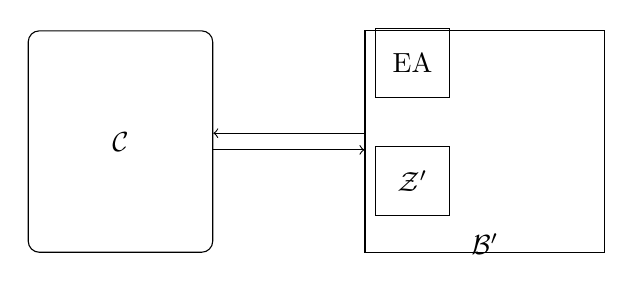
\begin{tikzpicture}
    \node (s) [a] {$\mathcal{C}$};
    \path (s.east)+(1.5*\blockdist,0) node (system) [draw, text width=8em, 
    text centered, minimum height=8em] {};
    \path (s.east)+(1.1*\blockdist,1) node (adv) [sensor] {$\ea$};
     \path (s.east)+(1.1*\blockdist,-0.5) node (ss) [sensor] {$\mathcal{Z'}$};
     \path (s.east) +(1.5*\blockdist, -1.3) node (ssimulator) {$\mathcal{B'}$};
    \draw[transform canvas={yshift=0.7ex},->] (system) -- (s);
    \draw[transform canvas={yshift=-0.7ex},<-] (system) -- (s);
\end{tikzpicture}\\\\
\fbox{\begin{minipage}{30em}
$\mathcal{B'}$ interacts with the challenger in the strict privacy attack  $\mathcal{C}$ as follows: \\
-- $\mathcal{Z}$ defines an election parameters  $election\_params$, assign each voter the blank option $\{V_i,`no~one'\}$ and send this information to the $\mathcal{B}$.\\
-- $\mathcal{B'}$ forwards received $election\_params$ to the $\mathcal{C}$. \\
-- $\mathcal{B'}$ corrupts the $\vsd$.\\
-- $\mathcal{C}$ starts the election.\\
-- $\mathcal{B'}$ sends  to $\mathcal{C}$ $(V_i,`no~one',U_a)$.\\
-- $\mathcal{C}$ sends back $s_0,s_1$. \\
--  $\mathcal{B'}$ provides voters with credentials $s_0$ and uses $(s_0,`no~one')$ to produce the ballot and receipt and posts the result on $\bb$.\\ 
-- $\mathcal{Z'}$ stops the vote-casting phase.\\
--  $\mathcal{C}$ executes the $Tally$ protocol.\\
-- $\mathcal{Z'}$ asks $\mathcal{G}_{BB}$ for the election result $\tau$\\
-- $\mathcal{Z'}$ requests every voter to verify his ballot correctness.\\
-- $\mathcal{B'}$ will run the verification on behalf of all voters.\\
-- $\mathcal{Z'}$ outputs 1 or 0 depending on the voters' verdict.\\
-- $\mathcal{B'}$ outputs whatever the $\mathcal{Z'}$  outputs.\\
\end{minipage}}\\\\
In case when the simulated credentials are chosen ($a=0$), $\mathcal{B'}$ provides a voter with fake credentials and generated ballot and receipt for the blank option using the fake credentials, which means that real credentials correspond to the $U_a$ option. $\mathcal{B'}$'s behaviour is identical to the $\mathcal{A'}$'s strategy. $\mathcal{B'}$ wins if outputs 0, which happens if  $\mathcal{Z'}$ outputs 0. $\Pr[\mathcal{B}'\rightarrow 0| a=0 ] = \Pr[\exec_{\mathcal{Z'},\mathcal{A'}}^{\Pi', \mathcal{G}_{BB}}=0] = \zeta'$\\\\
%
Else if $a=1$, $\mathcal{B'}$ provides a voter with real credentials and uses the real credentials to vote for the blank option, which is honest behaviour. $\Pr[B'\rightarrow 1| a=1] =\Pr[\exec_{\mathcal{Z'},honest}^{\Pi', \mathcal{G}_{BB}}=1] = 1$\\\\
%
Thus, the probability of $\mathcal{B'}$  winning the attack against the strict privacy is \\$\Pr[G_{strict,\ea}^{\mathcal{B}, Sim}(1^{\lambda})=1]= \frac{1}{2}(\Pr[B'\rightarrow 0| a=0] + \Pr[B'\rightarrow 1| a=1])  = \frac{1}{2} (\zeta' +1) =  \frac{1}{2}  +  \frac{1}{2} \zeta'$ , where $\zeta'$ is not negligible. This implies that $\mathcal{B'}$ wins the attack against strict privacy with the probability more than $\frac{1}{2} + negl(\lambda)$, which contradicts the assumption that the $\Pi$ is strictly private.\\\\
In the Ideal Execution any simulator $S$ can either:\\
1) post in $\mathcal{G}_{BB}$ the tally $\tau'$ generated by $\mathcal{A'}$ or any other tally  $\tau' \neq \tau$\\ 
or\\
2) ignore the $\mathcal{A'}$'s tally and post the actual tally $\tau$.\\\\
In the first case, the ideal functionality for E2E verifiability  $\mathcal{F}$  would always detect the tally deviation caused by $\mathcal{A'}$ if such exists. And since  $\mathcal{A'}$ doesn't corrupt $\asd$s, for all honest voters the ideal functionality $\mathcal{F}$ would block verification responses. This implies that in the Ideal Execution $\exec_{\mathcal{Z'}, \mathcal{S}}^{\mathcal{F}, \mathcal{G}_{BB}}$ $\mathcal{Z'}$ would get no response from honest voters. The total number of successful verifications would be equal to the number of corrupted voters, which is less (if not voters are corrupted) than the total number of voters -- $\mathcal{Z'}$ outputs 0.  \\\\
In the second case, there exists a class of simulators which ignore $\mathcal{A'}$ actions and post the actual tally.  For those simulators consider an modified  environment $\tilde{\mathcal{Z'}}$ that works as follows:\\
\fbox{\begin{minipage}{33em}
$\tilde{\mathcal{Z'}}$:\\
Outputs a bit according to the following rules:\\
$ \begin{cases}
 \text{if} ~~\mathcal{Z}~~ \text{outputs 1 and the number of non-blank votes greater or equal}~~ \gamma \text{-- output 1} \\ 
 \text{else output 0}
\end{cases}$
\end{minipage}}

$\tilde{\mathcal{Z'}}$ would still output 1 in case of the real execution since the number of non-blank votes would be at least $\gamma$ due to successful attack  $\mathcal{A}$. However  $\tilde{\mathcal{Z'}}$ would not find at least $\gamma$ non-blank votes and output 0 in the ideal execution. \\\\
Thus, there is the attacker $\mathcal{A'}$ such that for any simulator $\mathcal{S}$ there is the environment $\tilde{\mathcal{Z'}}$ or $\mathcal{Z'}$ which can always distinguish real and ideal executions. 
%% This is an example first chapter.  You should put chapter/appendix that you
%% write into a separate file, and add a line \include{yourfilename} to
%% main.tex, where `yourfilename.tex' is the name of the chapter/appendix file.
%% You can process specific files by typing their names in at the 
%% \files=
%% prompt when you run the file main.tex through LaTeX.
\chapter{Blind signature e-voting scheme}
The idea of obtaining a proof of membership and voting anonymously is not new and had been considered the best possible solution for providing privacy to voters. However most approaches that based on group signatures \cite{Teranishi2009},\cite{Au2013} are traceable because it requires an additional tag that revivals the user's identity in case of exceeding the allowed number of cast votes.\\

A blind signature, on the other hand, makes it absolutely impossible to link a particular voter and his ballot based on published after or during an election information or leakage of authentication data.  It is on of the most popular techniques in e-voting schemes for ensuring confidentiality of the voter's ballot. Blind signatures have been used in many e-voting schemes designed last decades \cite{Ion2011},\cite{Ibrahim2003},\cite{Fujioka1993}. The main feature of the blind signature concept is that it allows to combine two contradictory ideas 1) the authorization of voters and 2)the anonymity of them. It allows to achieve such level of privacy that no one including $\ea$ and $\T$ can link the voter and his ballot. \\

We present an e-voting scheme that is based on the blind signature scheme and the ElGamal encryption, that is Voter Private with respect to trusted $\ea$ and $\T$ but not E2E Verifiable in the standard model. We argue that any e-voting scheme that keeps anonymous ballots is not E2E verifiable in the standard model.
\section{Presentation of the blind signature e-voting scheme}
Our system is a two-server web-based system. The first server - \textit{Signing server}  is used for \textbf{Registration} process and the second one  - \textit{$\voc$} for vote-casting. During the election process, the \textit{Signing server} plays the roles of the $\ea$. Trustee $\T$ is a separate entity that has a secure channel to communicate with $\ea$, security of communication is supported by HTTPS. $\vsd$s are realised by Javascript running at the client side. The system uses additive ElGamal encryption, so the tally is done homomorphically. Currently, the blind signature  scheme supports approval type of voting s.t. $x$-out-of-$m$ type of option selection, where x is between 0 and $m$.
\section{Setup and parameters}
Throughout the paper, it is assumed that a group of $n$ voters $\mathcal{V} = \{V_1,\dots,V_n\}$ can choose as many candidates as they like among the set of $m$ candidates $\mathcal{P} = \{P_1,\dots,P_m\}$, $n$ and $m$ are both thought as polynomial functions of security parameter $\lambda$. Also, during the vote casting procedure no 'write-in's votes are allowed, the number of candidates $m$ is fixed. A voter may cast any vote including a blank or an invalid votes. \\

We denote by $M$ a strict upper bound on the number of votes any candidate can receive. In case when each voter has only one vote, M is a strict upper bound on the number of voters $n$.\\ 

It is assumed that the message space is $\mathbb{Z}_n$ for a suitable $n > M^m$, the $l_R$-bit randomizer size is  $\mathbb{Z}$. For NIZK proofs the cryptographic hash-function that outputs an $l_e$-bit number $e$ is used. In case of SHA-256  $l_e$ = 256. A security parameter $l_s$ is such that for any value $a$, its sum with a random $|a| + l_s$-bit number $a + r_a$ and this random number $r_a$ are indistinguishable. Article \cite{Groth2005} suggests to use $l_s = 80$, since this value is large enough to ignore the off chance that $|a+r| > |a|+l_s$.

\section{Syntax}
An e-voting system $\Pi$ is a tuple of algorithms and protocols $\langle$ \textbf{Setup,Register, Cast,Tally, Result,Verify} $\rangle$ specified as follows:
\begin{enumerate}
\item \textbf{Setup}: The algorithm \textbf{Setup($1^{\lambda}, \mathcal{P}, \mathcal{V}, \mathcal{U}$)}  is executed by the $\ea$ and $\T$. During the setup phase $\ea$ generates $\Pi$'s public parameters $PubEA$ (which include $P, V, U$, $pkey, snPkey, params$), where $params$ are public election data, $pkey$ is the public key for encrypting votes and $snPkey$ is the public key that is used during the registration process for obtaining a blind signature. $\ea$ posts  $PubEA$  the on $\bb$ . Also, $\ea$ the voters' secrets $s_1, \dots , s_n$, that includes a unique salt seed $seed_i$ for AES encryption, a voter's login $login_i$ and password $password_i$ that are used for signing in. $\ea$ distributes secrets among all voters. At the same time, $\T$  obtains secret keys $skey$ and $snSkey$ for decrypting ballots and signing respectively and generates pre-election $\bb$ data $PubT$ and posts it on $\bb$. The public data is defined as $Pub = \langle PubEA, PubT \rangle $. 
\item  \textbf{Register}: The algorithm \textbf{Register($login_i,password_i,id_i$)}  is executed by each voter. A voter $V_i$ randomly chooses a $l_b$-bit string $x_i$ as his alias and a blinding factor $z_i$. He uses $x_i$, $z_i$ and $snPkey$ to construct the value $p_i = Hash(x_i)Enc(z_i;snPkey)$. The voter sends value $p_i$ to the $\ea$ along with his $login_i$, $password_i$ and proofs of identity $id_i$.
\item  \textbf{Cast}:  The interactive protocol \textbf{Cast($vote_i,x_i$)} is executed between tree parties, the voter $V_l$, the $\bb$and the $\voc$. During this interaction, the voter uses $\vsd$ to cast an encrypted ballot $b_i = \langle C, \alpha_i, \pi_i, hash_i, \rangle$, where $C=Enc(vote_i;r)$, $hash_i$ - HASH of entire ballot,  $\alpha_i$ and $\pi_i$  are non-interactive zero-knowledge proofs of eligibility and vote correctness respectively. Upon successful termination, $\voc$ posts ballot $b_i$ to $\bb$. The voter $V_l$ receives nothing.
\item  \textbf{Tally}: The interactive protocol \textbf{Tally($Pub$)}  can be executed by anyone due to a homomorphic property of the encryption scheme. The output is an encrypted sum of all valid ballots $\tau$ or $\perp$ in case all entries are invalid.
\item   \textbf{Result}: The algorithm  \textbf{Result($\tau, sKey$)} performs the decryption and outputs the result $R_{\tau}$ of the election and proofs of correct decryption $\pi_{\tau}$ or returns  $\perp$in case such result is undefined.
\item  \textbf{Verify}: The algorithm \textbf{Verify($b_i$)} outputs 1 if ballot $b_i$ is valid and 0 otherwise.
\end{enumerate}

\section{Building blocks}
\subsection{Blind signature}
In cryptography digital signature allows to 'sign' massage so everyone can verify the validity of the signature, but no one can  produce a \textit{new} signature for some new message. One variation of digital signatures is the blind signature scheme, that is the basic signature with the additional requirement that a signer should 'sign' messages without knowing its content. The concept of blind signing was introduced by David Chaum in \cite{Chaum1982}. \\

The global idea is to form a specially constructed message that hides a secret, obtain a signature for this message and then construct a valid signature for the secret. Suppose Alice wants Bob to sign a value $x$ with his private key $skey = (d,N)$ without learning $x$. To do so, Alice picks random blinding factor $z$ such that  $gcd(z,N) = 1$ and calculates $p=xz^e\bmod N $. She sends value $p$ to Bob. Bob signs $p^d\bmod N$ and sends it back to Alice. Alice calculates $p^d\bmod N z^{-1} = x^d\bmod N$ which is a signature for value $x$. Bob in not able to determine the secret $x$ on his own due to multiplication on unknown blinding factor. Blind signature can not be broken even with a help of a quantum computer.\\\\
\fbox{\begin{minipage}{30em}
\textit{Public input}:   $pkey = (e,N)$\\
\textit{Private input}:   $skey = (d,N)$\\\\
\textbf{Argument to sign:}\\
$p=xz^e\bmod N $\\
\textbf{Constructing signature}:\\
$p^d\bmod N z^{-1} =x^dz z^{-1} \bmod N =  x^d\bmod N$
 \end{minipage}}\\\\
Security of the blind signature scheme relies on an information assumption and does not rely on a computational one, so it achieves information-theoretic security considered to be cryptanalytically unbreakable. That means that even an adversary $\mathcal{A}$ with unlimited computing power can not break the blind signature scheme because  $\mathcal{A}$ simply does not have enough information to break the encryption.\\

Also, Chaum's blind signature satisfies the blindness property \cite{Chaum1982} and the non-forgeability \cite{Pointcheval1996},\cite{Abstract1997} of additional signatures, the former means that a signer can not  link the blinded message he signs and the original one except with negligible probability, and letter means that after getting $l$ signatures, it is infeasible to compute the $l+1$ signature.\\

Informally, unlinkability or blindness can be proven as follows. For any message $m$  there is a unique set of values $r_1,r_2,\dots,r_n$ that produces a set of blinded messages $m'_1,m'_2,\dots,m'_n$, with $mi_i  \equiv mr_i^e$. No set of values $r_1,r_2,\dots,r_n$ is any more probable than any other, hence the signer gets no information whether $m$ corresponds to $m'_1$ or $m'_2$ or whether it was one of the values signed at all.\\

One can implement the blind signature scheme with almost any common public key encryption scheme. For our scheme we use one of the simplest blind signature schemes, that is based on RSA encryption. 
\subsection{Homomorphic Integer Commitment and Homomorphic Cryptosystem}
There are only a few homomorphic integer commitment schemes \cite{Eiichiro1997},\cite{Damg},\cite{Groth2005a} and they are quite similar in structure. For the blind signature scheme  we use the commitment scheme described in  \cite{Groth2010}: "A modulus $n$ as a product of two safe primes and random generators $g_1, \dots, g_k,h$ of $QR_n$ are chosen. In order to commit to integers $m_1,m_2, \dots, m_k$ using randomness $r$, it is necessary to compute $c = com( m_1,m_2, \dots, m_k; r) = g_1^{m_1}g_2^{m_2}\dots g_k^{m_k}h^r$". The commitment is statistically hiding if the randomness choice is $r \leftarrow \{0,1\}^{l_r}$.\\

To prove soundness and knowledge in protocols, we need a root extraction property. This property basically says that "if a ciphertext raised to a nontrivial exponent encrypts 1, then the ciphertext itself encrypts 1" \cite{Groth2010}. For the homomorphic encryption generalisation of this property can be formalized as follows \cite{Groth2005}: \\
\begin{definition}[Root extracting property \cite{Groth2005}]
If there is a ciphertext $C$ and $e \neq  0$ so $|e| < l_e$ and $C^e = E(M;R)$, then it must be possible to find $\mu, \rho$ so $M = e\mu$,$R = e\rho$ and $C = E(\mu; \rho)$. 
\end{definition}

ElGamal encryption scheme  is an asymmetric key encryption algorithm for public-key cryptography with an implementation of Diffie-Hellman key distribution system  that was introduced  by Taher Elgamal in 1985 \cite{Elgamal1985}. The security of the scheme relies on the difficulty of computing the discrete logarithm over finite fields.  ElGamal encryption is semantically secure, has the root extraction property and admit threshold decryption  \cite{Groth2010}. \\

The use of homomorphic tallying scheme for e-voting is not new, it was originally introduced by Cramer et al. \cite{Cramer1997}  in 1997. From the E2E Verifiability point of view, the major benefit of using homomorphic tallying is that the proof of correct tallying and decryption is simplified and can be publicly verified if all encrypted votes are public \cite{Parsovs2016}. This means that tallied as recorder verification can be simplified and re-checked by anyone.  Moreover, the aggregated ciphertext and the corresponding plaintext cannot be linked back to individual votes. Publishing encrypted ballots can leas to long-term privacy risks, for example, the encryption may be broken after a few decades. One may mitigate the risks by limiting the access to $\bb$, where all encrypted ballots are stored. However, for the \textit{Blind signature scheme} we prefer to publish all encrypted ballots to achieve  public verifiability.\\

If tallied as recorder can be checked simply by anyone, then the only  verifiability feature still missing (except for cast as intended check) is to verify that all ballots are correctly formed and contains no more than one vote per candidate. This means that ballots should be submitted along with the zero-knowledge cryptographic proof of correctness. 
\subsection{Proving signature knowledge}
Non interactive zero knowledge (NIZK) proof  of signature knowledge a method by which one party (the prover) can successfully convince another party (the verifier) that the prover knows something without conveying any information apart from that fact.\\

Suppose there is a signature $\sigma$ for a hash value over message $x$ $HASH(x)$. Now a prover want to convince a verifier that he knows the signature without revealing value $\sigma$. The prover chooses a random variable $A$ and encrypt it using the public key $pkey = (e,N)$. Then he computes a product $S$ of the encrypted value and the signature raised in power of a challenge $c$. In the non-interactive proofs the challenge $c$ typically equal to the result of a hash function over the concatenation of all publicly known variables and arguments that is used for proving the statement. The NIZK argument is the challenge $c$ and the product $S$.\\\\
\fbox{\begin{minipage}{30em}
\textbf{Non-Interactive Zero-Knowledge Argument for proving signature knowledge:}\\\\
\textit{skey}:  (d,N)\\
\textit{pkey}:  (e,N)\\\\
Proof of the signature knowledge:\\
$NIZK[(x,\sigma): \sigma = x^d\bmod N]$\\\\
\textbf{Argument:}\\
$\sigma = HASH(x)^d\bmod N$\\
Choose random $A \in _R Z_N$\\
$R = A^e\bmod N$\\
$c = HASH(x||R)$\\
$S = A\sigma^c\bmod N$\\
The argument is: $(c,S)$\\\\
\textbf{Verify:}\\
$\hat{R} = \frac{S^e}{HASH(x)^c}\bmod N$\\
$\hat{c} = HASH(x||\hat{R})$\\
Verify $\hat{c} = c$
\end{minipage}}\\

Indeed if $\hat{c} = HASH(x|| \frac{S^e}{HASH(x)^c}\bmod N )= HASH(x|| A^e\bmod N ) =  HASH(x||R) = c$ then proofs of signature knowledge are valid.
\subsection{Proving that a ciphertext encrypts 0 or 1}
The following NIZK proof was designed by Jens Groth \cite{Groth2005}. \\

Each voter $V_i$ can vote for as many candidates from the set of all candidates as he likes. The voter specifies his choice by setting $a_j = 1$ if he wishes to vote for candidate $j$ and $a_j = 0$ if he does not. The plaintext vote is $VOTE_i =\sum_{j=0}^{m-1}a_jM^j$. The voter encrypts this to get a ciphertext $C = E(\sum_{j=0}^{m-1}a_jM^j;R)$. He now needs to prove that indeed the plaintext is on the right form so $a_j = 0 \vee 1$ for all $j \in [0,m-1]$. \\

A prover commit to values $a_0, \dots , a_{m-1}$. In order to prove that all hidden $a_j \in \{0, 1\}$  the fact that $x^2 \geq x$ for any integer and equality holds only for $x = 0$ or $x = 1$ is used. This means that if the prover want to convince the verifier that  all $a_j$'s belong to $\{0, 1\}$ he needs to convince him that $\Delta = \sum_{j=0}^{m-1}(a_j^2  - a_j) = 0$.\\

The variables $a_j$ and $\Delta$ are hidden using the standard techniques $\boxed{a_j} = ea_j +r_{a_j}$  and $\boxed{\Delta} = e\Delta+r_\Delta$. In the verification, the verifier construct the same value $\boxed{\Delta} = \sum_{j=0}^{m-1}(\boxed{a_j}^2  - e\boxed{a_j})$. The left side of this equation  is a degree 1 polynomial in $e$ while the right side is a degree 2 polynomial in $e$. With overwhelming probability over $e$ this implies that the value the prover committed to $\Delta =0$, which is exactly what needs to be proven.\\
 
 The rest of the NIZK argument are a proof of knowledge of the plaintext $V$ and a proof that this plaintext has been properly constructed with values $a_j$'s that the prover committed to.\\\\
\fbox{\begin{minipage}{30em}
\textbf{Non-Interactive Zero-Knowledge Argument for Correctness of the encrypted vote:}\\\\
The proof of correctness:\\
$NIZK[(v,\rho,a_0,\dots, a_{m-1}): C = Encr(v;\rho) \text{ and   } v = \sum_{j=0}^{m-1}a_jM^j $\\
$\text{ and } \sum_{j=0}^{m-1}(a_j^2 - a_j) = 0]$\\\\
\textbf{Argument:}\\
Choose $r_{a_0},\dots r_{a_{m-1}} \leftarrow \{0,1\}^{1+l_s+l_e}$ and let $\Delta = \sum_{j=0}^{m-1}(2a_j -1)r_{a_j}$ \\
Choose $r \leftarrow \{0,1\}^{l_r}$ and set $c = com(a_0,\dots,a_{m-1},\delta;r)$\\
Choose $r_r \leftarrow \{0,1\}^{l_r+l_s + l_e}$ and set $c_r  = com(r_{a_0},\dots,r_{a_{m-1}},\sum_{j=0}^{m-1}r_{a_j}^2;r_r)$\\
$R_v = \sum{j=0}^{m-1}r_{a_j}M^j$, choose $R_R \leftarrow \{0,1\}^{l_R +l_e+l_s}$ and set $C_R = Encr(R_V;R_R)$\\
Compute a challenge $e \leftarrow hash(C,C_R,c,c_r)$\\
Set $\boxed{R} = eR + R_R$. Set $\boxed{a_j} = ea_j + r_{a_j}$ and $\boxed{r} = er + r_r$\\
The argument is: $C_R,c,c_r, \boxed{R},\boxed{a_0},\dots,\boxed{a_{m-1}},\boxed{r}$\\\\
 \textbf{Verification:}\\
 Compute $e$ as above.\\
 Define $\boxed{V} = \sum_{j=0}^{m-1}\boxed{a_j}M^j$ and \\
 $\boxed{\Delta} = \sum_{j=0}^{m-1}(\boxed{a_j}^2 - e\boxed{a_j}).$\\
 Verify $C^eC_R = Encr(\boxed{V};\boxed{R})$ and $c^ec_r = com(\boxed{a_0},\dots,\boxed{a_{m-1}},\boxed{\Delta};\boxed{r})$ 
\end{minipage}}\\

The complete prove of completeness, zero-knowledge as well as soundness and knowledge of the  described NIZK argument  can be found here \cite{Groth2005}.
\section{System Design}
Here is the description of a blind signature e-voting system for r-out-of-m elections, where $0\leq r\leq m$.\\
The Blind signature scheme:\\ 
\textbf{Setup ($1^{\lambda}, \mathcal{P}, \mathcal{V}, \mathcal{U}$).}\\\\
Let ($GenBL, EncrB, SignBL)$ be the PPT algorithms that constitutive the RSA blind signature scheme,  $PRG_{str}$  - a function for pseudo random string generation, $PRG_{prime}$  - a function for pseudo-random prime number generation and $(Gen, Encr, Decr)$ - PPT algorithms for the ELGamal encryption scheme. The EA runs $GenBL(Param, 1^{\lambda})$ to generate the blind signature scheme keys $(bsk, bpk)$ and $Gen(Param, 1^{\lambda})$ to generate ELGamal keys $(sk,pk)$. Public keys $bpk,pk$ and functions $EncrB,Encr, PRG_{str}, PRG_{prime}$ are posted on the BB.\\
Then, for every voter $V_l$, where $l \in [n]$, EA runs $PRG_{str}(1^{\lambda})$ function to generate random string $seed_l$.\\\\
\textbf{Registration}\\\\
Let $(GenAES, EncrAES, DecrAES)$ be the publicly known PPT algorithms that implements AES encryption scheme and $Hash$ - hash algorithm.  \\\\
Every voter $V_l$ completes the following procedure: \\
--  uses the published on the BB function $PRG_{str}(1^{\lambda})$ to generate his alias $x_l$ and  $PRG_{prime}(bpk)$ to generate a blinding factor $z_l$. \\
-- calculates value $p_l = Hash(x_l)EncrB(z_l)$.\\
--  chooses his secret password $password_l$ and runs  $ GenAES(password_l, s_l)$ to generate his key for symmetric encryption $key_l$, where $s_l = PRG_{str}(seed_l)$.\\
--  encrypts $x_l$ and $z_l$ by running  $EncrAES(key_l,x_l)$ and $EncrAES(key_l,z_l)$ respectively to get encrypted values $\hat{x_l},\hat{z_l}$\\
-- sends $p_l,\hat{x_l},\hat{z_l}$ to the EA\\\\
 EA:\\
Upon receiving $p_l,\hat{x_l},\hat{z_l}$ from a voter, EA posts all information to the BB.\\
When registration is closed, EA runs  $SignBL(bsk, p_l)$ for every entry in the BB and post the result in the corresponding line as $p^{sign}_l$.\\\\
\textbf{Cast:}\\
Let $e_l = (e_{1_l},e_{2_l},\dots,e_{m_l})$ be the characteristic vector corresponding to the voter's selection, where $e_{j_l}=1$ if the option $opt_j$ is selected by the voter $V_l$.\\ 
Every voter $V_l$ completes the following procedure:\\
-- gets all information from the BB - $\{p_l,\hat{x_l},\hat{z_l}\}$.\\
-- finds his entry and decrypts $x_l$ and $z_l$ by running $DecrAES(key_l,\hat{x_l})$ and $DecrAES(key_l,\hat{z_l})$ respectively, where $key_l =  GenAES(password_l, s_l)$ and  $s_l = PRG_{str}(seed_l)$\\
-- computes  $\sigma_l$ - signature for $x_l$  by calculating  $p^{signed}_lz_l^{-1}$\\
-- computes $\Pi_l$ -- NIZK proof of signature knowledge .\\
-- chooses his vote-option $e_{j_l}$ and writes the corresponding characteristic vector $e_l$\\
-- for $j \in [m]$ compute $c_{j_l} =  Encr(pk,e_{j_l})$\\
-- computes NIZK proofs $\pi_{j_l}$ that each $c_{j_l}$ is an encryption of 1 or 0.\\
-- sends $b_l = (x_l, \sigma_l, \Pi_l, c_l, \pi_l)$ to the EA.\\
-- keeps $x_l$ as receipt.\\
-- If EA accept $b_l$, protocol terminates successfully.\\ 
*Optional: every voter can export the randomness to check that the ballot was cast as intended.\\\\
Upon receiving $(x_l, \sigma_l, \Pi_l, c_l, \pi_l)$ from a voter, EA checks NIZK proofs and, if it's valid, accepts the ballot and posts all information to the BB.\\\\
\textbf{Tally: }\\
After election is closed, EA computes $\mathcal{C}$ -- the sum of all $c_l$ and runs $Decr(sk, \mathcal{C})$ to decrypt Tally $\tau$. EA posts the $\tau$ along with the proof of tally correctness $Proof$.\\\\
\textbf{Result:} \\
result is straightforward.\\\\
\textbf{Verify:} \\
The algorithm returns 1 only if the following checks are true:\\
--  exported randomness is correct or voter choose not to check.\\
-- there is ballot with $x_l$\\
-- all $\Pi_l, \pi_l$ are valid\\
-- number of ballots less or equal to the number of registered voters\\
-- $Proof$ is correct\\
-- sum of all scores at $\tau$ are less than or equal to ballot numbers\\\\
\section{E2E Verifiability}
In E2E verifiability proofs, we assume that all entities are malicious and controlled by the adversary $\mathcal{A}$ and only $\bb$ is honest, but  $\mathcal{A}$ can arbitrarily change the content of the $\bb$  before executing the \textbf{Result} protocol. However, we assume that validity of all NIZK proofs on the $\bb$ can be checked by anyone as well as the result of the \textbf{Tally} protocol execution, since $Tally$ is computed homomorphically and this computation doesn't require any secret information. To prove that the blind signature scheme is E2E verifiable, we first construct a vote extractor $\mathcal{E}$:\\
 
$\mathcal{E}$ has input $\tau$ and the set of receipts  $\{x_l\}_{V_l \in \tilde{\mathcal{V}}}$ where $\tilde{\mathcal{V}}$ is the set of the honest voters that voted successfully.  If $Result(\tau) = \perp$ (i.e., the transcript is not meaningful), then $\mathcal{E}$ outputs $\perp$. Otherwise, $\mathcal{E}$ (arbitrarily) arranges the voters in $\mathcal{V} \backslash \tilde{\mathcal{V}}$ and the tags not included in $\{x_l\}_{V_l \in \tilde{\mathcal{V}}}$ as $\langle V_l^{\mathcal{E}} \rangle_{l \in  [n - |\tilde{\mathcal{V}}|]}$ and $\langle tag_l^{\mathcal{E}} \rangle_{l \in  [n - |\tilde{\mathcal{V}}|]}$ respectively. Next, for every $l \in [n - |\tilde{\mathcal{V}}|]$:\\
\begin{enumerate}
\item  $\mathcal{E}$ finds at the BB entry with   $x_l = tag_l^{\mathcal{E}}$ and brute-force the corresponding ELGamal cipher to open the selected candidate $\mathcal{P}_l^{\mathcal{E}}$. If $\mathcal{P}_l^{\mathcal{E}}$ is the valid candidate's selection, then $\mathcal{E}$ sets $\mathcal{U}_l^{\mathcal{E}} = \{\mathcal{P}_l^{\mathcal{E}}\}$. Otherwise it inputs $\perp$.
\end{enumerate}
Finally $\mathcal{E}$ outputs  $\langle \mathcal{U}_l^{\mathcal{E}} \rangle_{V_l \in \mathcal{V} \backslash \tilde{\mathcal{V}}  }$
Finally $\mathcal{E}$ outputs  $\langle \mathcal{U}_l^{\mathcal{E}} \rangle_{V_l \in \mathcal{V} \backslash \tilde{\mathcal{V}}  }$\\

According to the definition of E2E verifiability, an adversary $\mathcal{A}$ wins the game $G^{\mathcal{A} ,\mathcal{E} ,d,\theta}_{\text{e2e-ver}} (1^{\lambda}, n,m,t)$ and breaks E2E verifiability if it allows at least $\theta$ honest voters to cast their votes successfully and achieves tally deviation $d$. \\

All NIZK proofs are perfectly sound and the \textbf{Tally} protocol is completely transparent and can be repeated and checked by anyone. Thus, $\mathcal{A}$ can not misinterpret results or encode more than one vote for a particular candidate. The only possible way for $\mathcal{A}$ to cheat is to somehow modify honest votes' intents. \\

\textbf{Modification attack}: $\mathcal{A}$, who controls the whole system, may attempt to modify a ballot by decrypting it, learning $x$, creating a new signature and voting for another candidate, however since each voter has the hash of the whole his ballot as receipt, malicious $\ea$ would be caught. \\

\textbf{Clash attacks}: This attack is statistically improbable, since $x$ is unknown for $\mathcal{A}$ large string picked at random by a voter. If  $\mathcal{A}$ modifies the pseudo-random generator in a way that a number of voters gets the same not random string, it is easily detectable since  this part is done on the client side and the code is available for audition. \\

However $\ea$ can use abstain voters, who registered but did not cast their votes,  to create additional ballots and cause deviation. It can use $y_{reg} - y_{voted} -1$  additional votes. Abstain voter can not prove anything since he doesn't know whether he is the only one who abstains or not. This attack can be detected only if every registered voter is assigned a specific entry in $\bb$. Unfortunately,  assigning every voter ballot id makes this system linkable.\\

There is a tradeoff: either $\ea$ should be able to link an individual voter with his ballot or $\ea$ can vote on behalf of abstain voters and no-one would detect it as long as number of additional ballots strictly less than the number of abstain voters. This attack applies to any e-voting systems that allows voters to vote anonymously.  

\section{Implementation}
The blind signature scheme system is an open source web-based public auditable e-voting system. The system consists of two main servers: \textit{Signing Server} (SS) and \textit{Ballot Server} (BS). The server side is written on Node.js, that uses event-based server execution procedure rather than the multithreaded execution in PHP. Basically, Node.js utilise the same even-based  asynchronous technology as JavaScript. Node.js has proven itself capable of handling millions of concurrent connections and it is cross-platform. The source code is available on Github \cite{git}.\\

For the testing purpose we used self-singed SSL certificates for BS and SS. Certificate are used to prevent man-in-the-middle attacks and ensure that the certificate holder is really who he claims to be and usually signed by a trusted certificate authority (CA). However in the BSS proof of concept instead of obtaining real certificate signed by CA we used the openssl toolkit for generated self-sign certificates. This toolkit allows to generate a 1024-bit private key using RSA encryption and issue a certificate signing request.\\ 

Both servers SS and BS are HTTPS servers with self-signed certificate. The former server lets users to sign up for an election, check list of registered voters and sign a random credentials blindly. The later server allows users to cast their votes, check any vote in database, find their own vote based on QR code, decrypt all votes and show all cast votes.\\

All cryptographic primitives are implemented using Forge Javascript Cryptography Library. The Forge library implements TLS protocol and the set of cryptographic algorithms: AES (CBC), RSA, MD5, SHA-1, SHA-256 message digests, HMAC support, PKCS\#5 password-based key-derivation \cite{forge}. \\

$\bb$ is implemented as an MySQL database that contains two tables: \textit{list} and \textit{log}. The description of tables is given below:\\

\begin{table}[h!]
\centering
\caption {list}
\begin{tabular}{|l|l|l|l|l|l|}
\hline
 Field & Type&     Null & Key & Default & Extra \\ 
 \hline 
 number &  int(5) & NO   & PRI  & NULL &  auto\_increment \\
id& varchar(300) & NO   &  &  NULL &\\
x& varchar(300) & YES  &  & NULL  & \\
z& varchar(300) & YES  &  & NULL  & \\
p& varchar(300) & NO  &  &  NULL & \\
psign&  varchar(300) & YES  &  & NULL  & \\
submission\_time& timestamp & NO  &  &  NULL & CURRENT\_TIMESTAMP\\
\hline
\end{tabular}
\end{table}
\begin{table}[!htb]
\centering
\caption {log}
\begin{tabular}{|l|l|l|l|l|l|}
\hline
 Field & Type&     Null & Key & Default & Extra \\ 
 \hline 
id &  int(11) & NO   & PRI  & NULL &  auto\_increment \\
x& varchar(300) & NO  &  & NULL  & \\
s& varchar(300) & NO  &  & NULL  & \\
c& varchar(300) & NO  &  & NULL  & \\
submission\_time& timestamp & NO  &  &  NULL & CURRENT\_TIMESTAMP\\
vote&  varchar(300) & YES  &  & NULL  & \\
decrvote&  varchar(300) & YES  &  & NULL  & \\
hash&  varchar(300) & NO  &  & NULL  & \\
\hline
\end{tabular}
\end{table}

%% This is an example first chapter.  You should put chapter/appendix that you
%% write into a separate file, and add a line \include{yourfilename} to
%% main.tex, where `yourfilename.tex' is the name of the chapter/appendix file.
%% You can process specific files by typing their names in at the 
%% \files=
%% prompt when you run the file main.tex through LaTeX.
\chapter{Conclusion}
We present the generalised model of e-voting system and analyse voter privacy with respect to different cases of collision among entities of this model. The specification of trusted entities splits the Voter Privacy into different scenarios. All meaningful cases of collusion fall into two scenarios: (1) $\ea$ and $T$ are hones and (2) $\vsd$ and $T$ are honest. It is possible to construct e-voting scheme, that is private with respect to only trusted $\vsd$, however most known schemes require trusted $T$ as well.  \\
 
The approach that we used for voter privacy in this thesis is the following: an honest voter is allowed to have only one perfectly hidden interaction from adversarial eyes and at the end he provides the adversary with (1) the real view of the result of this interaction and (2) a simulated one via an efficient algorithm $Sim$ called the simulator. The adversary $\mathcal{A}$ is allowed to observe a network trace of all interactions and play on behalf of corrupted entities and voters. This perfectly private interaction can be either an act of actually entering voter's preference into $\vsd$ or while a voter receives his credentials. If $\mathcal{A}$ has no advantage in distinguishing real and simulated view over a coin flip, the system is considered private.\\

Voter privacy suggests that voters are capable of casting their votes secretly and freely without letting adversarial parties to learn any information about their preferences. On the other hand, integrity is traditionally captured by the end-to-end (E2E) verifiability \cite{Benaloh2011} notion states that the voter can obtain a receipt at the end of the ballot casting procedure that is used for verifying that his vote was (1) cast as intended, (2) recorded as cast, and (3) tallied as recorded \cite{Kiayias2015a}. Furthermore, anyone should be able to verify that the election procedure is executed properly. It has been observed that voter privacy and E2E verifiability requirements inherently contradict each other at some point.  Therefore, there should exist the maximum level of privacy that is possible to achieve in any E2E verifiable e-voting system.\\

In this work, we perform a thorough and formal study on "locating" the critical contradiction point in the voter privacy-E2E verifiability tradeoff.  As part of our analysis, in chapter  \ref{strict} we introduce a strong privacy definition where voters are corrupted but an adversary is still unable to break privacy, denoted as strict privacy. We formally define strict voter privacy via a Voter Privacy game that is played between an adversary $\mathcal{A}$ and a challenger $\mathcal{C}$. According to the game rules, an adversary is allowed to define the election parameters, corrupt a number of entities, and act on behalf of all voters. As for E2E verifiability we apply the definition given by Kiayias et al., according to which even when all election administrators are corrupted, they can not manipulate the results without a high detection probability.\\

Under this framework, we prove that strict privacy even in its weakest level contradicts end-to-end verifiability. However, any meaningful relaxation of the strict privacy definition, leads to a notion of privacy that is feasible by some E2E verifiable e-voting system. \\

Also, we design a new e-voting system based on blind signature scheme, that captures idea of anonymous voting, where everyone votes on behalf of an eligible group of voters. We argue that any system that keeps anonymous ballots is not E2E verifiable in the standard model. 
\appendix
%\include{appa}
%\include{appb}
%% This defines the bibliography file (main.bib) and the bibliography style.
%% If you want to create a bibliography file by hand, change the contents of
%% this file to a `thebibliography' environment.  For more information 
%% see section 4.3 of the LaTeX manual.
\begin{singlespace}
\bibliography{litr}
\bibliographystyle{plain}
\end{singlespace}

\end{document}

